\documentclass[12pt]{article}
\usepackage[margin=68pt]{geometry}%48 originally, commented originally
%
\usepackage{amsthm}
\usepackage{amsmath}
%\usepackage{parskip}
\usepackage{rotating}
\usepackage{cite}
\usepackage{lmodern} % fix problems with typewriter font
\usepackage{amsfonts}
\usepackage{dsfont}
\usepackage%[demo]
{graphicx}
\usepackage{subcaption}
\usepackage[font=small,labelfont=bf]{caption}
\usepackage{enumerate}
\usepackage{paralist}
\usepackage{hyperref}
\usepackage{indentfirst}
\usepackage{pgf,tikz,pgfplots}

%to have figures not too far from their section
%\usepackage{placeins}[above]

%to include pdf plots
\usepackage{pdfpages}

%To do loops
\usepackage{multido}

%for indicator 1
\usepackage{dsfont}

%to have plots be textwidth
\usepackage{tikzscale}

%to have smaller space between figure and caption
%\usepackage[font=small,skip=0pt]{caption}

%to bold stuff
\usepackage{bm}

%to include plots generated in python
\usepackage[utf8]{inputenc}
\usepackage{pgfplots}
\DeclareUnicodeCharacter{2212}{−}
\usepgfplotslibrary{groupplots,dateplot}
\usetikzlibrary{patterns,shapes.arrows}
\pgfplotsset{compat=newest}

\DeclareMathOperator{\Span}{span}

%for arrowed equations
\usepackage{witharrows}
\WithArrowsOptions{tikz={font={\normalfont\small}}}


\DeclareMathAlphabet{\mymathbb}{U}{BOONDOX-ds}{m}{n}
\usepackage[linesnumbered,boxruled]{algorithm2e}%ruled in 1st param
\pgfplotsset{compat=1.15}
\usepackage{mathrsfs}
\usetikzlibrary{arrows}
\usepackage%[compact]
{titlesec}
  %  \titlespacing{\section}{0pt}{2ex}{1.ex}
  %  \titlespacing{\subsection}{0pt}{1.5ex}{1ex}
   % \titlespacing{\subsubsection}{0pt}{1ex}{1ex}
%\usepackage[usenames]{color}
    \setlength{\parskip}{0.23cm}
    \setlength{\parindent}{1em}
    
\newtheorem{theorem}{Theorem}
\newtheorem{lemma}[theorem]{Lemma} 
\newtheorem{claim}[theorem]{Claim}
\newtheorem{corollary}[theorem]{Corollary}
\newtheorem{definition}[theorem]{Definition}
\newcommand{\dom}{$dom$}
\title{Experimenting with the Gram-Schmidt Walk}
\author{Gaëtan Bossy\\
Supervision by Pr. Adam Marcus\\
Chair of Combinatorial Analysis\\
EPFL}
\begin{document}
\maketitle
\begin{abstract} In this paper, we first discuss vector balancing and discrepancy theory. We then introduce the Gram-Schmidt Walk as well as why it was invented. We discuss its properties, and a cubic time implementation, when the trivial implementation runs in quadratic time. In the second half, we perform several experiments to see how the algorithm behaves and how and why we could modify it. Finally, we discuss a new problem and how we can use the Gram-Schmidt Walk to solve it. \end{abstract}

\section{Introduction}
Imagine that you want to divide a group of soccer players into two teams such that the match between them will be fair. Or, that you want to divide several quantities of several types of sweets between your two kids who each have their own tastes. In this paper, we will discuss an algorithm performing vector balancing, that is, an algorithm that could solve these problems. The basic goal is, given $\textbf{v}_1,\dots,\textbf{v}_n\in\mathbb{R}^n$, to find $\textbf{z}\in\{-1,1\}^n$ such that $\sum_{i=1}^n\textbf{z}(i)\textbf{v}_i$ is small. 

Let $(X, \mathcal{S})$ be a finite set system, with $X = \{1, 2, \dots, d\}$ and $\mathcal{S}= \{S_1, S_2, \dots S_n\}$ a collection of subsets of $X$. Given a coloring function $x : X \rightarrow \{-1, 1\}$, the discrepancy of a set $S$ is defined as $x(S)= |\sum_{i \in S}x(i)|$. It is a measure of how balanced $S$ is with respect to the coloring $x$. The discrepancy of the set system $(X,\mathcal{S})$ is defined as 
$$\textrm{disc}(X,\mathcal{S}) = \min_{x: X\rightarrow \{-1, 1\}} \max_{S \in \mathcal{S}} x(S)$$
This can be seen as a specific case of a vector balancing problem. If we consider the incidence matrix $\textbf{A} \in \mathbb{R}^{d \times n}$ of the set system $(X, \mathcal{S})$, we can write 
$$\textrm{disc}(\textbf{A})= \min_{\textbf{x} \in \{-1, 1\}^n} \|\textbf{A}\textbf{x}\|_\infty$$
But we could also balance vectors with coordinates different from 0 and 1, so if we have a set of vectors $\textbf{v}_1,\dots,\textbf{v}_n\in\mathbb{R}^d$ we can see its discrepancy as the minimum infinity norm of the \textbf{vector of imbalances} (that is, $\textbf{Ax}$) among all colorings $\textbf{x}\in\{-1,1\}^n$.

In 1997, polish mathematician Wojciech Banaszczyk published \textit{Balancing vectors and Gaussian measures of $n$-dimensional convex bodies}\cite{banaszczyk1998balancing} in which we can read the following theorem:
\begin{theorem}[Banaszczyk's Theorem from \cite{banaszczyk1998balancing}]\label{banaszczyk}
For all convex body $K \subseteq \mathbb{R}^m$, with Gaussian measure $\gamma_m(K)\geq 1/2$, and given $\textbf{v}_1, \dots, \textbf{v}_n \in \mathbb{R}^m$, $\|\textbf{v}_i\|_2 \leq 1$ for all $i$, then there exists $ \textbf{z} \in \{-1, 1\}^n$ such that
$$\sum_{i=1}^n \textbf{z}(i)\textbf{v}_i \in 5 \cdot K $$
\end{theorem}
The Gaussian measure of a body is defined as $$\gamma_m(S) = \mathbb{P}[\textbf{g} \in S] = \int_{\textbf{y} \in S} \frac{1}{(2 \pi)^{m/2}} e^{-||\textbf{y}||^2/2} d\textbf{y}$$ where $\textbf{g}$ is a standard Gaussian random vector in $\mathbb{R}^m$, i.e. $\textbf{g} \sim \mathcal{N}(0, I_m)$. 

Thus the idea of the theorem is that for any subset of the space big enough and set of vectors, one can find an assignment such that the sum of the vectors in the positive group minus the sum of the vectors in the negative group is in a dilatation of the big subset of the space. As the conditions are easily satisfied, that is a very powerful statement. It gave several bounds for various discrepancy theory problems.

It is easy to see that for any bound smaller than $1/2$ we could find a counterexample, but it isn't easy to see that this is true for the bound of $1/2$. The original proof of this theorem was non-constructive though, so until recently, no algorithm was known to find the colorings whose existences are proved by the theorem. 

Nearly 20 years later, Dadush, Garg, Lovett and Nikolov showed that in order to get a constructive algorithm, all that is needed is a subgaussian distribution sampler on $\{\sum_{i=1}^n\textbf{z}(i)\textbf{v}_i:\textbf{z}\in\{-1,1\}^n\}$.
\begin{definition}\label{def_subgaussianity_intro}
A random vector $\textbf{Y} \in \mathbb{R}^m$ is said to be subgaussian with parameter $\sigma$ (or $\sigma$-subgaussian) if for all $\bm{\theta} \in \mathbb{R}^m$:
$$\mathbb{E}\left[e^{\langle\textbf{Y},\bm{\theta}\rangle}\right]\leq e^{\sigma^2\|\bm{\theta}\|_2^2/2}.$$
\end{definition}
Subgaussianity is discussed more in details in section \ref{results}.

Here is their result:
\begin{theorem}[\cite{construct}]\label{equivalence}
Banaszczyk's Theorem (up to the constant) is equivalent to the following statement:\\
Let $\textbf{v}_1, \dots, \textbf{v}_n \in \mathbb{R}^d$ of $\ell_2$ norm at most 1, with $\textbf{B}= (\textbf{v}_1, \dots, \textbf{v}_n) \in \mathbb{R}^{d \times n}$ and $K \subseteq \mathbb{R}^d$ a convex body  of Gaussian measure at least 1/2.
Then, there exists $\textbf{z}_0 \in [-1,1]^n$ and there exists a distribution $D$ on $\{-1,1\}^n$, such that: 
\begin{enumerate}
    \item  $\textbf{B}\textbf{z}_0 = \sum_{i=1}^n \textbf{z}_0(i)\textbf{v}_i \in K$\\
    \item  for $\textbf{z} \sim D$, $\textbf{B}(\textbf{z}-\textbf{z}_0)= \sum_{i=1}^n (\textbf{z}(i)-\textbf{z}_0(i))\textbf{v}_i$ is $\sigma$-subgaussian, for some $\sigma >0$ and if $\textbf{z}_0(i) \in \{-1, 1\}$, $\mathbb{P}[\textbf{z}(i)=\textbf{z}_0(i)]=1, \forall i$.
    \item $\mathbb{P}_{\textbf{z} \sim D}[\sum_{i=1}^n (\textbf{z}(i)- \textbf{z}_0(i))\textbf{v}_i \in c(\sigma)K] \geq 1/2$ for some $c(\sigma)$.
\end{enumerate}
\end{theorem}
In this last theorem, one can just pick $\textbf{z}_0=\textbf{0}$ because the gaussian measure bound forces it to be inside $K$, but finding the subgaussian distribution is far from trivial. The proof uses the minimax theorem from Von Neumann \cite{neumann1928theorie}, turning the choice of the distribution in a game, and a result from Talagrand \cite{talagrand2005generic} on the norm of subgaussian vectors. In addition to all that, there is a complicated recentering procedure to show that the result still holds for non-symmetric bodies.

A couple years later, a team including three of the previous authors, Dadush, Garg and Lovett, joined by Bansal this time, actually found and analysed an algorithm to successfully sample colorings that allows us to construct the colorings described by Banaszczyk in his work from 1998. They call this algorithm the Gram-Schmidt walk, as it uses a procedure that can remind of the Gram-Schmidt orthogonalization process. They proved that the vector of imbalances produced by the assignments of the Gram-Schmidt Walk are subgaussian with constant $\sigma^2=40$.

While the Gram-Schmidt walk was originally described as a way to get a constructive algorithm for Theorem \ref{banaszczyk} and thus produced constructive algorithms for many other discrepancy theory problems, it was later also used for experiment design by Spielman, Harshaw, Zhang and Sävje in \cite{harshaw2019balancing}. In their setting, they're looking to separate experiment units into a control group and a treatment group.  They use the balancing power of the algorithm to explicitly navigate the tradeoff between experiment unit covariate balance, that is having two groups that are similar, and robustness of the design, that is being random enough to be on average well-balanced among unobserved covariates. They improved the constant in the subgaussianity result and proved several other results which let them document the expected behavior of their design.

In this work, we will try to understand the algorithm, think about how to modify it to achieve different goals, and what other things we could use it for.

All tests and simulation found in this document were run in Jupyter notebooks through a self-written Python implementation of the Gram-Schmidt walk and other needed functions, available at \cite{github}.

\section{Notation}
There are a few notations that will appear several times in this document:
\begin{itemize}
\item $[m]$ refers to the set $\{1,\dots,m\}$.
\item Every $\textbf{v}\in\mathbb{R}^d$ for some dimension $d$ is seen as a column vector of $\mathbb{R}^{d\times 1}$ when it appears in a product, and for $i\in[d]$, $\textbf{v}(i)$ is the $i$th coordinate of $\textbf{v}$.
\item $\textbf{e}_k\in\mathbb{R}^{n}$ is the vector with only 0's except for a 1 at position $k$ for some $k\in[n]$. Note that in particular for $\textbf{M}\in\mathbb{R}^{n\times n}$, $\textbf{e}_k^T\textbf{M}$ is the $k$th row of $\textbf{M}$ and $\textbf{Me}_k$ is its $k$th column.
\item Given a condition $c$, $\mathds{1}_{c}$ = $\begin{cases}
            1 \textrm{ if }c\textrm{ is true}\\
            0 \textrm{ if }c\textrm{ is false}
        \end{cases}$.
\item Vectors and matrices are \textbf{bolded}.
\end{itemize}

\section{The Algorithm}
\subsection{General idea}
The idea of the algorithm is that it walks step by step in the hypercube of dimension $n$, $[-1,1]^n$. We start at some initial fractional coloring $\textbf{z}_0\in[-1,1]^n$. At each step, the coloring moves in the hypercube until at least one additional coordinate becomes 1 or -1, that is it moves to a facet of the hypercube it wasn't on yet. Once a coordinate is set to -1 or 1, it won't move for the rest of the algorithm, thus after step $i$ our fractional coloring is in the intersection of at least $i$ different facets. From all this, we can see that the algorithm reaches a non fractional coloring $\textbf{z}_t\in\{-1,1\}^n$ in at most $n$ steps.

The question now becomes "how to choose the facet to move to ?". To do so, the algorithm finds an update direction $\textbf{u}_t\in\mathbb{R}^n$ such that $\sum_{i=1}^n\textbf{u}_t(i)\textbf{v}_i$ is small, and updates $\textbf{z}_t$ into $\textbf{z}_{t+1}=\textbf{z}_t+\delta_t\textbf{u}_t$. $\delta_t\in\mathbb{R}$ is chosen so that $\textbf{z}_{t+1}\in[-1,1]^n$ and at least one additional coordinate now has absolute value 1. Moreover, $\delta_t$ is chosen randomly among the two potential candidates that fulfill the previously mentioned condition, and the distribution between the two candidates is engineered so that its expectation is 0 and no direction is favored. Thus before the algorithm starts, ending at $\textbf{z}_t\in\{-1,1\}^n$ or at $-\textbf{z}_t\in\{-1,1\}^n$ is equally likely.

\subsection{Pseudocode}
The algorithm takes as input $\textbf{v}_1,\ldots,\textbf{v}_n\in\mathbb{R}^d$, and an initial coloring $\textbf{z}_0\in[-1,1]^n$. A run of the algorithm consists of at most $n$ time steps. At the end of each time step $t$, the algorithm obtains a fractional coloring $\textbf{z}_t\in[-1,1]^n$. An element $i \in [n]$ is said to be \textit{alive} at time $t$ if $|\textbf{z}_{t-1}(i)|<1$, and \textit{fixed} otherwise. Let $A_t=\{i\in[n]:|\textbf{z}_{t-1}(i)|<1\}$. The \textit{pivot} $p(t)$ is an element that is alive at time $t$, which can for example be chosen randomly or as the largest indexed element, among the elements that are still alive. We define the set $V_t$ as $\Span\{\textbf{v}_i:i\in A_t,i\not=p(t)\}$. We denote by $\Pi_{V_t^\perp}$ the projection operator on $V_t^\perp$. Finally, we need $\textbf{v}^{\perp}(t)=\Pi_{V_t^\perp}(\textbf{v}_{p(t)})$ as the projection of the pivot vector over all alive vectors. We are now ready to discover the actual pseudocode of the algorithm.

It produces an assignment $\textbf{z}$ such that the corresponding vector of imbalances, also referred to as the output sum of groups, has a small norm. Another way to describe it is that it divides the vectors in two groups such that the sum of the vectors in each group are pretty close.

\begin{algorithm}[H]\label{walk}
{\fontsize{10}{12}
\caption{Gram-Schmidt Walk \cite{blues}}
    \SetKwInOut{Input}{Input}
    \SetKwInOut{Output}{Output}
    \Input{$\textbf{v}_1,\ldots,\textbf{v}_n\in\mathbb{R}^d$%with $\ell_2$ norm  at most 1
, an initial coloring $\textbf{z}_0\in[-1,1]^n$}
    \Output{a coloring $\textbf{z}_n \in \{-1,1\}^n$}
   $A_1=\{i\in[n]:|\textbf{z}_0(i)|<1\}$, $n(1) = \max \{i \in A_1\}$ and $t=1$.\\
    \While{$A_t\not=\emptyset$}{
        Compute $\textbf{u}_t\in\mathbb{R}^n$ such that
        $\begin{cases}
            \textbf{u}_t(p(t)) =1\\
            \textbf{u}_t(i) =0 \text{ if } i \notin A_t\\
            \textbf{v}^\perp(t) = \textbf{v}_{p(t)} + \sum_{i \in A_t\setminus\{p(t)\}} \textbf{u}_t(i)\textbf{v}_i\\
        \end{cases}$\\
        $\Delta = \{\delta : \textbf{z}_{t-1} + \delta \textbf{u}_t \in [-1,1]^n\}$, let $\begin{cases}
            \delta_t^+ = \max \Delta\\
            \delta_t^- = \min \Delta
        \end{cases}$
         then $\delta_t = \begin{cases}
            \delta_t^+ \text{ w.p. } \frac{-\delta_t^-}{(\delta_t^+ - \delta_t^-)}\\
            \delta_t^- \text{ w.p. } \frac{\delta_t^+}{(\delta_t^+ - \delta_t^-)}
        \end{cases}$\\
        $\textbf{z}_t = \textbf{z}_{t-1} + \delta_t \textbf{u}_t$, $t\leftarrow t+1$,  $A_t=\{i\in[n]:|\textbf{z}_{t-1}(i)|<1\}$, $p(t) = \max \{i \in A_t\}$.
    }
    Output $\textbf{z}_t\in\{-1,1\}^n$.
    %\caption{Gram-Schmidt walk}
    }%
    \end{algorithm}
Throughout the text, we will refer to this algorithm by its initials as the \textbf{GSW}.% the sum of outputs or vector of imbalances is $\sum_{i=1}^nz_i\textbf{v}_i$. It is supposed to be short and thus close to \textbf{0}.

%On can describe the algorithm as a walk: we start at a certain coloring, and at each time step we choose a direction and a length to move, then move, and repeat until we reach a vertex of the hypercube.

%The interesting part is how to choose the direction and length of the move in a smart way to stay as balanced as possible. Defining $\textbf{v}_\perp$ as the least we will move while pushing towards coloring the pivot, it then follows that we want to push as much as possible in that direction until an element gets colored, and our $\textbf{v}_\perp$ thus changes.

\subsection{Observations}
Most if not all of these observations are already available in \cite{blues}. We include them here to help the reader understand the algorithm through these specific properties.

According to the choice of $\delta_t$, it is clear that at least one element gets frozen at each time step as $\delta_t$ is maximal such that $\textbf{z}_t+\delta_t\textbf{u}_t\in[-1,1]^n$. Thus, as fixed elements stay fixed until the end of the algorithm once they are fixed, the GSW runs in at most $n$ iterations. If we chose $\delta_t$ according to some more complicated distribution, it wouldn't be possible to guarantee a coloration per time step and the algorithm would lose most of its appeal and simplicity. Additionally, the update direction depends on the elements that are alive. Thus if they did not change between two time steps, the update direction would not change either and we would just keep moving along the same line until we hit a border, which is why choosing one of the two maximal valid lengths, $\delta_t^+$ or $\delta_t^-$, is the best method to choose the length of the move.

We can see that
$$\mathbb{E}[\delta_t \mid \delta_t^-, \delta_t^+] = \delta_t^+\frac{-\delta_t^-}{\delta_t^+-\delta_t^-} + \delta_t^- \frac{\delta_t^+}{\delta_t^+-\delta_t^-} =0$$
so the choice of delta and thus, as mentioned previously, the sequence of fractional coloring produced by the algorithm before its termination is indeed a martingale. This gives a sort of unbiasedness to the algorithm which is desirable when dividing elements into groups, as it means that when the algorithm starts from $\textbf{z}_0=\textbf{0}$, each vector has an equal probability of ending in each group. It also means that we can tune the final outcome through the starting coloring $\textbf{z}_0$. Indeed, if $\textbf{z}_0(i)=2\textbf{p}(i)-1$, we can see thanks to the martingale property that $\mathbb{P}(\textbf{z}_n(i)=1)=\textbf{p}(i)$.

It is important to notice that $\textbf{v}^{\perp}(t)$ depends on $t$ and not just on $\textbf{v}_{p(t)}$, as $A_t$ can change while the pivot $p(t)$ stays the same.

The update direction $\textbf{u}_t$ satisfying our conditions always exists because
\begin{align*}
        \textbf{v}^\perp(t) &= \textbf{v}_{p(t)} + \sum_{i \in A_t \setminus \{p(t)\}} \textbf{u}_t(i)\textbf{v}_i\\
        \Leftrightarrow\sum_{i \in A_t \setminus \{p(t)\}} \textbf{u}_t(i)\textbf{v}_i &= -\left(\textbf{v}_{p(t)} - \textbf{v}^\perp(t)\right) \in V_t
\end{align*}

The vector $\textbf{u}_t$ is defined with $\textbf{u}_t(i)=0$ if $i$ is frozen, $\textbf{u}_t(p(t))=1$ and for the rest of the indices we have that :
\begin{align*}
\textbf{v}^\perp(t) &= \textbf{v}_{p(t)} + \sum_{i \in A_t \setminus \{p(t)\}} \textbf{u}_t(i)\textbf{v}_i\\
&= 1 \cdot \textbf{v}_{p(t)} + \sum_{i \in A_t \setminus \{p(t)\}} \textbf{u}_t(i)\textbf{v}_i + \sum_{i \notin A_t} 0 \cdot \textbf{v}_i\\
&= \sum_{i=1}^n \textbf{u}_t(i)\textbf{v}_i
\end{align*}
Thus at each step the vector of imbalances moves by $\delta_t\textbf{v}^\perp(t)$.

$\textbf{u}_t = \arg\min_{\textbf{u} \in U} \|\textbf{Bu}\|$ where $U$ is the set of vectors in $\mathbb{R}^n$ such that $\textbf{u}(i) = 0$ $\forall i \not\in A_t$ and $\textbf{u}(p(t))=1$. This means that one can completely forget about $\textbf{v}^\perp(t)$ and system solving and just use least squares at each step to find the coordinates of the update directions that are alive but not the pivot through the following formula $$\textbf{u}_t(A_t\setminus\{p(t)\})=\arg\min_{\textbf{u}_t}\|\textbf{v}_{p(t)}+\sum_{i\in A_t\setminus\{p(t)\}}\textbf{u}_t(i)\textbf{v}_i\|^2=\left(\textbf{B}_t^T\textbf{B}_t\right)^{-1}\textbf{B}_t^T\textbf{v}_{p(t)}$$ where $\textbf{B}_t\in\mathbb{R}^{d\times(|A_t|-1)}$ is the matrix containing all vectors that are alive except the pivot vector as columns. In some cases when $\textbf{v}^\perp(t)=\textbf{0}$, there are infinitely many solutions that minimize our objective function, so it would be interesting to add some conditions or do some quadratic programming to try to get a $\textbf{u}_t$ that has some desirable properties. That is investigated a bit in section \ref{results_norm_affect_when}.

Thanks to the previous paragraph, we can see that $\textbf{v}^\perp(t)$ corresponds to the direction that the vector of imbalances will move toward during time step $t$, that is if the matrix $\textbf{B}$ contains the input vectors as columns, $\textbf{v}^\perp(t) = \textbf{Bu}_t$. So the algorithm is greedily optimal in the sense that the update direction is trying not to move away from $\textbf{0}$ as much as possible while moving towards a vertex of the hypercube.

Another interesting point is that one could choose each new pivot randomly among alive elements. This is equivalent to shuffling the input vectors before inputing them to the walk. When doing multiple runs with the same input vector set, we will want to shuffle the vectors unless we have reasons to prefer a specific pivot ordering, this way we ensure a greater variability of vector of imbalances. One thing that can be interesting though, is seeing how the choice of the pivot affects the behavior of the algorithm, as the choice of the pivot doesn't need to follow a specific rule except for one small result about confidence intervals from \cite{harshaw2019balancing}. Thus, trying to optimize the algorithm for our needs by tweaking the choice of the pivot could be an interesting direction to explore and is explored several times in section \ref{exp_and_prop}.

\subsubsection{Connection to the Gram-Schmidt orthogonalization process}

One can see that $\textbf{v}^\perp (t)$ is the last vector of the Gram-Schmidt orthogonalization of the ordered sequence of vectors $(\textbf{v}_i)_{i\in A_t}$. This is where the name of the algorithm comes from. The authors of \cite{harshaw2019balancing} detail this connection more in depth in their first appendix by defining a permutation $\sigma$ that indicates us the \textit{reverse order} of when a vector was decided in the algorithm, that is when it was chosen as the pivot or colored without being the pivot. Thus $\sigma(n)$ is the very first pivot, and if that pivot is colored in the first step, $\sigma(n-1)$ is the second pivot. If that isn't the case, $\sigma(n-1)$ is the unit colored in the first step. 

From $\sigma$, they define the Gram-Schmidt orthogonalization of the input vectors in the order $\sigma(1),\sigma(2),\dots,\sigma(n)$ as usual: $$ \textbf{w}_{\sigma(1)}=\frac{\textbf{v}_{\sigma(1)}}{\|\textbf{v}_{\sigma(1)}\|},\quad\textbf{w}_{\sigma(r)}=\frac{\textbf{v}_{\sigma(r)}-\sum_{i=1}^{r-1}\langle\textbf{w}_{\sigma(i)},\textbf{v}_{\sigma(r)}\rangle\textbf{w}_{\sigma(i)}}{\|\textbf{v}_{\sigma(r)}-\sum_{i=1}^{r-1}\langle\textbf{w}_{\sigma(i)},\textbf{v}_{\sigma(r)}\rangle\textbf{w}_{\sigma(i)}\|}\textrm{ for }r=2\dots,n.$$

Let $S_{k}=\{i\in[n]:p(i)=k\}$ be the pivot phase of $i$, that is the set of time steps during which $\textbf{v}_i$ is the pivot. Then, defining $l_t$ and $g_t$ as the least and greatest re-ordering positions that were decided during the current pivot phase before the third line of the GSW at iteration $t$, they can express $\textbf{v}^\perp (t)$ as the projection of $\textbf{v}_{p(t)}$ on $\textbf{w}_{\sigma(l_t)},\dots,\textbf{w}_{\sigma(g_t)}$, that is we have $$\textbf{v}^\perp (t)=\textbf{Bu}_t=\sum_{r=l_t}^{g_t}\langle\textbf{w}_{\sigma(r)},\textbf{v}_{p(t)}\rangle\textbf{w}_{\sigma(r)}.$$

This characterization is, among other things, what allows them to improve the subgaussianity result from \cite{blues}.

%Let $S_{k}=\{i\in[n]:p(i)=k\}$ be the pivot phase of $i$, that is the set of time steps during which $\textbf{v}_i$ is the pivot. If we define $C_k$ to be the set of indices whose vectors were colored in a step from $S_k$, one can see that $\textbf{v}^\perp (t)$ is the projection of $\textbf{v}_{p(t)} on the subspace spanned by the vectors $(\textbf{w}_i)_{i\in C_k}$

\subsection{Basic variants}\label{basic_variants}
One pretty close variant would always choose the delta with the smallest absolute value at the end of line 4, instead of $\delta_t$ being a martingale. We will denote the algorithm with this modification as the Deterministic Gram-Schmidt Walk, or DGSW. In case of equality between the two absolute value, the algorithm would still pick randomly. The results from section \ref{results} do not apply to this variant, but in practice it is pretty close to the classical GSW, except it is expectedly returning slightly shorter vector of imbalances as we always pick the shorter move. Notice that there is still randomness in the order of the pivots, which can be done either by shuffling the vectors before the run or by choosing the pivot randomly among alive elements when needed.

Another really different variant which we will compare a bit with the GSW in this document is the following algorithm:

\begin{algorithm}[H]\label{naivewalk}
{\fontsize{10}{12}
\caption{Naive Walk}
    \SetKwInOut{Input}{Input}
    \SetKwInOut{Output}{Output}
    \Input{$\textbf{v}_1,\ldots,\textbf{v}_n\in\mathbb{R}^d$%with $\ell_2$ norm  at most 1
}
    \Output{a coloring $\textbf{a} \in \{-1,1\}^n$}
   $\textbf{s}=\textbf{0}\in\mathbb{R}^d$\\
   $\textbf{a}=\textbf{0}\in\mathbb{R}^n$\\
    \For{$i\in [n]$}{
      \eIf{$\|\textbf{s}+\textbf{v}_i\|<\|\textbf{s}-\textbf{v}_i\|$}{$\textbf{a}(i)=1$; $\textbf{s}=\textbf{s}+\textbf{v}_i$}{$\textbf{a}(i)=-1$; $\textbf{s}=\textbf{s}-\textbf{v}_i$}
    }
    Output $\textbf{a}\in\{-1,1\}^n$.
    }%
    \end{algorithm}
This simple algorithm that we call the naive walk can have a random component through a pre-input shuffling of the vectors, similarly to the DGSW. It doesn' actually compare badly to the GSW in term of norm of the resulting vectors of imbalances, as can be seen via the experiment in section \ref{how_good_at_minimizing_disc}. 

Another way to do it would be to choose the sign according to a distribution that is inversely proportional to the norm of the potential updated $\textbf{s}$ vector, or to greedily try every assignment of every vector at each step and add the assignment that results in the smallest norm, or do a distribution based on how big the norm would be if an assignment was added. In the end, I wanted to compare with a simple algorithm and chose this one.

%\subsection{Examples}
%One in 3d, then the graph with all kind of different outputs on it
\begin{figure}[h!]
\include{4types_3}
\caption{Plot of vectors of imbalances of group assignments from the GSW, its input vectors, and samples from a centered normal with $\textbf{Cov}=\textbf{I}_2$ to illustrate subgaussianity. There are 100 input vectors and 100 of each kinds of point, everything is in dimension 2. The same plot with vectors of imbalances from random assignments is visible in figure \ref{4types_4} for comparison.}
\label{4types_3}
\end{figure}
\begin{figure}[h!]
% This file was created with tikzplotlib v0.10.1.
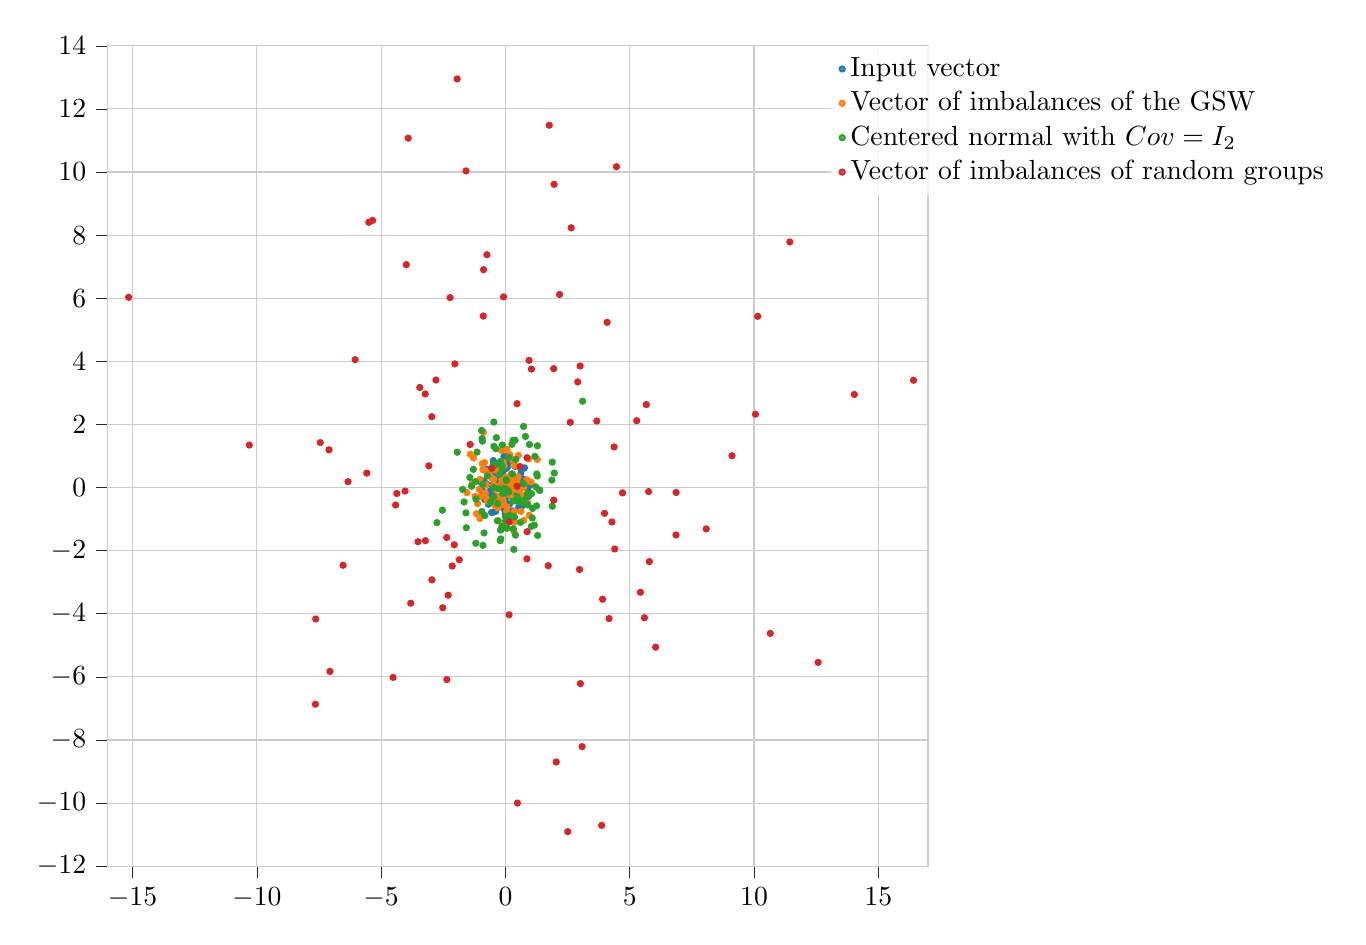
\begin{tikzpicture}

\definecolor{crimson2143940}{RGB}{214,39,40}
\definecolor{darkorange25512714}{RGB}{255,127,14}
\definecolor{darkslategray38}{RGB}{38,38,38}
\definecolor{forestgreen4416044}{RGB}{44,160,44}
\definecolor{lightgray204}{RGB}{204,204,204}
\definecolor{steelblue31119180}{RGB}{31,119,180}

\begin{axis}[
width=12cm,
height=12cm,
axis line style={lightgray204},
legend cell align={left},
legend style={fill opacity=0.8, draw opacity=1, text opacity=1, at={(1.5,1)}, draw=none},
tick align=outside,
tick pos=left,
x grid style={lightgray204},
xmajorgrids,
xmin=-16, xmax=17,
xtick style={color=darkslategray38},
y grid style={lightgray204},
ymajorgrids,
ymin=-12, ymax=14,
ytick style={color=darkslategray38}
]
\addplot [semithick, steelblue31119180, mark=*, mark size=1, mark options={solid}, only marks]
table {%
0.434895013244804 0.124038817819338
-0.171049889611709 -0.318867783508954
-0.655626496516841 -0.18826749725436
-0.0836044232140745 -0.223968334262927
-0.980292787371453 -0.088918833684658
-0.449508209364538 0.461070074401702
-0.578964961919378 0.469199029183644
0.103856769388123 0.765088215409841
-0.870150799568338 0.208479109765157
-0.832925972419536 -0.382088608520988
0.674813576459195 0.597118317057146
0.1406431297911 -0.549597572632135
0.200833409520265 0.939099905288316
-0.103405977636344 -0.347818808453017
-0.212746769279567 0.414798495699087
-0.0022928676872473 0.62972877459891
0.228968759015119 -0.809014684322004
-0.588930256938481 -0.288457500349341
-0.147403197514255 0.329360249896994
-0.803368800971273 -0.282257113184246
0.254162778287603 -0.165993335066653
0.9584167925898 0.0613520103970499
-0.0559610802990755 -0.664516994775544
-0.559427994962747 0.453494206301212
0.0251377309206933 -0.20234264015263
-0.423929908754168 -0.0132535152814863
-0.103583764237094 0.162954447698922
0.824469652102901 0.110380832867433
-0.97416440253291 0.185521552937403
-0.4882834184693 0.853822535632123
0.425419057461674 -0.103915804832133
-0.456287416949303 0.742163129953138
0.151032122408005 0.0916857885384008
-0.0550714362018607 -0.67368595611526
-0.978525643925107 0.172082897004426
-0.7451411443317 0.583097885326367
0.156573573755836 -0.525401378028993
0.889850770051727 -0.300572472296683
0.118353836048231 -0.839052495417782
0.272305725366422 0.859518958544592
-0.0563392612676707 0.982456337784717
0.0910344974245474 -0.663967816196735
0.187925033249884 -0.240153952072305
-0.00781523186832911 -0.827323386846605
-0.0935181499778961 0.146988008326484
0.131675761468232 0.25528152005359
-0.921620521073135 0.108000660214421
-0.398129067082405 -0.758667257268128
-0.478668224780424 -0.25570275761302
-0.556246883923141 -0.788068022594796
-0.322488138211569 0.229978700204299
0.708180964514103 0.268195932674291
0.084351905419851 -0.266426905872132
-0.508490449556374 -0.788213081308513
0.890989027783887 0.140489191907915
-0.0490451897465328 -0.31804567112465
-0.636249904661875 0.37934104338376
-0.21554236054909 0.0579031863312041
0.0263890176690986 -0.564457893477705
-0.369544687834733 0.130040879444561
-0.464990609799235 0.248655556061467
0.941405601701063 -0.27065235631872
-0.112066292056728 0.489010524901944
0.573590259956691 -0.0785610747217894
-0.539915061494033 0.0867533648844998
-0.261490441268277 -0.586790881872528
0.0740915594439333 0.641976082932518
0.895303319522421 -0.0639574486449783
0.0172793229948352 -0.900279013535253
-0.778567805098058 0.123174407041678
0.310434250987342 0.0349470493194343
-0.864211074211286 -0.240466288026837
0.0828019483233264 -0.509562964151696
-0.664657805802782 -0.2068489084593
0.644211651111098 -0.611619050513672
0.0170547507101966 0.598212537250522
0.766988851475884 0.623895151868049
0.773746776384354 0.0642284129694564
-0.658432079253169 -0.502436209565769
-0.363810076049757 -0.325703804242573
-0.350337081489515 0.260539862849042
0.492548817535792 -0.118804075637892
0.300178155249107 -0.740917886129931
-0.614500965616185 -0.104963373605984
-0.24164816052097 -0.487039714932247
-0.526354245938437 -0.333957360249649
0.380817795443004 0.669174608332109
-0.697734320113905 -0.436740535326574
0.326866280596272 -0.0943850298484958
0.615817881215171 0.44221203097473
0.0759728547325323 0.828132687606788
0.0910607835531383 -0.944722254640731
-0.562524161340914 -0.349329717855408
-0.683518680510027 -0.529803975059172
0.594453260858288 0.627504744447079
-0.889149843759688 -0.119617941507995
0.080501646749857 -0.280064098440056
-0.532897234667634 -0.252085236162695
0.0227452842732703 0.986294343042
0.530594052224325 -0.638093548140492
};
\addlegendentry{Input vector}
\addplot [semithick, darkorange25512714, mark=*, mark size=1, mark options={solid}, only marks]
table {%
-0.331088781058578 0.668497913921783
-0.343921836874418 -0.449650239882695
-0.345757214047597 -0.433433458890865
-0.80887175676933 -0.168175802032654
0.456017211681804 0.264872236177079
0.510636987771416 0.34385610295674
-1.11837882636537 -0.511306804185604
-0.333153124617047 -0.274283419438934
0.759650992615713 -0.246506638585994
-1.33854859477777 0.125086429558413
-1.01368441538723 -0.291305575084721
0.256897119250621 0.19013560901107
-1.41495807671361 1.05509689436952
-0.0770504694473546 -0.491366661052502
-0.268258086125591 0.597158453252128
-1.02664091993883 -0.979637597724818
-0.274930326450528 0.0527046477267323
-1.54740235731755 -0.162571992046511
0.534092440317783 -0.286197012822096
-0.726333623356225 -0.430416342671576
-0.839546708797091 0.793981566997718
-0.139844780294531 0.0189660095952668
0.238684944002902 0.438561477407173
-0.148880087703309 -0.2603343095124
-0.932387045876829 0.758274254996264
-0.426507497105139 0.553427172555712
0.751686380642509 0.113724242847771
0.598179212548209 -0.0336284592988055
0.740513058920071 -1.03974293104231
0.572223074528203 0.0255011998215738
-0.102063112378802 -0.324850334980269
0.162699766451511 -0.0257267830711869
0.29106168583092 -0.0504621005454325
-1.284816089712 0.935437821305705
0.938394996774552 0.904893637293057
-0.204460760691326 0.614083046430906
1.28037487560725 0.890633788409664
0.960431270834393 -0.879109947919495
-0.145444371590373 0.238950688195434
0.3011856082923 -0.0653498987210775
0.0539205298233172 0.234129364218935
0.0552511975425656 -0.760314336287323
0.622968599921562 -0.75969995255175
-0.467702735289032 0.0778640718492659
0.422931788281469 -0.0135678523951537
-0.804287425500616 0.532649784049924
-0.390909827860691 -0.0628371366441191
-0.282270794017369 -1.05243251703913
-0.903090829238564 0.565770471981281
0.881097992338106 -0.463581444894688
-0.00461545363010485 0.310800954036489
-0.153001168503635 1.17125131607149
-1.21691045416105 -0.282487708998446
0.156235392667814 0.272955114162047
-0.400697795329167 -0.584914976959752
0.360546934564878 -0.759328312982943
0.0679616164348534 1.20694040633197
-0.0662653640812099 0.0975682582170088
-0.0848867318386893 0.79990495246402
-0.551852365593422 0.298869519442078
-0.309934162377314 -0.646181671539344
-1.02461568787243 0.260412018380637
0.260781335199751 0.321127533169619
0.205601656009753 -0.252138927135721
0.516886677556921 1.0185995568974
1.03090890294832 0.176284352247187
0.0383809420226663 0.326507402384491
-0.0603623956238644 -0.546951271700777
0.215467225188974 0.309015693333237
0.372690586105045 -1.08919615926189
0.315992118531007 0.245560179907878
-0.884836412592866 1.75451193992083
0.353719941320943 0.0142542426354625
-0.0559058368487266 0.689391287738782
0.623840374945824 0.0911412371487048
-0.352041249303223 -0.315300671876331
0.716242748364184 -0.388609638534549
-0.0069648710552539 -0.052309770176735
0.493753979945467 -0.394357342158192
-0.796802755204179 -0.31240660494455
0.528674384933903 -0.119911616009817
-1.05511157203274 -0.0581654463795978
-0.383301308800124 -0.312605657327896
0.30141134416763 0.856522331042485
0.474844113745528 0.265898269567186
0.254817687781489 0.315217073229706
0.859539650565452 0.243319769046367
-0.468792657261908 0.262531606722192
0.138951099716432 -0.146827756829312
0.737975723812107 0.00618269119111636
0.17716318493481 1.04330889002053
0.461490567586713 0.0177916300092141
0.198767966042474 0.12040341840666
0.338651063949415 -1.38375503401006
0.371425716340456 0.692025917075552
-0.648420447958061 0.392225918691415
-1.16161314967886 -0.828971258971103
-0.77321675687382 0.0846801482973339
0.446402517456731 0.322076643375408
0.067510379651106 -0.617750778396911
};
\addlegendentry{Vector of imbalances of the GSW}
\addplot [semithick, forestgreen4416044, mark=*, mark size=1, mark options={solid}, only marks]
table {%
0.729995368005058 1.93580837945654
0.62856598673174 -0.418031055447296
-0.470005611213708 -0.307437178113239
0.0598711439428778 -1.28979873951007
-0.107918461147807 -0.190810775703408
-2.7552443904384 -1.11312494054846
-1.43206380799605 0.320724138473446
0.471731301099324 -0.289578517930905
0.0327794293321657 0.252123597949873
0.474776065539674 -0.438630433467774
-0.945905081856618 -0.758976500539884
-1.66219174010214 -0.458153665921246
-0.486332266769305 0.733722420390866
-0.223412735867732 0.421681593988314
0.038248663900376 0.223071454553962
-0.602555162360409 -0.464406122413479
0.0177674602872895 -0.945139253009986
-1.14239200412958 1.1235871610418
0.0345067545293512 -0.923667776950449
0.263104464394608 1.36969154112307
-1.1820858995249 -0.367426156597115
1.38348296508776 -0.0931314876307586
-1.58843444258787 -0.802161888722233
-0.13402408181269 0.691076551354219
-0.3410112818527 0.730697458444517
0.00462104370858991 -1.0601053518137
-0.380474575408622 1.23098383795141
0.305014829589289 1.49471430373239
-2.53449211813673 -0.716942661950449
0.296955116425069 -0.431464901617827
0.89872008541088 -0.549889621483431
0.174797337670348 -0.885290577460615
1.21849482569737 0.0253040034622034
-1.57292131790976 -1.27529795108113
0.390034585097007 1.4991867572823
-0.92495300008972 1.4686002193045
1.35931237259991 -0.0737433971398373
-1.93614805965176 1.11950007761248
-0.321112065410576 -1.05453942067313
-0.462894163333376 1.30572233305456
-0.125832309838113 1.35001298327061
-0.260080881534807 -0.0377428867519686
1.882326794955 0.80420316354827
-0.828240082732354 -0.886329331152812
0.0981535641843 -0.091174663524401
0.280251899131833 0.428851749714538
-1.21208946708335 0.18695136483169
-0.0270679571304786 -0.0261223491993951
1.26175058240089 0.429922819160211
1.9639664115813 0.458330141669832
-0.467872992790978 0.00499484337820864
-0.133463783071088 -1.22306613670495
0.853868811171843 -0.302940452000001
0.966621651085324 1.36393767075129
-0.958395558822144 1.80696076817015
-0.363236814689279 1.58135965650201
-0.199423888008084 -1.3458016918784
-0.127156511400484 0.583576039497883
1.04397807359125 -1.23108621966842
0.726598190124484 -0.488761285257771
-0.467659128190447 2.07435289741173
-0.914798642686483 0.104357541142446
1.08952876040464 -0.661614419142396
0.40487304365175 -1.50749848191841
1.07809227655561 -0.963954274169064
-0.204786071409268 0.826467909108514
0.339033790016819 -1.96177019063312
-0.209395682669473 -1.68439923963679
0.806310823415416 1.61954291216955
0.899671982794593 -0.17404579678489
-0.168286496279364 -1.32822728766304
1.88609612494423 -0.591169583938084
0.725609765799265 0.119612626994041
-1.3630538664623 0.0412906332107869
1.28072699556658 0.366291005592303
-0.725448590801736 0.36984591739489
-0.936876667843233 1.55347719478912
0.605923975137203 -1.10363425177227
-0.18515492725848 -1.62931864193218
1.29573209877959 -1.52012151482541
0.307023069155429 -0.930481076266289
-0.859670890375738 -1.43836833195895
0.364770651694637 -0.930918472044166
1.1631502554141 -1.1911764333217
-1.19232842401531 -1.76436516030067
-0.311991946320832 -0.511270331458503
-1.28930752515515 0.576006703188704
1.288116730256 1.3251949459554
0.41718005759952 0.888262676834649
0.701910216504962 0.124465117428116
0.12946853065617 0.953637346035052
3.10519019785999 2.73547544315395
-1.71786068013202 -0.0595992243404495
0.317734871740104 -1.30252908414639
-0.902291588086714 -1.83251246039801
1.05187490379466 -0.196441963130579
1.25130193310196 -0.580639888950666
1.18461272094539 0.987451680263202
1.86661996135677 0.235065911041047
0.13651968887717 -0.143457794308217
};
\addlegendentry{Centered normal with $Cov=I_2$}
\addplot [semithick, crimson2143940, mark=*, mark size=1, mark options={solid}, only marks]
table {%
10.1493622389484 5.42636060955185
-0.742499751199785 7.37879948270928
11.4407231457638 7.7839669098855
-5.49429562682395 8.40683800122462
-1.41946832936989 1.36480935830654
-3.44508638826008 3.17234038899514
16.4188545600152 3.40044685245856
-2.35915950939382 -1.58203857463856
-3.91069076783903 11.0726306164627
4.28331682470295 -1.09355721982845
-3.8083932083528 -3.66483599535218
-7.44797389155823 1.42540110675578
2.6077569724878 2.0656236997987
0.4828474458849 -10.0004542907843
9.11375214915861 1.00844223424405
5.78992009601364 -2.34623885146555
4.39607833351426 -1.94735619083139
-3.98676672003448 7.06493902634622
0.154791864008242 -1.09138239538787
3.01679082896783 -6.21388078694246
0.146307560555993 -4.03555552099962
6.86618982101344 -0.156197717317916
4.4660535329762 10.167471642508
-7.09696477560352 1.19476837634445
10.6542273158779 -4.62369087441026
-2.2260123678942 6.01936762057685
3.98793196422703 -0.818033317912658
-3.21820479596866 -1.68383166451406
-7.05957301987748 -5.82933288372992
-0.891792487437045 5.43487163589699
-3.22623181401996 2.9666504901728
1.95913279479532 9.60967394603074
2.64577942700892 8.23190488395692
4.091241714485 5.23667951819513
2.98275381306394 -2.59924738479243
-2.14018692695234 -2.48556488431322
-2.95735275536534 -2.92515951432891
0.585341199543198 0.666592540789878
-10.301255227872 1.34673149851657
2.04326378501673 -8.69872052557584
4.71031000962991 -0.168502741568743
5.28343800245385 2.11899176267022
-4.36895085550197 -0.188737432385034
-1.94194677702017 12.9502233686404
-3.08083135020922 0.687797152431819
-7.64344055134331 -6.8669490644746
0.468169264644391 0.0396088462962497
10.0581770220791 2.32423723649875
-7.63154463827201 -4.16569644715731
-5.57519790704285 0.457451070954488
2.50724201781283 -10.9071069079446
5.43126747417784 -3.32003632844643
-2.30351707684637 -3.41256937120884
2.91011257968499 3.34808670646626
-2.03295731318936 3.91909627225228
-2.35692042010044 -6.0850857839964
-0.0754520305630015 6.04372407104371
1.76423400732163 11.481867578102
3.00569422965304 3.85254128740658
1.9419174832944 3.76745857135422
-4.03664243663295 -0.111890742104821
-0.878931991077556 6.90418508359645
-4.52019977846719 -6.01748958683677
5.66655509787074 2.62975868343347
-1.58423295361029 10.0350436011834
3.87137177564781 -10.7069713934023
4.16796855818616 -4.15315251566002
0.865582506375185 -2.26065945606205
-6.04610672101718 4.05140398705886
5.59129526211391 -4.12649974966477
1.72130580735568 -2.47661137757687
14.0352691770252 2.94915278010849
-3.5167428600955 -1.71680033520227
-4.41647397197922 -0.553760988024869
1.04602503016292 3.75391580072835
3.67557801605528 2.10932077304077
12.5789224155827 -5.54302721806793
0.468363438224959 2.65783475050264
3.08447723875914 -8.21207784948897
2.17750690551774 6.11898562676335
-6.33101219867258 0.185468656670957
-1.85561618006524 -2.28905024960272
3.90851765144073 -3.53940651620429
-0.544192770252372 0.615584399275702
8.07812433206947 -1.31079462603552
1.94288571822675 -0.400302884934945
-15.1557229068269 6.02977976463709
0.951472353457659 4.02933546622984
-2.96065879214263 2.24655797749965
-6.53039255281589 -2.46353728124788
6.86315854363721 -1.50344232546706
0.87222905607385 -1.40017773111298
4.37144565956043 1.28602159802576
-5.3428554943943 8.46701498423381
5.75995081319152 -0.128883374942968
-2.05867314550082 -1.81480951586337
0.869981372959155 0.943679079218688
-2.79620339266121 3.40741982996825
-2.52119461355136 -3.81005353774559
6.04402929937269 -5.060424042555
};
\addlegendentry{Vector of imbalances of random groups}
\end{axis}

\end{tikzpicture}

\caption{Plot of vectors of imbalances of group assignments from the GSW, its input vectors, and samples from a centered normal with $\textbf{Cov}=\textbf{I}_2$ similarly to figure \ref{4types_3}, except we added the vectors of imbalances of random group assignments for comparison. There are 100 input vectors and 100 of each kinds of point, everything is in dimension 2.}
\label{4types_4}
\end{figure}

\begin{figure}
\centering
\newpage
\multido{\i=0+1}{3}{
\includegraphics[width=12.7cm]{3d_example/gswalkboth\i.pdf}
}
\caption{Example of a GSW run with 3 vectors in 2 dimension. The left part shows the cube where the coloring is living, and the right part shows the vector of imbalances and the input vectors.}
\label{3d_example}

\end{figure}


\subsection{Subgaussianity result}\label{results}
%definition for variable, then examples and explain what it means and give alternative conditions and then define for vector
We will first define subgaussianity, which is a way to quantify how centered a random variable or vector is and state a result showing that the vector of imbalances produced by a GSW run is actually $1$-subgaussian.
\begin{definition}\label{def_subgaussianity}
A random variable $X \in \mathbb{R}$ is said to be subgaussian with parameter $\sigma$ (or $\sigma$-subgaussian) if $\forall\lambda\in\mathbb{R}$:
$$\mathbb{E}\left[e^{\lambda(X-\mathbb{E}[X])}\right]\leq e^{\sigma^2\lambda^2/2}$$
\end{definition}
For example, any $\sigma^2$-subgaussian random variable $X$ has $\mathbb{V}[X]\leq\sigma^2$ with equality if it is gaussian. The above definition is equivalent to the following definition based on concentration, which tells us that a centered $\sigma^2$-subgaussian random variable is at least as centered as a gaussian variable with variance $\sigma^2$:
\begin{definition}[Equivalent to definition \ref{def_subgaussianity}]
A random variable $X$ is said to be $\sigma$-subgaussian if $\forall t>0,$ $\max\{\mathbb{P}(X\geq t),\mathbb{P}(X\leq -t)\}\leq exp\left(\frac{-t^2}{2\sigma^2}\right)$.
\end{definition}
This definition is derived from the first one via Chernov's bound. It lets us derive the same kind of useful inequalities about subgaussian random variables as about gaussian variables, which, given that gaussian variables are well-behaved and well-studied, is a desirable feature.

There exists several other equivalent definitions, but the first one is the one-dimensional version of the definition we will use for subgaussianity for random vectors, and the second one helps us understand how subgaussian random variables are related to gaussian variables. 

Now we can adapt the notion of subgaussianity to random vectors:
\begin{definition}[same as definition \ref{def_subgaussianity_intro}]
A random vector $\textbf{Y} \in \mathbb{R}^m$ is said to be subgaussian with parameter $\sigma$ (or $\sigma$-subgaussian) if for all $\bm{\theta} \in \mathbb{R}^m$:
$$\mathbb{E}\left[e^{\langle\textbf{Y},\bm{\theta}\rangle}\right]\leq e^{\sigma^2\|\bm{\theta}\|_2^2/2}.$$
\end{definition}
This definition will help us give a concrete result on the balancing power of the GSW. A random vector being $1$-subaussian means that it is less spread that a gaussian with covariance matrix being the identity. We can see that for the vectors of imbalances of the GSW, on figure \ref{4types_3}, it seems to indeed be the case. This was proved, first for $\sigma^2=40$ in \cite{blues} and then for $\sigma^2=1$ in \cite{harshaw2019balancing}.
\begin{theorem}[\cite{harshaw2019balancing}]
    For $\textbf{z}$ sampled via the Gram-Schmidt walk, we have that $\textbf{Bz}$ is subgaussian with parameter $\sigma^2=1$.%:$$\mathbb{E}[exp(\langle\textbf{Bz},\textbf{v}\rangle)]\leq exp(\|\textbf{v}\|^2_2/2)\quad\forall\textbf{v}\in\mathbb{R}^{n+d}$$
\end{theorem}
This result is necessary to prove that the GSW indeed gives a constructive algorithm for Theorem \ref{banaszczyk}, by using Theorem \ref{equivalence}.

%Result is tight: maybe add something but need to understand well.


%\begin{definition}
%We say that $L\in\mathbb{R}^{n\times n}$ is bounded in the Loewner order by $M\in\mathbb{R}^{n\times n}$, also written as $L\preceq M$ if $M-L$ is positive semi-definite, that is $z^T(M-L)z\geq 0$ $\forall z\in\mathbb{R}^n$.
%\end{definition}
%This other result from \cite{harshaw2019balancing} gives us a bound on the covariance of the vector of imbalances, which tells us that TODO
%\begin{theorem}[\cite{harshaw2019balancing}]
%If all input vectors of the GSW $\textbf{v}_1,\dots,\textbf{v}_n$ have $\ell_2$ norm at most 1, then the covariance
%matrix of the vector of imbalances $Bz$ is bounded in the Loewner order by the orthogonal projection onto the subspace spanned by the columns of $B$: $$Cov(Bz)\preceq P = B(B^TB)^\dagger B^T,$$
%where we recall that $M^\dagger$ is the pseudoinverse of the matrix $M$.
%\end{theorem}
\section{Fast Computations}\label{fast_computations}
Thanks to an original idea from professor Marcus, one can make the GSW run faster than the trivial implementation which takes time $O(n^3d)$ down to $O(n^2d + n^3)$, similarly to what was done in \cite{harshaw2019balancing} using Cholesky factorizations, except the proofs are in our opinion easier to understand. The general idea is similar: at the beginning of a GSW run, we compute some matrices and then during each step of the algorithm, we use only rank one updates to maintain them and derive the update direction from them at each iteration. This results in the removal of an $n$ factor from the asymptotic running time since rank-one update can be computed in quadratic time rather than the cubic time necessary to compute matrix multiplications and inverses.

We first remind the definition of the matrix pseudoinverse:
\begin{definition}
The pseudoinverse $\textbf{M}^\dagger\in\mathbb{R}^{n\times m}$ of a matrix $\textbf{M}\in\mathbb{R}^{m\times n}$ is the unique matrix that verifies:
\begin{enumerate}
\item $\textbf{M}\textbf{M}^\dagger\textbf{M}=\textbf{M}$
\item $\textbf{M}^\dagger\textbf{M}\textbf{M}^\dagger=\textbf{M}^\dagger$
\item $(\textbf{M}\textbf{M}^\dagger)^T=\textbf{M}\textbf{M}^\dagger$
\item $(\textbf{M}^\dagger\textbf{M})^T=\textbf{M}^\dagger\textbf{M}$
\end{enumerate}
\end{definition}
The pseudoinverse is basically a generalization of the inverse for singular and non-square matrices. In particular $\textbf{P}=\textbf{M}\textbf{M}^\dagger$ is the orthogonal projector onto the column space of $\textbf{M}$.

For some set $S\subset\{1,\dots,n\}$, let $\textbf{I}_S\in\mathbb{R}^{n\times n}$ be the diagonal $n\times n$ matrix with $\textbf{I}_S(i,i) =1$ if $i\in S$ and $0$ otherwise, and $\textbf{B}_S\in\mathbb{R}^{d\times n}$ be $\textbf{BI}_S$ where $\textbf{B}$ is as previously the matrix containing the input vectors as columns. We define $\textbf{C}_S\in\mathbb{R}^{n\times d}$ to be such that $\textbf{C}_S\textbf{B}_S=\textbf{I}_S$ and if $i\not\in S$, the $i$th row of $\textbf{C}_S$ is $\textbf{0}$. That is, the rows of $\textbf{C}_S$ whose index are in $S$ are the pseudo-inverse of the corresponding columns in $\textbf{B}_S$. Finally, $\textbf{D}_S\in\mathbb{R}^{n\times n}$ is $\textbf{C}_S\textbf{C}_S^T$.

This technique necessitates that the dimension of the space spanned by the input vectors is at most the dimension $d$ of the input vectors, as otherwise $\textbf{C}_S$ doesn't exist. One way to adapt it to the other cases is to add an identity matrix multiplied by some small factor at the bottom of the $\textbf{B}_S$ matrix. That way, we can reduce it to the case where the space spanned by the vectors is large enough, and the results differ only very slightly from those we'd obtain via conventional computational methods. This technique does introduce some numerical issues for big $n$ and $d$ though, and it seems preferable to use a more conventional implementation of the GSW in this case. Another way would be to use a parameter and basically apply the GSW design from\cite{harshaw2019balancing} with a very small $\phi$, which would be similar to the previous technique outside of the scale.

Here are the rank one updates that let us compute our matrices for some $S'=S\setminus\{k\}$.
\begin{lemma}\label{update_lemma}
For $k\in S$, let 
\begin{itemize}
\item $\textbf{c}_k\in\mathbb{R}^{n}$ be the $k$th row of $\textbf{C}_S$
\item $\textbf{d}_k\in\mathbb{R}^{d}$ be the $k$th row of $\textbf{D}_S$
\item $S'= S\setminus\{k\}$
\end{itemize}
Then $\textbf{C}_{S'}=\textbf{C}_S-\frac{1}{\textbf{d}_k(k)}\textbf{d}_k\textbf{c}_k^T$ and $\textbf{D}_{S'}=\textbf{D}_S-\frac{1}{\textbf{d}_k(k)}\textbf{d}_k\textbf{d}_k^T$.
\end{lemma}
\begin{proof}
For the first part, we have that\begin{align*}
\left(\textbf{C}_S-\frac{1}{\textbf{d}_k(k)}\textbf{d}_k\textbf{c}_k^T\right)\textbf{B}_{S'}&=\left(\textbf{C}_S-\frac{1}{\textbf{d}_k(k)}\textbf{d}_k\textbf{c}_k^T\right)\textbf{B}_{S}\textbf{I}_{S'}\\
&=\textbf{C}_S\textbf{B}_S\textbf{I}_{S'}-\frac{1}{\textbf{d}_k(k)}\textbf{d}_k\textbf{c}_k^T\textbf{B}_{S}\textbf{I}_{S'}\\
&=\textbf{I}_{S'}-\frac{1}{\textbf{d}_k(k)}\textbf{d}_k\textbf{e}_k^T\textbf{I}_{S'}\\
&=\textbf{I}_{S'}-\frac{1}{\textbf{d}_k(k)}\textbf{d}_k\textbf{0}\\
&=\textbf{I}_{S'}\end{align*}
Thus we just need to show that the rows of $\textbf{C}_S-\frac{1}{\textbf{d}_k(k)}\textbf{d}_k\textbf{c}_k^T$ not in $S'$ are \textbf{0}. As $\frac{1}{\textbf{d}_k(k)}\textbf{d}_k(k)=1$, we have that the $k$th row of $\textbf{C}_S-\frac{1}{\textbf{d}_k(k)}\textbf{d}_k\textbf{c}_k^T$ is indeed \textbf{0}. Lastly, as $\textbf{D}_S=\textbf{C}_S\textbf{C}_S^T$, we have that $i\not\in S\Rightarrow \textbf{d}_k(i)=0$ thus all the rows whose indices aren't in $S$ indeed do stay \textbf{0}.

For the second part, we can see that \begin{align*}
\textbf{D}_{S'}&=\textbf{C}_{S'}\textbf{C}_{S'}^T\\
&=\left(\textbf{C}_S-\frac{1}{\textbf{d}_k(k)}\textbf{d}_k\textbf{c}_k^T\right)\left(\textbf{C}_S-\frac{1}{\textbf{d}_k(k)}\textbf{d}_k\textbf{c}_k^T\right)^T\\
&=\left(\textbf{C}_S-\frac{1}{\textbf{d}_k(k)}\textbf{d}_k\textbf{c}_k^T\right)\left(\textbf{C}_S^T-\frac{1}{\textbf{d}_k(k)}\textbf{c}_k\textbf{d}_k^T\right)\\
&=\textbf{C}_S\textbf{C}_S^T-\frac{1}{\textbf{d}_k(k)}\textbf{C}_S\textbf{c}_k\textbf{d}_k^T-\frac{1}{\textbf{d}_k(k)}\textbf{d}_k\textbf{c}_k^T\textbf{C}_S^T+\frac{1}{\textbf{d}_k(k)^2}\textbf{d}_k\textbf{c}_k^T\textbf{c}_k\textbf{d}_k^T\\
&=\textbf{D}_S-\frac{1}{\textbf{d}_k(k)}\textbf{d}_k\textbf{d}_k^T-\frac{1}{\textbf{d}_k(k)}\textbf{d}_k\textbf{d}_k^T+\frac{1}{\textbf{d}_k(k)}\textbf{d}_k\textbf{d}_k^T\\
&=\textbf{D}_S-\frac{1}{\textbf{d}_k(k)}\textbf{d}_k\textbf{d}_k^T\end{align*}\end{proof}
Now let's see why this is useful, that is, how to compute $\textbf{v}^\perp(t)$ and $\textbf{u}_t$ from these matrices.
\begin{lemma}
Assume we're currently in a step of the GSW where the active vectors are $A_t=\{\textbf{v}_s:s\in S\}$, and $\textbf{v}_k\in A_t$ is the pivot. If $\textbf{d}_k$ and $\textbf{c}_k$ are defined similarly as in Lemma \ref{update_lemma}, we have that $$\textbf{v}^\perp(t)=\frac{\textbf{c}_k}{\|\textbf{c}_k\|^2}\textrm{ and }\textbf{u}_t=\frac{\textbf{d}_k}{\textbf{d}_k(k)}.$$
\end{lemma}
\begin{proof}
Let $S'=S\setminus \{k\}$. Starting from the definition of $\textbf{v}^\perp(t)$ with pivot $p(t)=k$, we have that \begin{equation*}\begin{WithArrows}
\textbf{v}^\perp(t)&=\Pi_{V_t^\perp}(\textbf{v}_k)\Arrow{$\Span V_t\cup V_t^\perp=\mathbb{R}^d$}\\
&=\textbf{v}_k-\Pi_{V_t}(\textbf{v}_k)\Arrow{Definition of $\Pi_{V_t}$ with pivot $k$}\\
&=\textbf{v}_k-\textbf{B}_{S'}\textbf{C}_{S'}\textbf{v}_k\Arrow{Lemma \ref{update_lemma}}\\
&=\textbf{v}_k-\textbf{B}_{S'}\left(\textbf{C}_S-\frac{1}{\textbf{d}_k(k)}\textbf{d}_k\textbf{c}_k^T\right)\textbf{v}_k\Arrow{$\textbf{C}_i\textbf{v}_k^T=\mathds{1}_{i=k}$}\\
&=\textbf{v}_k-\textbf{B}_{S'}\textbf{e}_k+\frac{1}{\textbf{d}_k(k)}\textbf{B}_{S'}\textbf{d}_k\textbf{c}_k^T\textbf{v}_k\Arrow{$k$th line of $\textbf{B}_{S'}$ is \textbf{0} as $k\not\in S'$}\\
&=\textbf{v}_k+\textbf{0}+\frac{1}{\textbf{d}_k(k)}\textbf{B}_{S'}\textbf{d}_k\Arrow{$\textbf{d}_k$ is the $k$th row of $\textbf{D}_S=\textbf{C}_S\textbf{C}_S^T$}\\
&=\textbf{v}_k+\frac{1}{\textbf{d}_k(k)}\textbf{B}_{S'}(\textbf{e}_k^T\textbf{C}_S\textbf{C}_S^T)^T\Arrow{$(\textbf{AB})^T=\textbf{B}^T\textbf{A}^T$}\\
&=\textbf{v}_k+\frac{1}{\textbf{d}_k(k)}\textbf{B}_{S'}\textbf{C}_S\textbf{C}_S^T\textbf{e}_k\\
&=\textbf{v}_k+\frac{1}{\textbf{d}_k(k)}\textbf{B}_{S'}\textbf{C}_S\textbf{c}_k\Arrow{Definition of $\textbf{B}_{S'}$} \\
&=\textbf{v}_k+\frac{1}{\textbf{d}_k(k)}\left(\textbf{B}_{S}-\textbf{v}_k\textbf{e}_k^T\right)\textbf{C}_S\textbf{c}_k\\
&=\textbf{v}_k+\frac{1}{\textbf{d}_k(k)}\textbf{B}_{S}\textbf{C}_S\textbf{c}_k^T-\frac{1}{\textbf{d}_k(k)}\textbf{v}_k\textbf{c}_k^T\textbf{c}_k\Arrow{$\textbf{D}_S=\textbf{C}_S\textbf{C}_S^T$}\\
&=\textbf{v}_k+\frac{1}{\textbf{d}_k(k)}\textbf{B}_{S}\textbf{C}_S\textbf{c}_k^T-\frac{\textbf{d}_k(k)}{\textbf{d}_k(k)}\textbf{v}_k\\
&=\frac{1}{\textbf{d}_k(k)}\textbf{B}_{S}\textbf{C}_S\textbf{c}_k^T\Arrow{Pseudo-inverse definition}\\
&=\frac{1}{\textbf{d}_k(k)}(\textbf{B}_{S}\textbf{C}_S)^T\textbf{c}_k^T\Arrow{$(AB)^T=B^TA^T$}\\
&=\frac{1}{\textbf{d}_k(k)}\textbf{C}_S^T\textbf{B}_{S}^T\textbf{c}_k^T\Arrow{Pseudo-inverse definition}\\
&=\frac{1}{\textbf{d}_k(k)}\textbf{c}_k^T\Arrow{$\textbf{D}_S=\textbf{C}_S\textbf{C}_S^T$}\\
&=\frac{1}{\|\textbf{c}_k\|^2}\textbf{c}_k^T
\end{WithArrows}\end{equation*}

For the second part, we have that $\textbf{u}_t$ is the solution to the system \begin{align*}\textbf{u}_t(k) =1\\
            \textbf{u}_t(i) =0 \text{ if } i \notin A_t\\
            \textbf{v}^\perp(t) = \textbf{v}_{k} + \sum_{i \in A_t\setminus\{p(t)\}} \textbf{u}_t(i)\textbf{v}_i=\textbf{B}_S\textbf{u}_t\end{align*}
But we have that $$\textbf{v}^\perp(t)=\frac{\textbf{c}_k}{\|\textbf{c}_k\|^2}=\frac{\textbf{C}_S^T\textbf{e}_k}{\|\textbf{c}_k\|^2}$$
if we multiply by $\textbf{C}_S$ we get $\frac{\textbf{C}_S\textbf{C}_S^T\textbf{e}_k}{\|\textbf{c}_k\|^2}=\textbf{u}_t$ But as $\textbf{C}_S\textbf{C}_S^t=\textbf{D}_S$ and $\|\textbf{c}_k\|^2=\langle \textbf{c}_k,\textbf{c}_k\rangle=\textbf{d}_k(k)$, we have that indeed $\frac{\textbf{d}_k}{\textbf{d}_k(k)}=\textbf{u}_t$.
\end{proof}
These lemmas mean that once we have computed $\textbf{C}_S$ and $\textbf{D}_S$ at the beginning of the GSW in time $O(n^2d+n^3)$, we update them at most $n$ times in $O(nd+n^2)$ operations and store them with a similar quantity of memory, resulting in a total time of running of $O(n^2(d+n))$ as computing $\delta_t$ and updating the coloring takes $O(n)$ time.

This happens to not be much faster in practice than a clever implementation using rank-one update to compute the inverse necessary to compute the least squares solution. That is because in the latter case, the size of the inverse matrix decreases at each step of the algorithm in that case, thus the one matrix multiplication necessary to compute the update direction becomes faster than the rank one updates described in this section quickly when $n$ is small, as $\textbf{C}_S$ and $\textbf{D}_S$ keep the same size throughout the whole algorithm run.


\section{Generalizing to any Hyperparallelepiped}\label{different_basis_section}
The idea is to allow the algorithm to produce colorings not only on the hypercube $[-1,1]^n$, but also on any hyperparallelepiped spanned by a set $\textbf{b}_1,\dots, \textbf{b}_n\in\mathbb{R}^n$ of $n$ linearly independent vectors, denoted as the basis $\mathcal{B}$. The assignment returned then won't be a coloring per se but just a linear combination of the vectors with some coefficients corresponding to a vertex of the hyperparallelepiped formed by the basis vectors that should hopefully yield a somewhat short vector of imbalances. We will still denote it by the term coloring for clarity reasons.

To do so, we have to adapt the algorithm at several points. Firstly, an element $k$ associated to the basis vector $\textbf{b}_k$ should be alive only if the current coloring is not on one of the 2 facets such that when expressed in the basis $\mathcal{B}$, the $k$th coordinate is -1 or 1. 

Secondly, choosing the update direction is then different as we need to stay orthogonal from every fixed vector, but these vectors do not correspond to coordinates anymore as we're not using the trivial basis $\textbf{e}_1,\dots,\textbf{e}_n$ anymore.

Thirdly, the computation of the two potential $\delta$ is different as well for some similar reasons: you have to compute the maximum delta such that the coloring stays in the hyperparallelepiped defined by the basis.

All these issues can be solved via some basis changes in the right spots and the modified algorithm is very similar, and should work exactly the same way when given the orthonormal canonical basis of $\mathbb{R}^n$, $\textbf{e}_1,\dots,\textbf{e}_n$. The main idea is that we will keep two separate coloring, $\textbf{z}$ and $\textbf{z}'$, where $\textbf{z}$ is expressed in the canonical basis and $\textbf{z}'$ is expressed as coordinates in $\mathcal{B}$. We will update $\textbf{z}'$ with $\textbf{u}_t'$, that is $\textbf{u}_t$ except it is expressed via its coordinates in $\mathcal{B}$. Computing $\delta_t$ is then fairly easy as we just have to replace $\textbf{z}$ by $\textbf{z}'$ in the normal computation. 

Let $\textbf{B}_{\mathcal{B}}$ be the matrix containing the basis vectors $\textbf{b}_1,\dots,\textbf{b}_n$ as columns. In order to compute $\textbf{u}_t'$, we replace the matrix containing our input vectors as columns, $\textbf{B}$, by $\textbf{B}\textbf{B}_{\mathcal{B}}$. We then apply the same method as usual to find $\textbf{u}_t'$, and change its basis to get $\textbf{u}_t$.

Putting it all in pseudocode and highlighting the difference with the original algorithm (\ref{walk}) in \textcolor{red}{red}, we get the Algorithm \ref{basiswalk}.\\
\begin{algorithm}[H]\label{basiswalk}
{\fontsize{10}{12}
\caption{The Gram-Schmidt walk on a different basis}
    \SetKwInOut{Input}{Input}
    \SetKwInOut{Output}{Output}
    \Input{$\textbf{v}_1,\ldots,\textbf{v}_n\in\mathbb{R}^d$%with $\ell_2$ norm  at most 1
, an initial coloring $\textbf{z}_0\in[-1,1]^n$,   \textcolor{red}{$n$ linearly independent basis vectors $\textbf{b}_1,\dots,\textbf{b}_n\in\mathbb{R}^n$}}
    \Output{a coloring $\textbf{z}_n \in \textcolor{red}{\mathbb{R}^n}$}
   \textcolor{red}{$\textbf{z}_0'=\textbf{B}_{\mathcal{B}}^{-1}\textbf{z}_0$}\\
   $A_1=\{i\in[n]:|\textbf{z}_0'(i)|<1\}$, $n(1) = \max \{i \in A_1\}$ and $t=1$.\\
    \textcolor{red}{$\textbf{B}=(\textbf{v}_1,\dots,\textbf{v}_n)\textbf{B}_{\mathcal{B}}$}\\
    \While{$A_t\not=\emptyset$}{
        Compute $\textcolor{red}{\textbf{u}_t'}\in\mathbb{R}^n$ such that
        $\begin{cases}
              \textcolor{red}{\textbf{u}_t'}(p(t)) =1\\
              \textcolor{red}{\textbf{u}_t'}(i) =0 \text{ if } i \notin A_t\\
            \textbf{v}^\perp(t) =   \textcolor{red}{\textbf{B}\textbf{u}_t'}\\
        \end{cases}$\\
        $\Delta = \{\delta : \textcolor{red}{\textbf{z}_{t-1}' + \delta \textbf{u}_t'} \in [-1,1]^n\}$, let $\begin{cases}
            \delta_t^+ = \max \Delta\\
            \delta_t^- = \min \Delta
        \end{cases}$
         then $\delta_t = \begin{cases}
            \delta_t^+ \text{ w.p. } \frac{-\delta_t^-}{(\delta_t^+ - \delta_t^-)}\\
            \delta_t^- \text{ w.p. } \frac{\delta_t^+}{(\delta_t^+ - \delta_t^-)}
        \end{cases}$\\
        $  \textcolor{red}{\textbf{z}_t' = \textbf{z}_{t-1}' + \delta_t \textbf{u}_t'}$, $t\leftarrow t+1$,  $A_t=\{i\in[n]:|  \textcolor{red}{\textbf{z}_{t-1}'}(i)|<1\}$, $p(t) = \max \{i \in A_t\}$.
    }
    Output $  \textcolor{red}{\textbf{B}_{\mathcal{B}}\textbf{z}_t'\in\mathbb{R}^n}$.
    %\caption{Gram-Schmidt walk}
    }%
    \end{algorithm}
An example of output of the GSW with a different coloring basis can be found in figure \ref{3types_basis_200_2}, that contains a plot of vectors of imbalances of the classical GSW, and the GSW with two different basis; one that is all positive vectors of norm 1 and one that is orthonormal. We see that the vectors of imbalances of the latter resemble closely those of the classical GSW, while those obtained using the former have a skewed distribution. 
\begin{figure}[h!]
% This file was created with tikzplotlib v0.10.1.
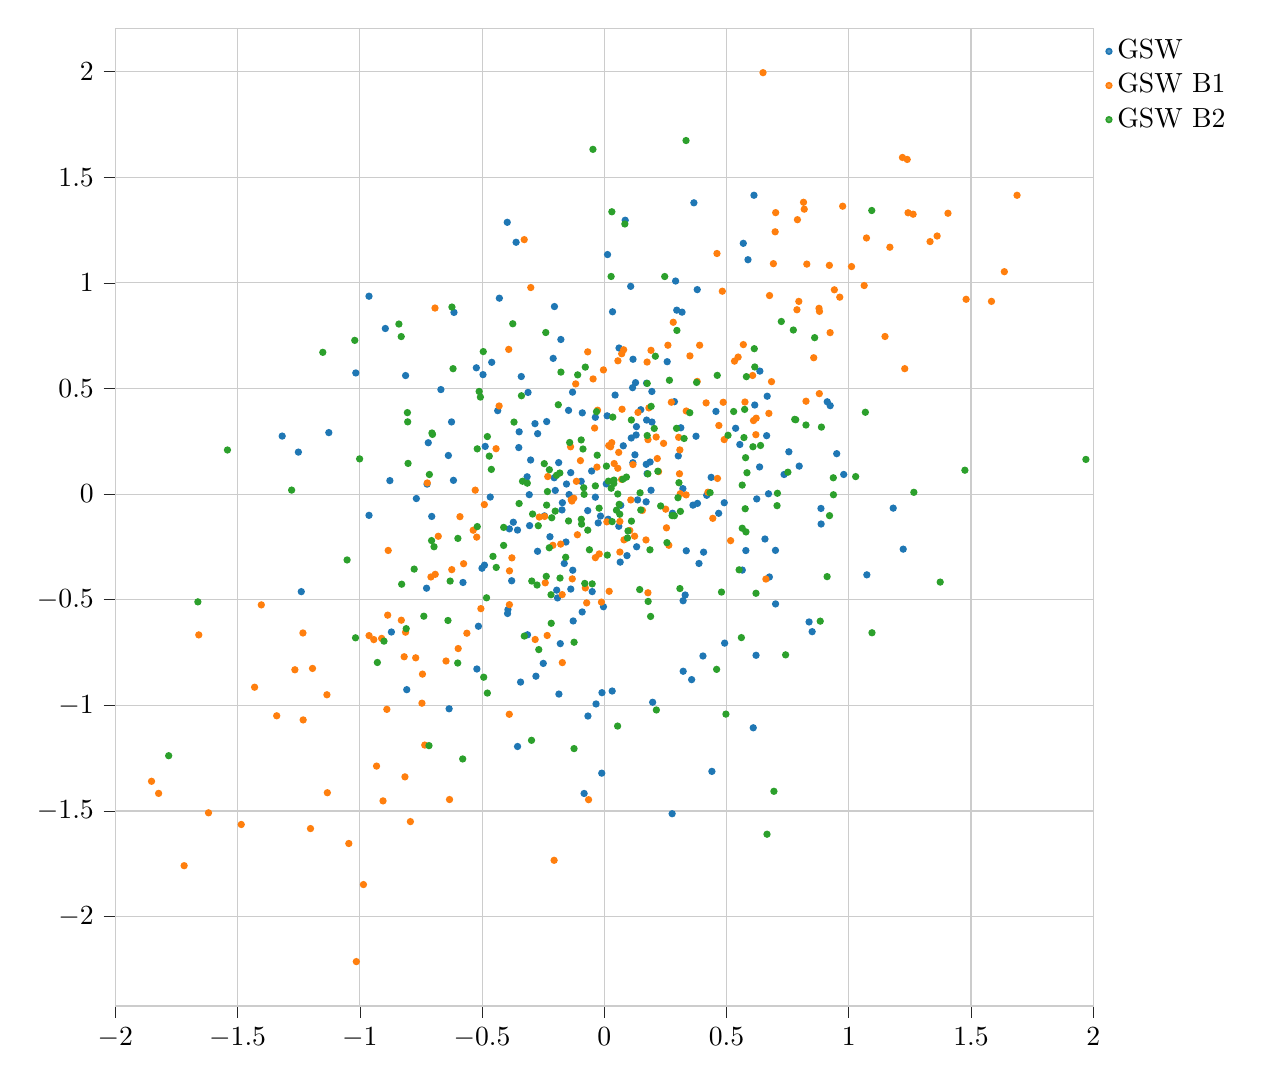
\begin{tikzpicture}

\definecolor{darkorange25512714}{RGB}{255,127,14}
\definecolor{darkslategray38}{RGB}{38,38,38}
\definecolor{forestgreen4416044}{RGB}{44,160,44}
\definecolor{lightgray204}{RGB}{204,204,204}
\definecolor{steelblue31119180}{RGB}{31,119,180}

\begin{axis}[
width=14cm,
height=14cm,
axis line style={lightgray204},
legend cell align={left},
legend style={fill opacity=0.8, draw opacity=1, text opacity=1, at={(1.15,1)}, draw=none},
tick align=outside,
tick pos=left,
x grid style={lightgray204},
xmajorgrids,
xmin=-2, xmax=2,
xtick style={color=darkslategray38},
y grid style={lightgray204},
ymajorgrids,
ymin=-2.42351342052222, ymax=2.20522790588305,
ytick style={color=darkslategray38}
]
\addplot [semithick, steelblue31119180, mark=*, mark size=1, mark options={solid}, only marks]
table {%
-0.272989397532642 -0.270830168705098
0.700187481736672 -0.26644850286336
-0.768711787604231 -0.0211970775021204
-0.514816886189661 -0.625651480096859
-0.235608473294304 0.343147318784805
-0.339556699734259 0.556443744286873
-1.25131223576658 0.19865589630816
-0.094500876597668 0.0604039927086589
-0.156844719755616 -0.226988755656964
-0.185610062198773 -0.946759789671061
0.27899659698643 -0.0906639181599249
-0.43598928373945 0.394864355195059
0.085524989452342 1.29619946185861
-0.70585404481079 -0.105831448526834
0.127905864180179 0.52736754175941
-0.578064726154913 -0.418463587226206
0.636371616255323 0.582037254661137
0.366507433995956 1.37875308035821
0.440190504567662 -1.31271459218328
0.175205715454053 0.0967759292853775
-0.0516471779529777 0.108980741395135
-0.0677588610137263 -0.078248662565601
-0.24961029763121 -0.801551070035558
0.187354773684068 0.151761961864789
0.357344805931162 -0.878405363530902
0.467919897160944 -0.091069213619337
-0.668391151445344 0.494674762111966
0.291733635066145 1.00848039658018
0.924062037480881 0.418517478803971
0.490729062132094 -0.0409119669705438
0.0117382041469121 0.370412971171631
-0.144014861864114 -0.00229711791597431
-0.127300403072011 -0.600624066352283
0.609406620175927 -1.10635452620402
0.0675231780067286 -0.0535129821638548
-0.128941630103358 -0.360447745600827
0.666401947197687 0.463215319916414
-1.12681358215024 0.290935132626698
0.130161778177891 0.279783269086956
0.587794906564519 1.10943412380808
0.43728236545714 0.0791329967115055
-0.137045702636277 -0.449716739162477
-0.490149147442417 -0.336468344036519
0.32274898992102 -0.838794861205872
0.40360689063602 -0.766418568203415
0.125303426764774 0.185909623829649
-0.137229180894652 0.10143869851915
0.635284435566051 0.128378291962097
-0.877097439589344 0.0637480473303991
-0.0103929510348522 -1.32114715507385
0.116953842550714 0.148353095966962
-1.01650840474521 0.573374067706374
0.257380403075728 0.626640455957408
-0.200496563999681 0.0171940849784445
0.9793944568121 0.0928003355759227
-0.179996442838915 -0.707950860442317
-0.186514812322545 0.148890252554748
-0.429190272547465 0.927265746575673
0.0650359361308956 -0.322112676036525
-0.37208267491134 -0.133302782844747
0.194663304516295 0.485697516759429
0.886327139060989 -0.0679729190433543
-0.388280167182582 -0.16461692889131
0.375197824315727 0.273776001285907
0.0593309517052665 -0.152521470499451
0.0158384347802101 -0.11916213346202
-0.0904954014889349 -0.557917969657021
0.418878916226088 -0.00591570070160197
-0.313967331878069 -0.66612453270273
0.0132770420769186 1.13375499421042
0.277577112286873 -1.51305623788977
0.579102533760345 -0.26734319063814
0.0081092363170796 0.0482315867524721
0.387399722101993 -0.328429801132599
0.13621963132662 -0.0274788533923024
0.32150897467824 0.0256674459569664
0.313078061187394 0.313869728716891
-0.0899461195030762 0.384559413268573
0.664120246133247 0.276455663101841
-0.163692629189088 -0.328584993585425
-0.487184189835157 0.225637477639962
-0.348208137042324 0.294819474585352
-0.360744713627773 1.19201144739004
-0.355025383227382 -0.17036415562812
-0.0336663573936742 -0.993478927469238
-0.637782926301786 0.182645074800465
0.615495599593746 0.421492459797501
0.115728621055569 0.503641818063717
-0.129834586804201 0.482492294894594
-0.191270007413167 -0.491562847429276
-0.154672117587084 0.0475309114650236
0.318077886996915 0.861118147128681
-0.727006223899297 -0.445545853351879
0.171638212845094 0.140815865011391
-0.349773650244402 0.220094740383598
0.950769644457184 0.191233064543686
-0.272590899513208 0.2859408957318
-0.315662692188764 0.0818760047648059
1.22279359878879 -0.260720612765816
-0.0824572595394142 -1.41727499139437
-0.724894178903151 0.0472379875780725
0.322443426782933 -0.504931664927734
0.0928737530394599 -0.29133172229245
-0.0364793448089635 -0.0145884807096253
0.197819842318758 -0.985543262975574
-0.466488383913576 -0.0141219642516305
-0.617061622548195 0.06503386135921
0.850316881850824 -0.651303985955301
-0.203901033254816 0.88765646505629
-0.81276105596091 0.561063116022576
0.132307595664567 -0.249421958304766
0.837723573550919 -0.60526946581883
0.173177690434373 0.350253922118752
0.797305394212733 0.132307061920515
0.537285964855374 0.311500417981963
-0.209051383054709 0.642356982297813
0.45667172552766 0.391293731880115
-0.624795379185715 0.341554559265708
-1.31763483476802 0.274508849691271
-0.244844456849802 -0.103149583201972
0.735537936546285 0.0926948718842941
-0.460475849538881 0.623731299323192
-0.500290809104046 -0.351022339403719
0.657218130468473 -0.21271341135747
0.0442606325349251 0.468624164089932
-0.311864045412977 0.481198208796759
-0.962460070164498 -0.100654081892429
0.330849083918251 -0.477778209001128
1.1818696555467 -0.0666028379920198
0.675352423009156 -0.392535535129945
0.554427267148322 0.23467571096736
0.110370815972285 0.265527135421264
-0.0668971509884764 -1.05069354511142
0.0603682158845757 0.691418766594005
1.07404697272909 -0.382351092812964
-0.146178571522589 0.39623313731996
-0.395618878415454 -0.565216042878378
-1.23951947586476 -0.461855992954947
-0.521189435130551 -0.828018882069905
-0.305513166490366 -0.149349956475667
0.077692283303521 0.228486128876235
0.620804343252234 -0.763164360020054
0.564595975550175 -0.359807256515341
-0.396890851537821 1.28647480168682
-0.00346542959059781 -0.533339547909543
-0.0365649778555646 0.363547999476739
-0.306890524085884 -0.00278051130225421
-0.962487928899534 0.936633895742968
0.195025916469944 0.340942535327711
-0.177658661769414 0.731740301337297
0.0337768005571206 0.862941490436239
0.131554533952202 0.319156836205479
-0.614867433867863 0.860027723629613
0.296441371202404 0.870531827786039
-0.378850720642021 -0.410432366622615
-0.634693636989585 -1.01629068927488
-0.342440277687589 -0.890043211344307
0.149245851569494 0.399381590993062
-0.204920131038438 0.0772252613512489
0.171176263394029 -0.0367996901991798
-0.354795453404829 -1.19485386729482
-0.87081398726507 -0.652988435898114
-0.0494538408347232 -0.461631088237309
-0.394176172753152 -0.547157496395115
0.107928104190106 0.983333897444079
0.492302734312742 -0.705621882660152
0.406174897256145 -0.274950616890545
0.381107090684857 -0.0441153421957075
-0.0248962913620925 -0.136448047862363
-0.895698924019663 0.78382173642651
0.755011293924191 0.200165025149238
0.612274836094199 1.41448713941871
0.380222792648295 0.967849997615986
0.362712259291352 -0.0523964360025804
-0.279660580351303 -0.862185165039541
0.191292230201972 0.0180768361899827
-0.00945032246046651 -0.940152800202903
-0.283524122625028 0.333338651174106
-0.0154282517436217 -0.104175355870214
0.700652595240422 -0.519998438099215
-0.72007142031317 0.243040549439289
-0.496086533419957 0.565433793592822
0.302747221323641 0.180647681672578
-0.171410067755586 -0.0408763611474798
-0.301358060554892 0.16125833070622
0.911970896144654 0.436807066123755
-0.222302054645712 -0.201919264361081
0.117582930090358 0.638149708244905
0.568606447225747 1.18696081968955
0.67172853819528 0.00129492478479232
-0.5233198557833 0.597721695562112
-0.173038843501017 -0.075004736027783
-0.808058720030928 -0.925852616323411
-0.194645980419492 -0.454814609932209
0.623575300262468 -0.0229711097052517
0.335407751603929 -0.268386267930265
0.286845360351033 0.437491509320642
0.032309975840203 -0.932283731702294
0.886931644519491 -0.141705737504366
0.173074274882009 0.524954649639963
};
\addlegendentry{GSW}
\addplot [semithick, darkorange25512714, mark=*, mark size=1, mark options={solid}, only marks]
table {%
-1.13463640373959 -0.95001587331791
-0.172312293920437 -0.475921905923077
0.0712502540564861 0.664238072916169
0.460919132391949 1.13883139984953
1.26337374552266 1.32468247994671
-0.0720114132023468 -0.515049634611152
-0.244001696600204 -0.105712314419312
0.701048782592441 1.33223850381757
0.212252037382104 0.27010803219149
-0.116990372875095 0.521529326137612
0.251232561601422 -0.0715048080620437
0.817956724474108 1.34859901404662
0.490552742302911 0.257907917534215
-0.0678026452161311 0.673249047301735
-0.623861471730925 -0.35771023941722
0.117332157978622 0.139730346361546
1.68851877634563 1.41439034074327
-0.0364991770790476 -0.301024048945347
-1.2318066918348 -1.06908431948219
-0.390917766506611 0.684817001669532
-0.0299844918799868 0.127640242548071
0.191093676775282 0.680450726450331
0.443846668700966 -0.114906491548952
0.920701018237739 1.08271660427696
0.482808662026196 0.960263442028592
-0.830239598285107 -0.597085333633902
-1.23276703389132 -0.657482901061376
-0.097558709297152 0.158366505389518
-0.590438158331568 -0.10689007384925
-1.85210472366785 -1.35961634849358
0.335246389792605 0.393177109035479
0.254330540965522 -0.159832138257939
-0.691566457078866 -0.379934172775712
0.175099803589281 0.624909276359494
0.182462644756575 0.407883314262039
1.33265842746604 1.19521750118127
0.178480555318947 -0.467126698685596
-0.94296092209891 -0.688848965525652
-1.20182741344299 -1.58341054534629
-1.04505458238679 -1.6540232790316
-0.883869169049278 -0.266837293003851
-0.124846593742357 -0.0195573361906539
-1.43046791715928 -0.914245307432744
0.790063759871856 1.298781366018
-1.19351629847836 -0.825368076300709
1.23916482727961 1.58407750210534
-0.0642995517647121 -1.44663756217977
0.6200296475789 0.281194478707883
-0.504813455302034 -0.542286487197729
0.547462004931672 0.648602481515209
0.104478327642513 -0.172138003237775
0.698986051423119 1.24146120393727
1.0725256867622 1.21226038032364
0.334784851622763 -0.00376733464952242
0.307600247701036 0.0960885711323393
1.58382946117533 0.912269565879583
-0.562139304423206 -0.658726157480722
0.795771510786494 0.912066865406662
0.941149833300363 0.966946318407591
0.0199811496456734 -0.46030835059078
-1.0142680585706 -2.21311608750379
0.923797997780981 0.764210318718092
0.137844103877812 0.386557131892663
-1.71862570254299 -1.75909446460791
0.610443492211676 0.347912547458277
-0.818554044423029 -0.77003718990372
1.63649276114086 1.05270024967653
1.14830287163185 0.745936622724882
-0.077495492924248 -0.444286500503341
1.40592242368929 1.32931050965137
-0.709156248060519 -0.392320737623976
-0.132435426467962 -0.0329759558883478
-0.327484205038508 1.2044647115677
0.26022206947384 0.704656990890023
-0.793184252484672 -1.5504268003792
0.568833256616371 0.70757853101533
-0.597588738776807 -0.731291603886266
0.0305088854704973 0.243251168307392
-0.114059400908748 0.0603941220673613
0.828523752317229 1.08855315079229
0.60676874451474 0.561490498882454
-0.210398659635728 -0.242670334984789
-0.931546192960596 -1.28763577125835
0.063802893131582 -0.274443205679809
-0.812926361773572 -0.653859202668117
0.675956406918293 0.939792831812196
0.310816927185128 0.00171388764513689
1.06312235562488 0.987188298230865
0.825192188865678 0.439622868930248
0.018176785340157 0.229532701737793
-0.575535962352448 -0.329673457544223
0.178785180984378 0.257732262644352
1.01138050412282 1.07695460545964
0.673240752967536 0.381939855094265
-1.82306765507121 -1.41677731552552
0.649321444150518 1.99483057286463
0.516828605176769 -0.220471932181302
-0.679156138176844 -0.199749993351222
-1.13286470122255 -1.41373258738459
-0.377974949433404 -0.301917129663456
0.0557056870749482 0.630755797411948
0.814949105574401 1.38132642022315
1.22906148088044 0.593652272451647
-0.265907637937287 -0.108844491984424
0.788099074795696 0.872487315713509
1.48010391247791 0.922036440473125
0.380072675070738 0.533292376312831
-0.536221250737883 -0.171146021491298
1.3615374476952 1.2216311256436
0.0552293017071217 0.12213903051788
0.532652023615399 0.629314079607756
1.24264184111074 1.33157057752059
1.16821282323328 1.16853688142369
-0.110003975850769 -0.192587670213324
-0.905095729355588 -1.45235734073892
0.12404109821408 -0.199317564967098
0.416569641759648 0.431634966740081
0.0791533599135913 0.683028420324171
-1.26567774406493 -0.831652949544307
-0.985225522893652 -1.84848628985779
-0.233619502245531 -0.669325545556062
0.389996210110586 0.7045656743869
-0.0395615266172764 0.312548446624301
-0.0207140952506925 -0.283324957747878
-0.135179901721314 -0.0266558481122093
0.0257819002046606 0.224002054804847
0.468631936560427 0.324740293349163
-0.178256269535609 -0.236843528201952
0.010564674306569 -0.131447793516413
-0.388129385309083 -0.523484813590645
-0.723995055751108 0.0526191805027988
0.263981337116138 -0.242373858408898
-1.61897042668596 -1.50881442969743
-1.48502466577746 -1.56411592464663
-0.442675677276674 0.214830492620707
0.856655863905924 0.645347442376501
-0.815433093861747 -1.33863612469785
-1.65883741896545 -0.666605415743289
0.963263959426221 0.932129028441609
0.0707285759065319 0.0696328778307033
-0.00346910009726487 0.587784170491875
-0.490670161635922 -0.04973491595216
-0.910750354475154 -0.683141643139163
0.486467636391903 0.434561797116412
-0.521865055151019 -0.203697438668783
-0.527907464310958 0.0185328651568597
-0.633090479596016 -1.44585159881116
0.0726688410994711 0.401587274200622
-0.24146004109872 -0.420068999924129
-0.131014650602129 -0.401366153432736
0.0404187006173892 0.144398376350053
-0.231236734085339 0.0828230888207504
-0.771462275545481 -0.775125518141622
0.878315801601182 0.879210345193456
-0.171649332888873 -0.797745127083698
0.691747794538786 1.09069282662316
-0.38860984963576 -1.04237033977148
0.216796557606693 0.16821316808726
0.0636769536693446 -0.129671176987318
-0.962237833898217 -0.670040641643234
-0.0275794671282021 0.396996081172592
-0.647349618554737 -0.790274912097298
0.975104230353079 1.36269800255523
-0.0116622274988402 -0.511393782669046
0.222095013393635 0.106342785882694
0.108531343351678 -0.0278325390218006
-1.40291835232076 -0.524464966927892
0.155920626979363 -0.0770430337503496
0.880253854338565 0.864916446417913
-0.300730787104443 0.977628855923658
-0.430241422572972 0.417122100584542
0.274345362896044 0.434834801641794
0.661045314377674 -0.402332822149519
0.621264112198606 0.359284092865784
0.350291684203263 0.654122289198487
0.242486488833075 0.239981883695132
0.304093074945003 0.268540130837693
-0.743755789674902 -0.852291192645767
-0.205266436673854 -1.73359898160151
0.575436347580196 0.435784085415433
0.309123266566619 0.20909942399549
0.463019415468423 0.0740119815887856
0.0805720977384024 -0.216648631745312
-0.745949191677042 -0.989836202741565
0.0590094995139239 0.197317583448243
-0.692505578824888 0.880600401692101
0.684048855511435 0.532118038685296
0.424069946168053 0.0088654690799361
-0.282759642933723 -0.688333270183777
-0.889452453861754 -1.01906720069846
-0.734464794798057 -1.1880889677321
1.21971474176825 1.59333796429579
0.879632123535174 0.475438530420304
-0.387763987880087 -0.363439991760892
-0.0457955496963072 0.545081882754517
0.170540293612618 -0.217108591106053
0.28209610867866 0.813306905674796
-0.886111721731576 -0.573167681601369
-1.3399999214677 -1.04955273831757
-0.137899071483245 0.223772235986416
};
\addlegendentry{GSW B1}
\addplot [semithick, forestgreen4416044, mark=*, mark size=1, mark options={solid}, only marks]
table {%
-0.123709062730593 -1.20486038412709
-0.0464172106841967 1.6317624511243
-0.411797264796776 -0.24307877658291
0.309284961198897 -0.447208570344143
0.773362114173162 0.776506062763192
0.579544503724066 -0.17913555628584
0.055131925216928 0.000445066917607151
0.0632657813729201 -0.0953747911460769
-0.717093743613927 -1.19083681180798
-1.54150421826696 0.208676873941391
-0.369307097661361 0.340736394575825
-0.0607725868322636 -0.26365862501465
0.936830538356007 0.0771122878094672
-0.57921039071967 -1.253804778253
0.783008131946715 0.351883669257175
-0.493305401340417 -0.866855315526979
0.277289105692865 -0.101964452637696
-0.62327073790118 0.885239642197545
1.37403312088795 -0.416634377915478
0.93741993758372 -0.003204114504745
-0.0676072890906192 -0.170774258578368
-0.0928962326018974 -0.142181961314697
1.09503946009311 -0.656557026059361
0.11077658444517 0.35064517342338
0.741695869883152 -0.761079789887603
-0.297665191020266 -1.16557173454817
-0.177416949344341 0.577382571383628
0.0396825579703672 0.066059567001357
0.33446123778469 1.67355469935598
0.186851571510338 -0.263873174472069
0.149307354736416 -0.0753459993463895
0.751034045934268 0.103554739976787
0.213035441142962 -1.02198703659324
-1.05210433601044 -0.311872013219447
-0.639477821367197 -0.598348200998766
-0.599622089423163 -0.799782039939483
-1.278983172603 0.0187703105772711
-0.805381968456891 0.385558200413406
-0.157901221749556 -0.299120770795043
1.06798818547791 0.387309870065376
0.297034484027755 0.774666996334503
0.613553142732735 0.688211673478429
-0.777725134380095 -0.355193427386093
-0.195361380723039 0.088841992460421
-0.810212189851978 -0.637055891231926
0.911509751409195 -0.390813775557275
0.146382185956191 0.00591441501277445
0.305345042961305 0.0537643083424657
-0.275074048435508 -0.430663940731466
-0.237405521101359 -0.389490171481854
-0.928222963412447 -0.797157023314652
-0.738190649164649 -0.578070256884114
1.97007774837735 0.164021330237975
-0.519684505565232 0.214112344662004
-0.146129798285141 -0.127130557871843
0.706773448538364 -0.0548749615256497
0.0348551628100959 0.36427042464008
0.506240839210497 0.278281687458862
-0.200708696947329 -0.0806147796659373
0.0390025384231169 0.0503445687248985
0.581279068502541 0.555842475540552
-0.704983634657992 0.289155605331426
-0.804288405165937 0.341834811668022
-0.267961895015302 -0.736172192415331
-0.374324536413537 0.806131768414359
-1.66248809892224 -0.510233518413182
0.577991290496614 0.172215920033146
1.47508342035326 0.11295124170831
-0.214931043350218 -0.112100283248908
1.09411536569395 1.34233036451835
-0.314940691767099 0.0516111273458369
0.0906148788398646 0.0802974025071434
0.179421065728007 -0.508244498392142
0.665656545360454 -1.61008891477093
0.230563905057304 -0.0562306669146697
-0.519579846991121 -0.153937007431206
0.311351659175745 -0.081975770460833
0.497540755080292 -1.04159516941882
-0.461987003009177 0.116838376828096
-0.840137725534689 0.804782529231265
-0.217063960112834 -0.611637506065692
-0.0776397023422072 0.601048680327802
-0.327116174071134 -0.672163549118234
0.860486549223893 0.740440215894826
0.0279641849986866 1.02999839569827
0.175498391904151 0.277117168139331
-0.830684554996439 0.745531110972749
0.012381725615425 -0.288850083726988
-0.14165047576064 0.244150544194379
0.824973741778194 0.3268638008288
-0.630578139485504 -0.411836685316535
-0.0495492995497769 -0.425107062988089
0.144786237491062 -0.452048665874154
0.191620775586671 0.415182193638412
-0.0940446882385717 -0.119234251931404
0.576397831315436 -0.0694560014007573
-0.245591788950983 0.144018557813879
0.888235888168885 0.317055548811071
-0.293310900680179 -0.094523260393118
0.175615547040794 0.523784484824789
0.608114132936979 0.224019799868965
0.0840796379047324 1.27861356004188
-0.0872017572681825 0.213358791081215
0.61566752951597 0.601648641927455
0.583596105858732 0.101036311526289
0.724120670120989 0.816987320953293
0.30136150507061 -0.0172349583862986
0.571347605319865 0.267503039405714
-0.23934423921452 0.764740731305082
1.26628657052106 0.00828967430134697
0.208951165046063 0.652575298453236
-0.338822614187902 0.465498267922767
-0.188149146073527 0.422800543613142
0.0282735823620396 0.0277690320520329
0.574148159794562 0.400818779004934
-0.108949035261341 0.564260900273853
-1.02074248381879 0.727599832789057
0.459569688668441 -0.829726165582437
-0.0944612413956007 0.256335906312203
0.0948572430255935 -0.207773001406939
-0.618582842301967 0.593592308766433
0.921382109438404 -0.102092072071219
-0.478257869132613 -0.941978114546745
-1.15143594390041 0.670896208575624
-0.123516496658947 -0.701372268530321
-0.478267364170161 0.272253974175359
0.883399957271181 -0.601537817855145
0.111100439970797 -0.128159740842749
1.02835190365168 0.0827624174169113
-1.00091762883697 0.166554088954209
0.693888457678398 -1.40697884787562
-0.224648824493149 0.115287234146637
0.349822174912618 0.385212956691448
0.295555118998134 0.311178683902773
-0.0841984565793127 0.0299554163179019
-0.0289106508667708 0.18401896110529
0.32648681628411 0.26313951516897
0.189465836737375 -0.579243877057234
0.43278789243504 0.00678259962711047
0.37767098329131 0.52847112113456
0.20441004615853 0.310638101407237
-0.455309839866661 -0.294862942522072
-0.217948073966707 -0.476521648011182
-0.181853461341879 0.0997095371571085
-0.481672609681356 -0.490988075391088
-0.511891946120769 0.485843325832188
-0.49507750608948 0.674492368896096
0.56407852467175 0.042489949841118
-0.0798143682431209 -0.422955302919866
0.778972753994261 0.353569819535331
0.0970258003658345 -0.174491424757359
-0.702802563142892 0.282524171115511
0.0497719916367179 -0.0763483989814111
-0.506778636361877 0.459119738287729
0.26649803914274 0.538823746387125
0.0309520128609608 1.33635429784116
0.0544270435549727 -1.09819443578708
0.639039137242855 0.230025636015575
-0.828872513990383 -0.426647891173634
-0.901157565673135 -0.696154949311615
-0.235878142482788 -0.0523536910534256
0.0758099058899731 0.0701418824585697
0.286672058984911 -0.102538787399889
-0.269963703542892 -0.149839437647229
-0.442021063080133 -0.347191553306607
0.56421858368595 -0.16169557695576
0.70826384648845 0.00383131492424707
-0.41152158992581 -0.157747959871615
-0.0318063756328877 0.389973318986245
-0.296603534241191 -0.411698195650183
0.560807149667785 -0.679424601012291
0.479472774601758 -0.463894013428426
-0.696488735651628 -0.249387157401563
0.620576236028905 -0.469668392407452
0.46206140191357 0.56186739719359
-0.23253449507463 0.0118308893819813
-1.01761980271375 -0.680406705810928
-0.598917776851115 -0.209849045910517
-0.348451573065749 -0.0446862522663309
-0.706498806688243 -0.220161923647544
0.247159796268783 1.0298209086525
0.529204680510614 0.390790812003304
-0.715457419261851 0.0926856930008582
-0.2249853369973 -0.25421593541018
0.256203897353376 -0.229966263521695
-0.0211459598933625 -0.066694173201117
-0.802660263248499 0.145242871552709
0.0169762335237239 0.0611656812205227
-0.0825754447587754 -0.00127667815148869
0.00870139547665838 0.13230277282105
-0.470503725077938 0.179632474077178
-0.0365240171229282 0.0388117066016813
0.551608662646312 -0.358633075014677
-0.334434960549552 0.0607551396396537
0.178247935797325 0.095575569749364
-1.78193927427784 -1.23853185660847
0.219074974603064 0.108296597221857
0.0320141994661822 -0.130394955615657
0.0610858695654918 -0.0484424987159307
-0.181067835013774 -0.397572804604632
};
\addlegendentry{GSW B2 }
\end{axis}

\end{tikzpicture}

\caption{Plot of vectors of imbalances of group assignments from the GSW, the GSW with a basis where every vector has only positive coordinates and is of norm 1 (\textbf{B1}) and the GSW with a random orthonormal basis (\textbf{B2}), using the generalization from section \ref{different_basis_section}. There are 200 input vectors from $\mathbb{R}^2$, and 200 outputs of each type. }\label{3types_basis_200_2}
\end{figure}

%\section{Generalizing to more than two groups}
%Discrepancy minimization is generally set in a 2-group paradigm, but it could be interesting to generalize the GSW to separate into more than 2 groups. For example, if one wanted to separate $n$ vectors in 3 groups, the GSW could first be used to separate into groups $G_+,G_-$ such that $\sum_{\textbf{v}\in G_+}\textbf{v}-2\cdot\sum_{\textbf{v}\in G_-}\textbf{v}\approx \textbf{0}$, by starting at $\textbf{z}_0=(1/3,1/3,\dots,1/3)\in\mathbb{R}^n$. Then the group $G_+$ could be again inputed into the GSW to separate it into $G_{++}$ and $G_{+-}$, and we would expect $G_-,G_{++}$ and $G_{+-}$ to be roughly balanced mutually but also all together.
%
%But how do we know if a 3 group assignment $G_i$ for $i\in\{0,1,2\}$ is balanced ? For 3, one could use the complex roots of 1, $\omega_0=1 ,\omega_1$, and $\omega_2$, and check that $$\sum_{i\in\{0,1,2\}}\omega_i\sum_{\textbf{v}\in G_i}\textbf{v}\approx\textbf{0}.$$
%
%One issue it that this seems like a bandaid method, and it seems like it would yield before grou assignment to have an algorithm that separates in $m$ groups from the get go.
%
%Another issue is that this doesn't generalize to a higher number of groups, which is why seeing we need another perspective. One idea is to link each group with a vertex of the $(m-1)$-dimensional regular simplex centered in \textbf{0} where $m$ is the number of groups we want to separate our vectors into. So we would want to assign each group to a vertex and verify that the sum of our vectors is close to \textbf{0} in each of the $m-1$ dimensions. This would mean that our coloring would live in $S_{m-1}^n$, each vector moving in its personal copy of the simplex until it gets fixed to one of the vertices.
%
%We would have to adapt the choice of the update direction and the choice of $\delta$ which could maybe also be multi-dimensional. One big issue then is that choosing an update direction is far from obvious. Should we force the multidimensional vector of update of the pivot to be of norm 1 ? If so how to choose it ? Additionally, assuming we have an update direction, what should one do when the border of the simplex is hit but not the vertex ? Should we now force the coloring to stay fixed to that border and now move in that border ? Should we choose the update direction and $\delta$ in a way that borders are never hit outside of vertices ?
%
%All these questions are tough to answer, and generalizing the GSW to separate in $m$ groups would require understanding them deeply. Sadly, I did not succeed in finding such a generalization.

\section{Experiments and Properties}\label{exp_and_prop}
In this section, we try to see how the GSW behaves, both generally and when given some specific inputs. We also try some modifications that aim to modify its behavior for some specific purposes.

\subsection{How good is the GSW at minimizing output the norm of the vector of imbalances in practice ?}
We want to see how well the GSW actually minimizes the norm of the resulting vector of imabalances in comparison with other variants and algorithms. We will compare it to the naive walk (Algorithm \ref{naivewalk}), the deterministic GSW (also referred to as DGSW, defined in section \ref{basic_variants}) and the assignment that has the actual lowest vector of imbalances norm, computed via brute force, but only for small values of $n$ for this last one.

\subsubsection{Experiment 1}\label{how_good_at_minimizing_disc}
We compare the output norm of the vector of imbalances of the GSW, DGSW, the naive walk, \textbf{NW}, and for some small $n$ also the best assignment found via brute forcing on all possibilities, \textbf{LDA}. We do this for $n=5,10,20,40,80,160$, and with $d=2^i$ for $i\in[15]$, where we sample $n$ vectors from the $d$-dimensional ball of radius 1. We do one thousand runs for each $d$ and each $n$, each with a different set of $n$ vectors sampled from the ball of radius 1.

\subsubsection{Results}
\begin{figure}
\centering
% This file was created with tikzplotlib v0.10.1.
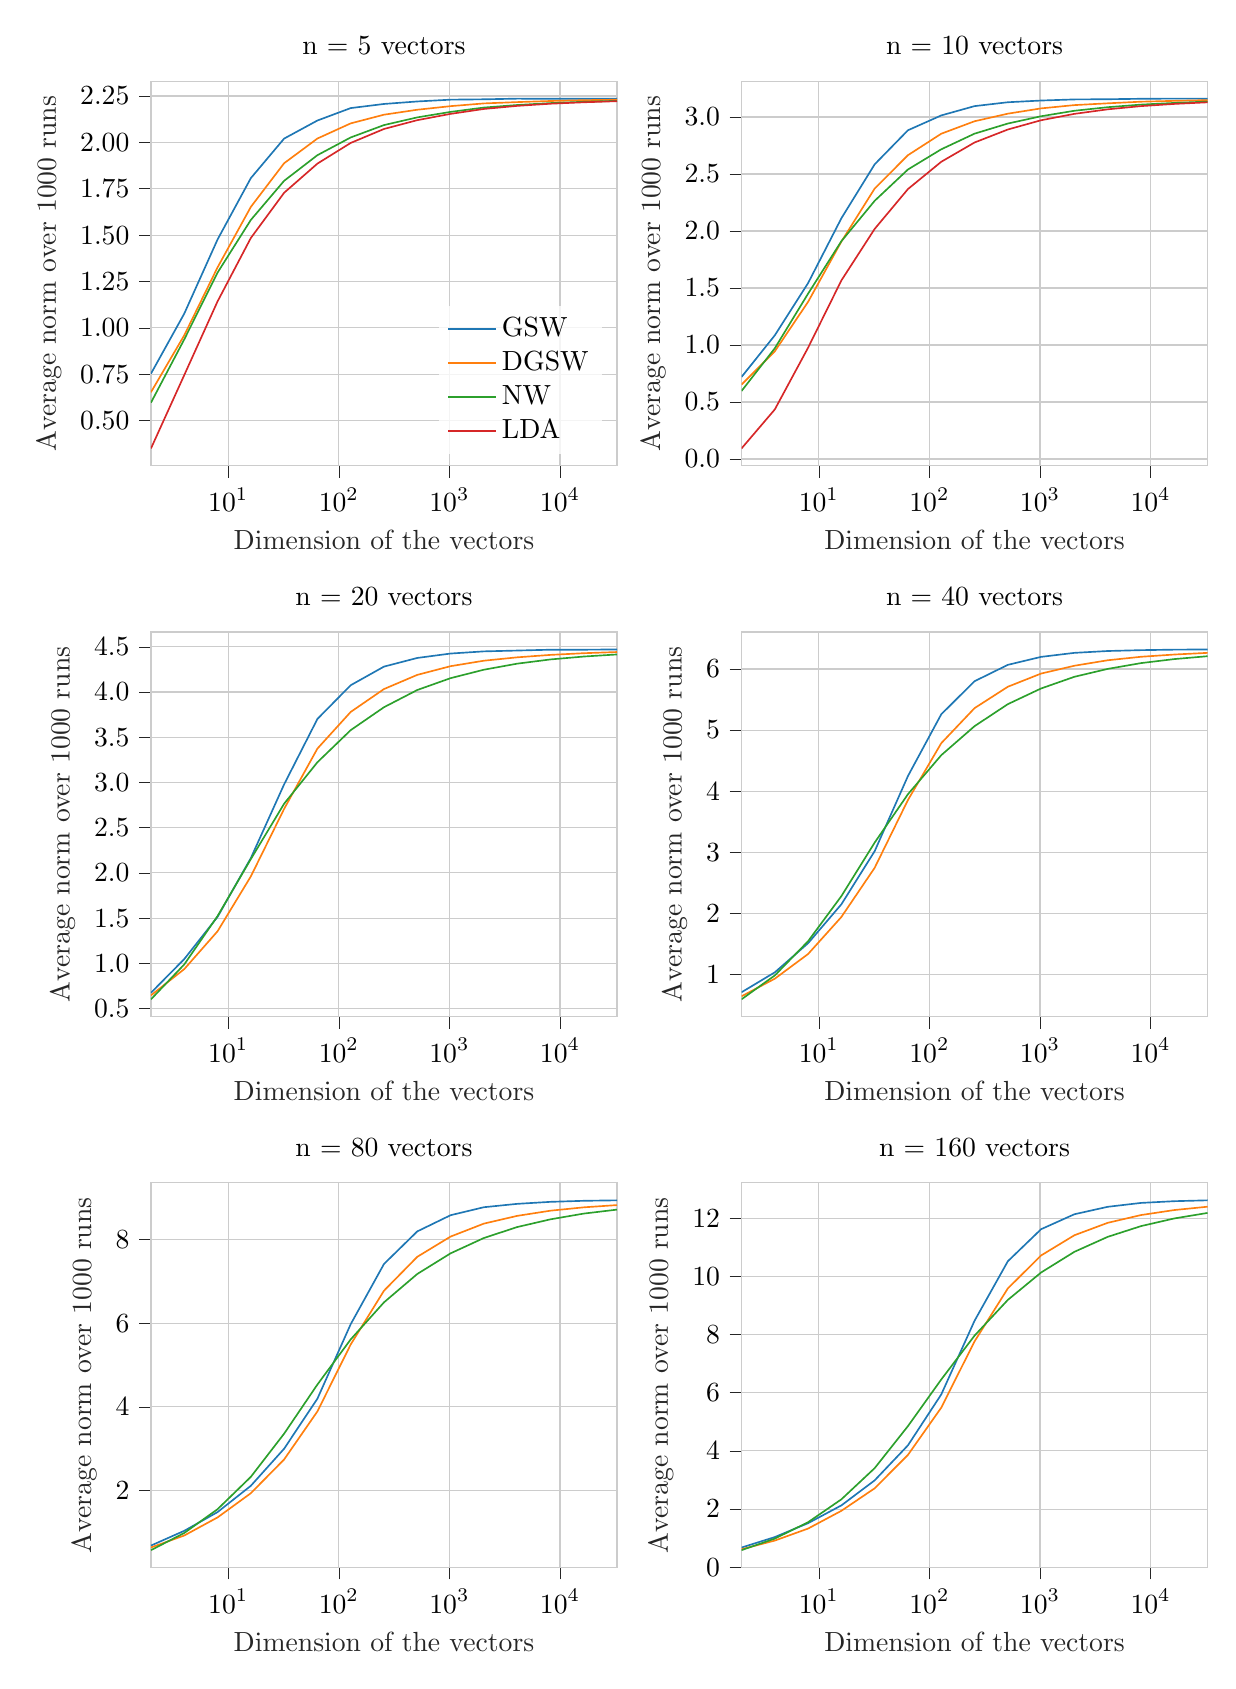
\begin{tikzpicture}

\definecolor{crimson2143940}{RGB}{214,39,40}
\definecolor{darkorange25512714}{RGB}{255,127,14}
\definecolor{darkslategray38}{RGB}{38,38,38}
\definecolor{forestgreen4416044}{RGB}{44,160,44}
\definecolor{lightgray204}{RGB}{204,204,204}
\definecolor{steelblue31119180}{RGB}{31,119,180}

\begin{groupplot}[group style={group size=2 by 3, vertical sep=60 pt, horizontal sep=45 pt,ylabels at=edge left},width=7.5cm]
\nextgroupplot[
axis line style={lightgray204},
legend cell align={left},
legend style={
  fill opacity=0.8,
  draw opacity=1,
  text opacity=1,
  at={(0.97,0.03)},
  anchor=south east,
  draw=none
},
log basis x={10},
tick align=outside,
tick pos=left,
title={n = 5 vectors},
x grid style={lightgray204},
xlabel=\textcolor{darkslategray38}{Dimension of the vectors},
xmajorgrids,
xmin=2, xmax=32768,
xmode=log,
xtick style={color=darkslategray38},
xtick={0.1,1,10,100,1000,10000,100000,1000000},
xticklabels={
  \(\displaystyle 10^{-1}\),
  \(\displaystyle 10^{0}\),
  \(\displaystyle 10^{1}\),
  \(\displaystyle 10^{2}\),
  \(\displaystyle 10^{3}\),
  \(\displaystyle 10^{4}\),
  \(\displaystyle 10^{5}\),
  \(\displaystyle 10^{6}\)
},
y grid style={lightgray204},
ylabel=\textcolor{darkslategray38}{Average norm over 1000 runs},
ymajorgrids,
ymin=0.255696948053937, ymax=2.33025980992646,
ytick style={color=darkslategray38},
ytick={0.25,0.5,0.75,1,1.25,1.5,1.75,2,2.25,2.5},
yticklabels={
  \(\displaystyle 0.25\),
  \(\displaystyle 0.50\),
  \(\displaystyle 0.75\),
  \(\displaystyle 1.00\),
  \(\displaystyle 1.25\),
  \(\displaystyle 1.50\),
  \(\displaystyle 1.75\),
  \(\displaystyle 2.00\),
  \(\displaystyle 2.25\),
  \(\displaystyle 2.50\)
}
]
\addplot [semithick, steelblue31119180]
table {%
2 0.753302962920892
4 1.07681391443778
8 1.4763954247701
16 1.80725844448935
32 2.02042838660354
64 2.11781952489226
128 2.18489156937866
256 2.20707153165223
512 2.22054362484896
1024 2.23025365321102
2048 2.23216903772218
4096 2.23568311872374
8192 2.23507403470857
16384 2.23539183545824
32768 2.23596149802316
};
\addlegendentry{GSW}
\addplot [semithick, darkorange25512714]
table {%
2 0.653162873456715
4 0.960111880506343
8 1.32606485827386
16 1.65204584008202
32 1.88758371650727
64 2.02075412341854
128 2.10244259433338
256 2.14920423124153
512 2.17593629286911
1024 2.19525986330942
2048 2.21000373172618
4096 2.21710304164254
8192 2.22306141597871
16384 2.2273784820361
32768 2.22996161565451
};
\addlegendentry{DGSW}
\addplot [semithick, forestgreen4416044]
table {%
2 0.596901245083498
4 0.937988113392041
8 1.29787066764492
16 1.58189936647815
32 1.79281083729897
64 1.93095806565725
128 2.02655771755907
256 2.0932556166362
512 2.13472143907975
1024 2.16432819478045
2048 2.18764604712878
4096 2.20139440605893
8192 2.21172406480321
16384 2.21878541132863
32768 2.22385946371601
};
\addlegendentry{NW}
\addplot [semithick, crimson2143940]
table {%
2 0.349995259957233
4 0.745586905456825
8 1.14261938161702
16 1.48448275215293
32 1.72829394412234
64 1.88554075674287
128 1.99697706538675
256 2.07223793651122
512 2.1197049607246
1024 2.15357196582785
2048 2.18013050882434
4096 2.19675426428705
8192 2.20842349777013
16384 2.21612086336389
32768 2.2221087026373
};
\addlegendentry{LDA}

\nextgroupplot[
axis line style={lightgray204},
log basis x={10},
tick align=outside,
tick pos=left,
title={n = 10 vectors},
x grid style={lightgray204},
xlabel=\textcolor{darkslategray38}{Dimension of the vectors},
xmajorgrids,
xmin=2, xmax=32768,
xmode=log,
xtick style={color=darkslategray38},
xtick={0.1,1,10,100,1000,10000,100000,1000000},
xticklabels={
  \(\displaystyle 10^{-1}\),
  \(\displaystyle 10^{0}\),
  \(\displaystyle 10^{1}\),
  \(\displaystyle 10^{2}\),
  \(\displaystyle 10^{3}\),
  \(\displaystyle 10^{4}\),
  \(\displaystyle 10^{5}\),
  \(\displaystyle 10^{6}\)
},
y grid style={lightgray204},
ylabel=\textcolor{darkslategray38}{Average norm over 1000 runs},
ymajorgrids,
ymin=-0.0609178268111194, ymax=3.31530910283758,
ytick style={color=darkslategray38},
ytick={-0.5,0,0.5,1,1.5,2,2.5,3,3.5},
yticklabels={
  \(\displaystyle -0.5\),
  \(\displaystyle 0.0\),
  \(\displaystyle 0.5\),
  \(\displaystyle 1.0\),
  \(\displaystyle 1.5\),
  \(\displaystyle 2.0\),
  \(\displaystyle 2.5\),
  \(\displaystyle 3.0\),
  \(\displaystyle 3.5\)
}
]
\addplot [semithick, steelblue31119180]
table {%
2 0.71963241265429
4 1.0852203581318
8 1.54347285291976
16 2.11220667041569
32 2.58535554904408
64 2.8841554862258
128 3.01430957950078
256 3.09589618460011
512 3.12987144255265
1024 3.14489106503139
2048 3.1546372843504
4096 3.15632542555646
8192 3.16035680486506
16384 3.16184424239901
32768 3.16111602809429
};
\addplot [semithick, darkorange25512714]
table {%
2 0.653023635739611
4 0.944658941343891
8 1.37908041607119
16 1.90795138224728
32 2.37276714076937
64 2.66549921628989
128 2.8538107144215
256 2.96312366169186
512 3.02957148737987
1024 3.07603922251443
2048 3.10483268210492
4096 3.12047536691133
8192 3.13467598479665
16384 3.14208293761345
32768 3.14862969934486
};
\addplot [semithick, forestgreen4416044]
table {%
2 0.596321346498368
4 0.971699620385933
8 1.4508547025876
16 1.91098035267129
32 2.26528563900459
64 2.54012777594714
128 2.71707760163129
256 2.85423640498787
512 2.94312005779241
1024 3.00712232464238
2048 3.05516908913614
4096 3.08640756590161
8192 3.1091390760346
16384 3.12386964383172
32768 3.13561707758784
};
\addplot [semithick, crimson2143940]
table {%
2 0.092547033627458
4 0.434918785181621
8 0.976610159741337
16 1.56668587771316
32 2.01879357092335
64 2.36828749682822
128 2.60759513529195
256 2.77672937305124
512 2.89061888892472
1024 2.97207701997941
2048 3.02794633932224
4096 3.06764244915016
8192 3.09592722200594
16384 3.11519462847434
32768 3.12929651255484
};

\nextgroupplot[
axis line style={lightgray204},
log basis x={10},
tick align=outside,
tick pos=left,
title={n = 20 vectors},
x grid style={lightgray204},
xlabel=\textcolor{darkslategray38}{Dimension of the vectors},
xmajorgrids,
xmin=2, xmax=32768,
xmode=log,
xtick style={color=darkslategray38},
xtick={0.1,1,10,100,1000,10000,100000,1000000},
xticklabels={
  \(\displaystyle 10^{-1}\),
  \(\displaystyle 10^{0}\),
  \(\displaystyle 10^{1}\),
  \(\displaystyle 10^{2}\),
  \(\displaystyle 10^{3}\),
  \(\displaystyle 10^{4}\),
  \(\displaystyle 10^{5}\),
  \(\displaystyle 10^{6}\)
},
y grid style={lightgray204},
ylabel=\textcolor{darkslategray38}{Average norm over 1000 runs},
ymajorgrids,
ymin=0.408743206393034, ymax=4.66441911686359,
ytick style={color=darkslategray38},
ytick={0,0.5,1,1.5,2,2.5,3,3.5,4,4.5,5},
yticklabels={
  \(\displaystyle 0.0\),
  \(\displaystyle 0.5\),
  \(\displaystyle 1.0\),
  \(\displaystyle 1.5\),
  \(\displaystyle 2.0\),
  \(\displaystyle 2.5\),
  \(\displaystyle 3.0\),
  \(\displaystyle 3.5\),
  \(\displaystyle 4.0\),
  \(\displaystyle 4.5\),
  \(\displaystyle 5.0\)
}
]
\addplot [semithick, steelblue31119180]
table {%
2 0.674457963933909
4 1.04721939591112
8 1.51334196021062
16 2.16407948785203
32 2.97932299026144
64 3.70241028487034
128 4.07547726020147
256 4.2814045970973
512 4.37715139205982
1024 4.42581240200165
2048 4.44982528609241
4096 4.45893816702605
8192 4.46815892178249
16384 4.46836502601736
32768 4.47097930275129
};
\addplot [semithick, darkorange25512714]
table {%
2 0.646118433717414
4 0.936347023218119
8 1.35455384406888
16 1.96143586997306
32 2.70827514261334
64 3.37466064522229
128 3.78014229185702
256 4.03323610473627
512 4.18994134955916
1024 4.28609076198406
2048 4.34664123806133
4096 4.38389244256932
8192 4.41095798111683
16384 4.42959162322253
32768 4.44258702017551
};
\addplot [semithick, forestgreen4416044]
table {%
2 0.602183020505332
4 0.987884539608238
8 1.52289464398874
16 2.15273966806521
32 2.76517796306832
64 3.22376058299526
128 3.57882194611212
256 3.83231114293771
512 4.02270215094316
1024 4.15362303269105
2048 4.24694839516339
4096 4.31392000605389
8192 4.3606381192735
16384 4.3926989817818
32768 4.41575040710829
};

\nextgroupplot[
axis line style={lightgray204},
log basis x={10},
tick align=outside,
tick pos=left,
title={n = 40 vectors},
x grid style={lightgray204},
xlabel=\textcolor{darkslategray38}{Dimension of the vectors},
xmajorgrids,
xmin=2, xmax=32768,
xmode=log,
xtick style={color=darkslategray38},
xtick={0.1,1,10,100,1000,10000,100000,1000000},
xticklabels={
  \(\displaystyle 10^{-1}\),
  \(\displaystyle 10^{0}\),
  \(\displaystyle 10^{1}\),
  \(\displaystyle 10^{2}\),
  \(\displaystyle 10^{3}\),
  \(\displaystyle 10^{4}\),
  \(\displaystyle 10^{5}\),
  \(\displaystyle 10^{6}\)
},
y grid style={lightgray204},
ylabel=\textcolor{darkslategray38}{Average norm over 1000 runs},
ymajorgrids,
ymin=0.30568849651664, ymax=6.6060569328654,
ytick style={color=darkslategray38},
ytick={0,1,2,3,4,5,6,7},
yticklabels={
  \(\displaystyle 0\),
  \(\displaystyle 1\),
  \(\displaystyle 2\),
  \(\displaystyle 3\),
  \(\displaystyle 4\),
  \(\displaystyle 5\),
  \(\displaystyle 6\),
  \(\displaystyle 7\)
}
]
\addplot [semithick, steelblue31119180]
table {%
2 0.7073859014731
4 1.03359385099533
8 1.51048699418052
16 2.14766462101957
32 3.01767405188754
64 4.24814758768958
128 5.25851890369424
256 5.7997681249829
512 6.06775715531927
1024 6.1985481457907
2048 6.26409079288542
4096 6.29444903724707
8192 6.30844847384504
16384 6.31666332329645
32768 6.319676549395
};
\addplot [semithick, darkorange25512714]
table {%
2 0.641314074076739
4 0.929528526784163
8 1.33367707316419
16 1.9401523487888
32 2.74534936687179
64 3.85536693997492
128 4.78531477399343
256 5.35900599307197
512 5.7092250845821
1024 5.92523021627011
2048 6.05328064708366
4096 6.14291076110132
8192 6.19987127616011
16384 6.23675627925348
32768 6.26416030096064
};
\addplot [semithick, forestgreen4416044]
table {%
2 0.592068879987038
4 0.982881312602817
8 1.54359897418113
16 2.28181026276854
32 3.15797607785146
64 3.9503195952634
128 4.58880477030826
256 5.06400001468298
512 5.42433688040962
1024 5.68134104010232
2048 5.87223706681866
4096 6.00148025003473
8192 6.09635407400215
16384 6.16208383923135
32768 6.20927821628785
};

\nextgroupplot[
axis line style={lightgray204},
log basis x={10},
tick align=outside,
tick pos=left,
title={n = 80 vectors},
x grid style={lightgray204},
xlabel=\textcolor{darkslategray38}{Dimension of the vectors},
xmajorgrids,
xmin=2, xmax=32768,
xmode=log,
xtick style={color=darkslategray38},
xtick={0.1,1,10,100,1000,10000,100000,1000000},
xticklabels={
  \(\displaystyle 10^{-1}\),
  \(\displaystyle 10^{0}\),
  \(\displaystyle 10^{1}\),
  \(\displaystyle 10^{2}\),
  \(\displaystyle 10^{3}\),
  \(\displaystyle 10^{4}\),
  \(\displaystyle 10^{5}\),
  \(\displaystyle 10^{6}\)
},
y grid style={lightgray204},
ylabel=\textcolor{darkslategray38}{Average norm over 1000 runs},
ymajorgrids,
ymin=0.155886461988915, ymax=9.35246897447473,
ytick style={color=darkslategray38},
ytick={0,2,4,6,8,10},
yticklabels={
  \(\displaystyle 0\),
  \(\displaystyle 2\),
  \(\displaystyle 4\),
  \(\displaystyle 6\),
  \(\displaystyle 8\),
  \(\displaystyle 10\)
}
]
\addplot [semithick, steelblue31119180]
table {%
2 0.683760238825937
4 1.03613939665838
8 1.48356466912655
16 2.11217494147394
32 2.99863207064923
64 4.1942216226175
128 5.97474281927574
256 7.41373929949157
512 8.19193225448914
1024 8.57858665204354
2048 8.76972182635999
4096 8.85010278865581
8192 8.89816984981962
16384 8.9231193646131
32768 8.93444249663447
};
\addplot [semithick, darkorange25512714]
table {%
2 0.638395447693833
4 0.924136569391656
8 1.35624922067856
16 1.93506269665922
32 2.74145041015036
64 3.89007169744495
128 5.48975362235344
256 6.77472656470111
512 7.58439011501749
1024 8.06800436434704
2048 8.37781115757593
4096 8.56284123893403
8192 8.68674364130783
16384 8.76692545958742
32768 8.82078073208617
};
\addplot [semithick, forestgreen4416044]
table {%
2 0.573912939829179
4 0.984302655726752
8 1.55276160623233
16 2.32616417712536
32 3.35815230409654
64 4.53216841909841
128 5.61062947324815
256 6.49654377935948
512 7.17432371805998
1024 7.66730217351666
2048 8.03377596554526
4096 8.29547032826648
8192 8.48024687974597
16384 8.61747085670411
32768 8.71224200913121
};

\nextgroupplot[
axis line style={lightgray204},
log basis x={10},
tick align=outside,
tick pos=left,
title={n = 160 vectors},
x grid style={lightgray204},
xlabel=\textcolor{darkslategray38}{Dimension of the vectors},
xmajorgrids,
xmin=2, xmax=32768,
xmode=log,
xtick style={color=darkslategray38},
xtick={0.1,1,10,100,1000,10000,100000,1000000},
xticklabels={
  \(\displaystyle 10^{-1}\),
  \(\displaystyle 10^{0}\),
  \(\displaystyle 10^{1}\),
  \(\displaystyle 10^{2}\),
  \(\displaystyle 10^{3}\),
  \(\displaystyle 10^{4}\),
  \(\displaystyle 10^{5}\),
  \(\displaystyle 10^{6}\)
},
y grid style={lightgray204},
ylabel=\textcolor{darkslategray38}{Average norm over 1000 runs},
ymajorgrids,
ymin=-0.0143503237300027, ymax=13.2184230140548,
ytick style={color=darkslategray38},
ytick={-2,0,2,4,6,8,10,12,14},
yticklabels={
  \(\displaystyle -2\),
  \(\displaystyle 0\),
  \(\displaystyle 2\),
  \(\displaystyle 4\),
  \(\displaystyle 6\),
  \(\displaystyle 8\),
  \(\displaystyle 10\),
  \(\displaystyle 12\),
  \(\displaystyle 14\)
}
]
\addplot [semithick, steelblue31119180]
table {%
2 0.677734491084107
4 1.03692346319212
8 1.51548028925789
16 2.12666410723212
32 2.98799796527184
64 4.19268288057004
128 5.94184034077358
256 8.47546085642666
512 10.5212953294629
1024 11.6242549740486
2048 12.1381529989464
4096 12.3936535409674
8192 12.527566850188
16384 12.587227776337
32768 12.6169333168828
};
\addplot [semithick, darkorange25512714]
table {%
2 0.618723289188252
4 0.916816081443127
8 1.32978007350891
16 1.94007905555627
32 2.71431115482378
64 3.86411830063603
128 5.48716255187505
256 7.76576014170662
512 9.5871199706287
1024 10.7213626308633
2048 11.4160004858233
4096 11.8430807284886
8192 12.1099756556854
16384 12.2823209792783
32768 12.3974280294337
};
\addplot [semithick, forestgreen4416044]
table {%
2 0.587139373442035
4 0.984508476764333
8 1.54893945050985
16 2.33514986712373
32 3.4074787795939
64 4.85338331786451
128 6.45637641393051
256 7.96357273871975
512 9.19213944973677
1024 10.1358495229114
2048 10.8462322478091
4096 11.360379445379
8192 11.7300352309326
16384 11.9935983794131
32768 12.1834728057053
};
\end{groupplot}\end{tikzpicture}

\caption{Results of experiment 1 from section \ref{how_good_at_minimizing_disc}: comparison of different norm of vector of imbalances minimizing algorithms for $n=5,10,20,40,80,160$ vectors of dimension between $2$ and $2^{15}$. Results were averaged over 1000 runs.}\label{output_disc}
\end{figure}
Our results are visible in figure \ref{output_disc}. We can see that GSW actually gives the worst results in terms of minimization of the norm of the vector of imbalances, but that when the dimension of the vector grows all methods seem to give similar results asymptotically. Note that we cannot say that the naive walk is just a better minimizing algorithm for this problem as these results would probably be different if we modified the distribution of input vectors.

\subsubsection{Experiment 2}
While the GSW obviously has some other desirable properties, there should be input vector sets on which the GSW returns shorter vector of imbalances on average than the naive walk. If the vectors aren't shuffled before the naive walk, it is trivial to find a set on which the GSW produces shorter vectors of imbalances. If they are, it isn't as trivial but it still isn't too hard. For example let's run the GSW and the naive walk on the set containing 100 copies of both $v_1$ and $v_2$ where $$v_1=\begin{pmatrix}1\\0\end{pmatrix},\quad v_2=\begin{pmatrix}\frac{10}{\sqrt{2}}\\ \frac{10}{\sqrt{2}}\end{pmatrix}.$$
We will record the norm of the resulting vector of imbalances for 100 runs of each walk and observe the average.
\subsubsection{Results 2}
The resulting average norm is exactly $0$ for the GSW and $3.47$ for the naive walk, showing that the naive walk can yield much higher norms when the input vectors are less well-behaved. Indeed, the naive walk doesn't use the knowledge of the full input vector set like the GSW does and thus fails to balance this set well.

\subsection{Does translation of the input vectors have an effect on the balance of the assignment ?}\label{trans_balance}
By \textit{balance of the assignment}, we mean the absolute difference between the number of 1s and -1s. An assignment is perfectly balanced if its sum is 0, that is the groups produced by the assignment have equal size.

If our initial group of vector is centered around \textbf{0}, we would expect that translating it away will force it to have a greater balance between -1s and 1s in order to balance the translation part added to each vector.

\subsubsection{Experiment}
We sample 200 input vectors from the ball of radius 1 in dimension 200. We then run the GSW and DGSW 100 times each on those vector translated by some random norm 1 vector multiplied by some factor. We use the factors 0,1,2,5 and 10 and compare the results.

\subsubsection{Results}
\begin{table}[h!]
\centering
\caption{Results of our experiment from section \ref{trans_balance} on the balance of assignments depending on how much the vectors are translated. The numbers shown are the average absolute value of the sums of output vectors. A smaller number indicates that the assignment is more balanced, that is the number of 1's and -1's are closer.}
\begin{tabular}{l|llllll}
 Factor & 0 & 1  & 2 & 5 & 10  \\
\hline
GSW  & 9.7 & 0.96 & 0.46 & 0.1 & 0.06 \\
DGSW & 44.5 & 1.78 & 0.32 & 0.08 & 0.04
\end{tabular}
\label{balance_when_translated}\end{table}
Results are available in table \ref{balance_when_translated}. We can see that indeed the further away from 0 our input vectors are translated the more balanced the assignments are, as expected. It's interesting to notice that assignments from the DGSW are way less balanced than with the GSW. I currently do not have any hypothesis on why that is.

These experiments make us want to try to build a variant of GSW that can have a balance parameter thanks to the balancing properties of translation. That is what we try in the following experiment.

\subsection{Can we add a parameter to balance assignments ?}\label{balance_parameter}
Inspired by section \ref{trans_balance}, we propose a slight modification of the GSW that pushes toward balanced assignments. The idea is to add a coordinate to the input vector and give more or less importance to that coordinate similarly to how the balance-robustness tradeoff is implemented in \cite{harshaw2019balancing}, except here we implement a tradeoff between assignment balance and norm of the vector of imbalances.

Given input vectors $\textbf{v}_1,\dots,\textbf{v}_n\in\mathbb{R}^d$ and a parameter $\mu\in[0,1]$, we define $\textbf{w}_1,\dots,\textbf{w}_n\in\mathbb{R}^{d+1}$ as $$\textbf{w}_i=\begin{pmatrix}\sqrt{1-\mu}\textbf{v}_i \\ \sqrt{\mu}\end{pmatrix}.$$ This way the $\textbf{w}_i$'s have similar norm to the $\textbf{v}_i$'s, but it is possible that a different normalization depending on the norm of the $\textbf{v}_i$'s could be better. We then run the GSW on the $\textbf{w}_i$'s and use the output assignment on the $\textbf{v}_i$'s. Choosing $\mu=0$ is equivalent to doing the classical GSW algorithm, while using $\mu=1$ is equal to forcing maximum balance. We run experiments to determine how much balance in the assignment we gain and how much further from \textbf{0} our output is for different $\mu$'s.

\subsubsection{Experiment}
We use our construction from the previous paragraph to compute an assignment on the $\textbf{w}_i$'s using GSW or DGSW, then record how balanced this assignment is, and how the norm of its vector of imabalances on the original $\textbf{v}_i$'s varies. We also program the fixed size GSW described in \cite{harshaw2019balancing} and compare it with our balancing method. We use $n$ vectors sampled from the ball of radius 1 in dimension $n$ for $n=100$ and $\mu\in\{0,0.001,0.01,0.1,0.25,0.5,0.75,0.9,0.99,0.999,1\}$. The results presented are averaged over 1000 runs.

\subsubsection{Results}
\begin{table}[h!]
\centering
\caption{Results of our experiment on the balance of assignments with our new balance-norm of the vector of imbalances tradeoff design. The balance measure shown (lines starting with AB for average balance) are the average absolute value of the sums of assignment vectors. The norm of the vector of imbalances numbers shown (lines starting with AN for average norm of imbalance) are the norms of the sum of $\textbf{v}_i\cdot \textbf{z}_i$, $\textbf{z}$ being the assignment produced by GSW or DGSW for the $\textbf{w}_i$'s. %For the last column, we used the fixed size GSW design from \cite{harshaw2019balancing} rather than what is described in section\ref{balance_parameter}. 
The D at the end of the last two lines indicates that in this case, the deterministic GSW algorithms was used.\\
A smaller balance measure indicates that the assignment has a more balanced assignment, that is the number of 1s and -1s are closer. A smaller norm of imbalances measure indicates that the vectors are better balanced among the groups, that is the sum of each coordinate is closer to be the same in each group. FSD references the fixed size design from \cite{harshaw2019balancing}, which was used for the rightmost column in order to compare it with what is described in section \ref{balance_parameter}.}
\begin{tabular}{l|llllllllllll}
 $\mu$ &0&0.001&0.01&0.1&0.25&0.5&0.75&0.9&0.99&0.999&1&FSD\\
\hline
AB&8.09&6.25&4.16&1.9&1.11&0.58&0.27&0.11&0.01&0.002&0&0 \\
AN&5.26&5.28&5.27&5.31&5.34&5.32&5.34&5.33&5.33&5.34&9.92&5.32\\
ABD&20.58&18.7&11.91&3.89&2.04&0.99&0.33&0.12&0.02&0.002&0&0\\
AND&4.86&4.84&4.78&4.82&4.89&4.94&4.99&5.0&5.0&5.0&9.85&5.01
\end{tabular}
\label{balance_tradeoff_results}
\end{table}


We can see that we can massively increase assignment balance without making the norm of the vector of imbalances much larger. For $\mu=0.999$ for example, it is very likely that an assignment is exactly balanced and thus this variant of the algorithm can provide balanced GSW assignments with high probability while keeping most properties of the classical GSW, as opposed to the balanced variant described in \cite{harshaw2019balancing}, for which we don't know if some of the original properties still hold. %The high probability comes from the subgaussianity bound.

%\subsection{What else can we control by adding coordinates ?}
%We could think of a design where we want several subgroups, potentially of only 2 vectors per subgroup, to be balanced. We could then add a coordinate for each subgroup and put the same number on that coordinate for each member of the subgroup, while putting 0 for every vector that isn't in the subgroup. This would push towards balancing within any subgroup we want, and could be done via some parametering similar to what was done in section \ref{balance_parameter}. 
%
%Similarly, if we want 2 vectors to be in the same group because of some previous knowledge about the input vector set, we could add a dimension and assign some number $x$ and $-x$ to these vectors in that new dimension while giving 0 to every other vector in that dimension.
%
%Note that if we want to force two vectors $\textbf{v}_i,\textbf{v}_j$ to be in the same or the opposite group, we could remove them from the input and add their sum or difference respectively. Then, looking at what group was assigned to the sum or difference we could get an assignment for the actual input vectors (including $\textbf{v}_i$ and $\textbf{v}_j$).
%
%%Adding dimensions could be used to translate knowledge about the vector set into usable information for the algorithm.
%Depending on the type of constraints we have on our assignment, or if we want to modify the distribution or the property of an assignment, there is a chance that this can be done by adding coordinates to the input vectors. Thus, for specific applications where the GSW is used, this technique could be useful.



%\subsection{Does norm affect the balance of the assignment ?}
%We would expect norms not to affect the balance of the assignment, as multiplying every input vector by the same factor should mean the algorithm runs similarly.

\subsection{Does the norm of a vector affect when it is colored ?}\label{norm_affect_when}
The expected heuristic would have been that bigger vectors are colored earlier and the algorithm then colors the smaller ones to balance the longer ones in order to minimize the norm of the vector of imbalances, as that is what we'd instinctively do. It turns out that the algorithm actually does the reverse and colors the smaller vectors earlier than the bigger ones.

We performed two experiments to observe this behavior. In both experiments, we have vectors $\textbf{v}_1,\dots,\textbf{v}_{200}$ of increasing norm and observe how close the coloring order is to $\mathcal{R}=\{200,199,$\dots$,1\}$. To do so, if $\mathcal{O}$ is the observed order, we look at the quantity 
\begin{equation}
\Delta_{o}=\sum_{i=1}^{200}|\mathcal{R}_i-\mathcal{O}_i|.
\label{orderdistance}
\end{equation}
The smaller it is, the closer the 2 orders are. For each of the two experiments below, we ran the GSW 100 times and the deterministic GSW (DGSW) 100 times and recorded $\Delta_o$.

\subsubsection{Experiment 1}
We sampled 200 vectors $\textbf{v}_1,\dots,\textbf{v}_{200}$ in the ball of radius 1 of dimension 200. For each $\textbf{v}_i$, we replaced it by $i\cdot \textbf{v}_i/\|\textbf{v}_i\|$ so that $\|\textbf{v}_i\|=i$ for each vector. We call this vector set the incrementally growing norm set (IGN).


\subsubsection{Experiment 2}
We sampled 200 vectors $\textbf{v}_1,\dots,\textbf{v}_{200}$ in the ball of radius 1 of dimension 200. For each $\textbf{v}_i$, we replaced it by $X_i\cdot \textbf{v}_i/\|\textbf{v}_i\|$ so that $\|\textbf{v}_i\|=X_i$ for each vector, where $X_i=1 + 199\cdot\mathds{1}_{i<n/2}$. We call this vector set the two group set (2G).

\subsubsection{Results}\label{results_norm_affect_when}
We also ran the same experiments with 200 vectors of constant norm 1 as a comparison, which we call the all equal norm set (AEN). The results are summarized in table \ref{norm_when_colored}.
\begin{table}[h!]
\centering
\caption{Results of our experiments on the moment of coloring depending on the norm of the vectors. The numbers shown are the $\Delta_o$ as defined in equation \ref{orderdistance}.}
\begin{tabular}{l|lll}
& IGN & 2G & AEN  \\
\hline
GSW & 18664.4 & 19997.32 & 13607.06 \\
DGSW & 18641.6 & 19996.16 & 13431.68
\end{tabular}
\label{norm_when_colored}
\end{table}

We can see that the vector orders are actually further away from $\mathcal{R}$ than the random orders produced with constant vectors, which means that bigger vectors actually get colored later in the process. Additionally, the DGSW doesn't seem to yield significantly different results. While this is not what we expected upon a first glance at the problem, this behavior actually makes sense, because if we multiply $\textbf{v}_i$ by $\mu%\textbf{v}_i
$, it's corresponding coordinate in $\textbf{u}_t$ is going to be divided by $\mu$, thus it will move less towards the facet of the hypercube corresponding to the color of $\textbf{v}_i$ and thus be colored later than the shorter vectors.

This motivates us to try to find a variant of the algorithm that would color bigger vectors earlier and thus yield shorter vector of imbalances on an input such as $\{\textbf{v},\textbf{v},\textbf{v},3\textbf{v}\}$ for some $\textbf{v}\in\mathbb{R}^d$ and an arbitrary $d\in\mathbb{N}$. One way would be to choose the pivot through some smart condition or to choose another feasible $\textbf{u}_t$ than the default least square solution with minimal norm, as in that specific adversarial example there are an infinite number of valid $\textbf{u}_t$, some of which solve our problem in one step with a perfectly balanced groups.

One such idea is to force the pivot to be the largest norm vector, and then, when $\textbf{v}_\perp=\textbf{0}$, to select $\textbf{u}_t$ through lasso regression with a very small alpha ($\alpha=10^{-32}$ for example) in order to ensure that the smallest possible number of coordinates are nonzero, and finally to select $\delta_t$ by taking it to be of the same sign as the coordinate of $x$ corresponding to the pivot (or randomly if that coordinate is 0). This variant solves the issue mentioned in the previous paragraph but trades a lot of randomness for some additional complexity in the process, so there probably exists some different additional constraint to add when computing $\textbf{u}_t$ in colinear cases that could work even better.

%Another variant that works but only in this trivial example and not in slightly more complicated examples with for examples 2 groups of vectors is to just force the largest alive vector to be the pivot at every step. This is just a product of the exact solution of the least squares we're choosing as there are infinitely many that wouldn't work. This doesn't work for slightly more convoluted adversarial cases and is just a product of our exact implementation.

A second variant that might help is to do quadratic programming instead of simple least squares when $\textbf{v}_\perp(t)=\textbf{0}$. This way, we can force the quadratic program to minimize both $\|\textbf{Bu}_t\|^2$ but also $\|\textbf{u}_t\|^2$. This could be achieved by adding a line of 1's to the matrix $\textbf{B}$ containing all input vectors as column, and adding as conditions that the chosen $\textbf{u}_t$ must have a 1 in the pivot coordinate and 0's in already colored coordinates, similarly to the conditions in the original GSW system of equation. Then if the $\textbf{u}_t$ chosen through this quadratic program doesn't yield $\textbf{Bu}_t=\textbf{0}$, we discard it and compute $\textbf{u}_t$ through the usual method as the modification would then interfere with the normal properties of the GSW instead of just improving it by adding constraints when there are an infinite number of optimal solutions. This technique coupled with choosing the longest alive vector as pivot actually solves adversarial cases similar to those mentioned three paragraphs ago, as well as more complicated ones such as $\{\textbf{v},\textbf{v},\textbf{v},3\textbf{v},\textbf{w},\textbf{w},2\textbf{w}\}$, and doesn't modify the behavior of the algorithm when $\textbf{v}^\perp(t)\not=\textbf{0}$. The only small issue is that the matrix $\textbf{B}^T\textbf{B}$ then needs to be regularized by adding some very small constant times the identity or it isn't strictly positive definite, which is necessary for our quadratic program solver.

A third potential method would be to again do quadratic programming, but this time minimize $|(|u|-1)|$ or $(|u|-1)^2$ in addition to $\|\textbf{Bu}\|$, with the same constraints as previously. Despite not being a quadratic or linear function, absolute value in the objective function can be included, it is just necessary to transform it into linear constraints and additional variables, which is a common linear programming trick. This technique would function without forcing a specific pivot and seems thus superior to the previous one, but I didn't have time to program it and test it to make sure that my intuition is indeed correct.

This last variant seems interesting as it intuitively makes sense to color as much as possible in the early steps, as we have more degrees of freedom during these steps. I have not been able to find a situation where that seemed worse than the classical GSW so far.

Another interesting experiment in the same vein would be to check if these results change with the dimension.

%\subsection{What affects when a vector is colored other than the norm ?}

\subsection{Do longer vectors stay pivot for longer ?}\label{longer_vec_pivot_longer}
As longer vectors are colored later in the algorithm on average, one could think that they're staying as the pivot for longer. To test this hypothesis we design the following experiment.
\subsubsection{Experiment}
We sample 200 vectors of norm 1 in dimension 200 and multiply 100 of them by 200 (G1 with norm 1, G2 with norm 200). We then run the GSW 100 times with all these vectors as input and record for how long vectors of different norms (1 and 200) stay pivot once they become pivot. We call this measure the \textbf{ALOSAP} (average length of stay at pivot), and it is measured in number of while loop steps.
\subsubsection{Results}
\begin{table}[h!]
\centering
\caption{Results of our experiments  from section \ref{longer_vec_pivot_longer} on whether long and short vectors stay for longer as the pivot. Results are averaged across groups from 100 runs.}
\begin{tabular}{l|ll}
 &ALOSAP G1&ALOSAP G2\\
\hline
GSW&6.101&2.281\\
DGSW&5.989&2.277
\end{tabular}
\label{pivot_longer}
\end{table}

Results are visible in table \ref{pivot_longer}. We see that shorter vectors tend to stay pivot for much longer than their longer counterparts. This could be explained by the fact that, as seen in section \ref{norm_affect_when}, longer vectors are colored later. This means that in the later part of a GSW run, most alive elements are in the second group and will thus have similar scale and color each other, whereas in the early steps of a run short vectors are colored by any pivot, and thus short vectors would be mostly chosen as pivot at the beginnning of a run of the GSW. % so longer vectors rarely get colored by a small vector pivot, but shorter vectors do get colored while the longer vectors are pivot.

It would be interesting to confirm or deny that hypothesis with another experiment looking at a more detailed distribution of the colorings and pivots, but we didn't have the time to perform something like that.

\subsection{Can we force bigger vectors to be colored earlier ?}\label{bigger_earlier}
Another technique that we could use would be to modify the choice of the direction. Currently, the bigger a vector is the later in the process it will be colored. 

One could multiply the computed direction in each of its coordinate by the norm of the vector corresponding to that coordinate, or the squared norm. That would be a way of trying to compensate for the update coordinates of bigger vectors being smaller. This would remove the orthogonality of updates, but it doesn't mean that the assignment doesn't balance the vectors, even though we would expect the vector of imbalances obtained via this method to be somewhat longer still.

We also study how that affects the order of the coloring in experiments similar to those done in subsection \ref{norm_affect_when}.
\subsubsection{Experiment 1}\label{bigger_earlier_exp1}
We sample 100 points from the ball of radius 1 in dimension $d=2$ and run the classical GSW, as well as the two variant described in the current section 100 times each. We plot all vectors of imbalances obtained this way to see how these modifications affected the algorithm.
\subsubsection{Experiment 2}\label{bigger_earlier_exp2}
We sample vectors similarly to the experiments performed in section \ref{norm_affect_when} and measure similarly how close the coloring order is to the order $\mathcal{R}=\{200,199,$\dots$,1\}$.
\subsubsection{Results}
\begin{figure}[h!]
% This file was created with tikzplotlib v0.10.1.
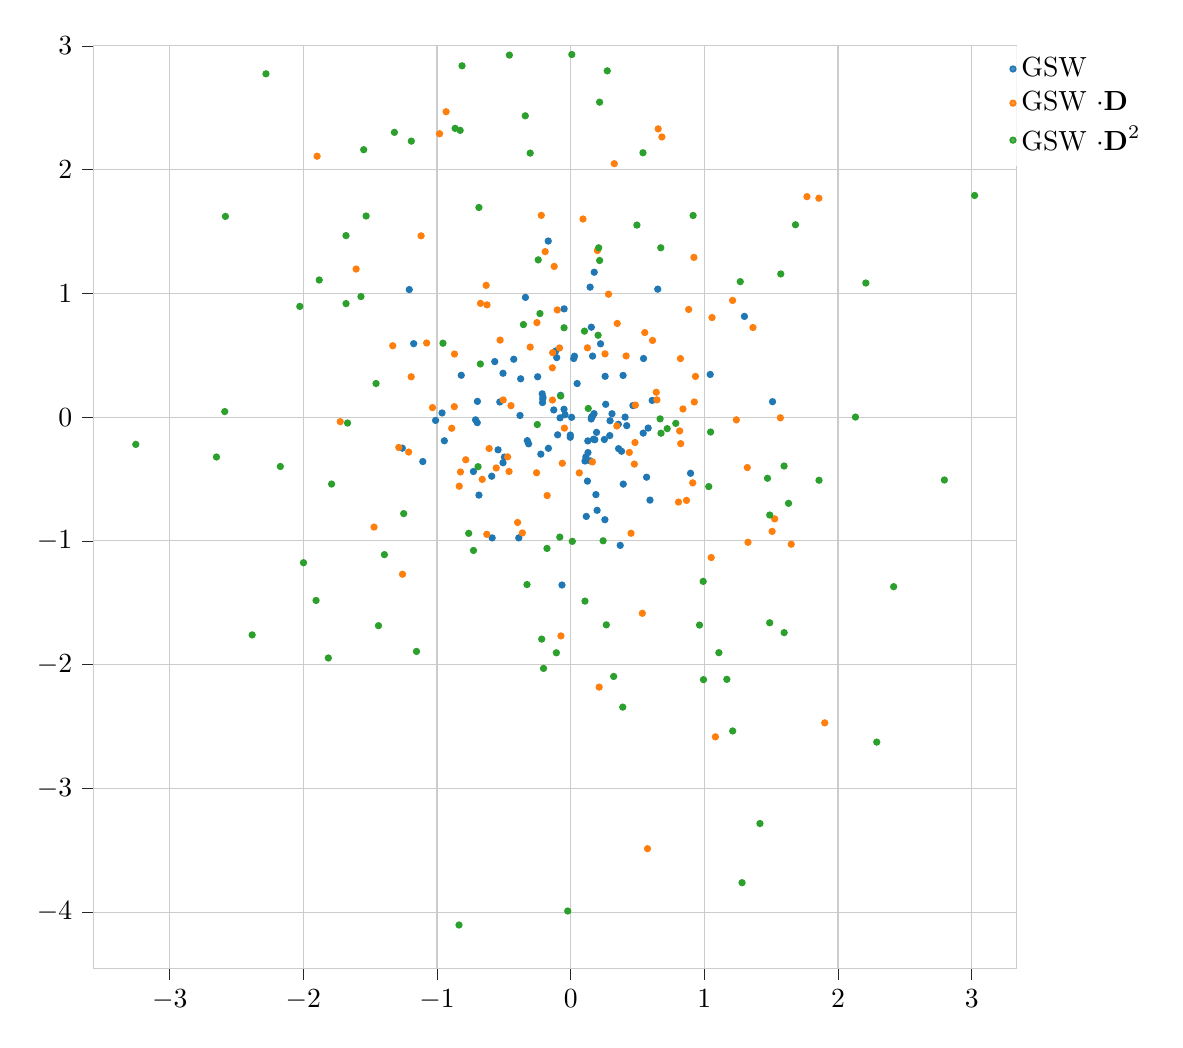
\begin{tikzpicture}

\definecolor{darkorange25512714}{RGB}{255,127,14}
\definecolor{darkslategray38}{RGB}{38,38,38}
\definecolor{forestgreen4416044}{RGB}{44,160,44}
\definecolor{lightgray204}{RGB}{204,204,204}
\definecolor{steelblue31119180}{RGB}{31,119,180}

\begin{axis}[
width=13.3cm,
height=13.3cm,
axis line style={lightgray204},
legend cell align={left},
legend style={fill opacity=0.8, draw opacity=1, text opacity=1, at={(1.15,1)}, draw=none},
tick align=outside,
tick pos=left,
x grid style={lightgray204},
xmajorgrids,
xmin=-3.56756457944001, xmax=3.33550421843633,
xtick style={color=darkslategray38},
y grid style={lightgray204},
ymajorgrids,
ymin=-4.45510115448664, ymax=3,
ytick style={color=darkslategray38}
]
\addplot [semithick, steelblue31119180, mark=*, mark size=1, mark options={solid}, only marks]
table {%
-0.568269744765375 0.448494544232229
0.113334582503312 -0.321977608063704
-0.506591520785814 -0.368735924790621
0.129013449296536 -0.286766602489465
-1.01102124579515 -0.0267085428249436
0.163597463285025 0.492966584154245
0.370300171168456 -1.03628925819198
0.157153523088212 0.00284093356630044
-0.686717053099526 -0.630155819679375
0.022440805265466 0.473342089734238
0.125167836299408 -0.517129827106344
1.50994624796006 0.124486775513971
-0.0796834643564927 -0.00604978227449593
-0.0761451435239965 0.176152759265025
-0.207579890787228 0.160221902740941
0.1757555351185 1.17054338770843
-0.0492412737395029 0.874547435537592
-0.388720191368295 -0.975833570622775
0.356240058069854 -0.0580788390207754
0.292104995004017 -0.149301350114433
-0.166974896097364 -0.251923999783568
-0.962463428668065 0.0337816031440061
0.29444181091756 -0.0291836174820228
-0.324592371336185 -0.190334860209362
-0.211014625547082 0.117539325508916
-0.379239861767305 0.0135325527432488
0.170288294111926 -0.178805814215384
-0.11247570674151 0.534190639266237
0.153390564897879 -0.015105289630833
0.251617947686654 -0.180794663051696
-0.126762839356116 0.0579052555527655
-0.53051229342717 0.122330784704325
0.391985519927001 0.336735115009189
-0.727738839594128 -0.439376686741493
0.406977044037613 0.000114998938818722
-0.699148169741176 -0.0446530801523248
-0.314902255983084 -0.215777631932432
-0.247391044464105 0.325933057591272
0.257437328121716 0.32970989650549
-1.10658037268823 -0.359037992108968
-0.168159522276014 1.42243969790967
0.223344735800472 0.592127258123742
-0.587686989755964 -0.97585983583471
1.04369251331888 0.344584219433935
-0.945328947742684 -0.191296968807523
0.180412424597129 -0.18238321967837
0.5424324390914 -0.129228412895273
-0.0034750457491404 -0.162840990491827
-0.065317248617454 -1.35653147257776
-0.591150316193277 -0.477529446103391
0.60936337053801 0.134807340647683
0.651004950182169 1.03378679192775
0.12791039671738 -0.192185357527169
0.145179566188723 1.05007200801685
-0.374410010819939 0.309537952605789
0.39323101551049 -0.541235314266358
-0.209037455254464 0.146561852131287
0.567619688645187 -0.485442024090579
-0.818780808488631 0.337997453216531
0.380223616388464 -0.275870011498392
-0.496034210478598 -0.323170214690077
0.255649204729229 -0.828846985316821
-0.506496916391257 0.354265329433723
-0.697905823124344 0.126937346952347
0.0482265737342629 0.271077640218718
0.116479376123441 -0.802373074831354
0.261692617445017 0.103592229357728
-1.25989162894926 -0.250936805735669
0.147036501610927 -0.353597416280502
-0.543419078541173 -0.264276485274836
-0.21339124757108 0.188346750463003
0.193308002303774 -0.123209072808406
-0.097846026213097 -0.143087186128311
1.29966286852325 0.813716524159657
-0.711898454065049 -0.0222107871982793
0.00663550620852615 -0.00171001905944868
0.30875956412429 0.0271798963715215
0.544834156804679 0.473351522258107
0.419059753506688 -0.0688268825770781
-0.104950929278154 0.480899866818192
0.154436474491595 0.726522381526133
0.0279831744108851 0.492165035761732
0.579452635438072 -0.0883911672847129
0.106715988350167 -0.354837871097204
0.465414521525855 0.0933970569357121
-0.223479334031624 -0.299206259651443
0.197501625416739 -0.753204227642251
0.592969514617509 -0.670521149252076
0.174498092704242 0.028113598712237
0.188348832524249 -0.626169243735808
0.357994099761449 -0.254719207929564
-0.00281439584211551 -0.145015911445384
0.162400161270756 0.00463171146398933
-0.0424737688580803 0.0197165932403762
-0.0501972682450103 0.0635486292357617
-1.20790061312391 1.03027060646845
-0.338626138047092 0.967300697221326
-0.426130479271882 0.467538457831773
0.896568183541021 -0.453870386776255
-1.17483703610326 0.593409113362819
};
\addlegendentry{GSW}
\addplot [semithick, darkorange25512714, mark=*, mark size=1, mark options={solid}, only marks]
table {%
0.347905291458075 0.75682983008126
0.162255175059168 -0.361777812739127
0.414401127404012 0.49421166252535
-0.505055138214083 0.138625243179386
0.45113603410768 -0.938443526450409
-0.191280602852351 1.33694885396081
-0.46121628943818 -0.43918129968999
-0.824709480616032 -0.443019469777848
0.640116215721838 0.200858290290413
-0.1004074058007 0.866048308893441
-0.662180035975262 -0.503074442612646
1.90036988747147 -2.4700821879289
-0.833867347360837 -0.5581459774616
0.325872525256311 2.04774023760318
1.05111521232048 -1.13442319520371
1.0572430654107 0.804483239124546
0.924733947345245 0.122367418602814
0.839516378870798 0.0658068120370181
-0.361708011869361 -0.935945826383791
0.654437303581763 2.32879349329585
0.806169099902577 -0.686442875051217
1.56872898073527 -0.00584434605427919
-0.932196886974072 2.46725827381295
-1.28613434124604 -0.245215069751915
-0.137515825602581 0.398549062056749
-1.72439917255815 -0.0366377404880233
-0.0730542409363688 -1.76776731931918
0.574555061245948 -3.48676365569479
-0.98130319810574 2.28969407595793
0.125001048148661 0.559806226919041
1.36346785156334 0.723697711736167
1.85650784459425 1.76856694054231
-0.890300180979442 -0.0901884106141506
0.282696299784196 0.993014086164713
0.34482404753492 -0.0716909796430802
-0.176275200866266 -0.633816635378705
1.0825364408831 -2.58326651852448
0.88243392039386 0.869922303269531
-0.610227962675377 -0.253565165285436
-1.1191845980914 1.46474046581782
-0.397337354625705 -0.85141346740973
0.554046357113285 0.683170473716017
0.476063764656564 -0.379784351339845
-0.0836167407682676 0.558903961174609
0.933454845589407 0.328829993425451
-0.303059052858136 0.565683501630227
-0.869711322280844 0.509523133972199
0.480859069006741 -0.20519557509735
0.921695789100682 1.29037704231721
-0.870753094963026 0.0843665363326989
-0.0629966961625713 -0.372810598755376
-1.07767699109401 0.598832849049752
-0.136539874810053 0.138063343956527
-0.528225434886775 0.622116996514268
-0.252733934706132 0.763529968998936
-0.785008515433011 -0.34464600948586
-0.632614542961004 1.06451016468978
1.21106191309965 0.942513095954024
-1.21233504300825 -0.282235918380757
-1.25828602330547 -1.26978971068216
-0.557323235389207 -0.410747935441216
-0.220051807858586 1.6300357550933
-0.626248716734081 0.906858789092911
-0.62759509055192 -0.946799332687212
-1.89721863488772 2.10772188489771
-1.03410604897248 0.0768636324576273
0.64481427889828 0.139250652212013
1.64964464148107 -1.02677272641591
1.52580663301097 -0.822062577765526
0.820867524375451 0.472908252951194
1.76738612916104 1.78143507016259
-0.0474685480196377 -0.0890778627119189
0.256574874392999 0.510770920871829
-0.447026814693364 0.0927112327196307
0.612343123825742 0.619279321640192
0.866394907225042 -0.672962245660339
-1.33155627237004 0.576546331002549
0.912707955774289 -0.531228712635009
0.822865665219413 -0.214342257952279
-0.255353757708706 -0.449808737773262
-0.123447062978077 1.2175859858047
0.212986389508957 -2.18142428373902
1.32619320726612 -1.01135625574683
-0.472231428493741 -0.321088510025445
0.19964509314275 1.34574179671801
0.682081001327099 2.2635592188176
0.535830952786769 -1.58496817059066
1.23925043530544 -0.022117665206038
-0.135065292574757 0.520420771759213
1.32124043660588 -0.407644086647366
1.50673708332309 -0.923335900977228
-1.19337368240168 0.325790684492289
0.814899563823764 -0.111782076953842
0.091852155538335 1.60021961638347
0.0640331885989212 -0.450661769478425
0.43838932513841 -0.285279685392433
-1.47140629730801 -0.888521394633933
-1.60542364582151 1.19647894114709
0.483577971538309 0.0970015881462434
-0.674788688238969 0.918875156586693
};
\addlegendentry{GSW $\cdot \textbf{D}$}
\addplot [semithick, forestgreen4416044, mark=*, mark size=1, mark options={solid}, only marks]
table {%
2.41592327825281 -1.36990956582673
0.675437274489408 -0.130008165733217
1.04651784928352 -0.120311896549422
0.106584540592919 -1.48674221818702
1.03282926786814 -0.561301266270618
1.48918010812975 -0.79123460412122
-0.763274565976416 -0.938980104369054
-1.81328454096796 -1.9461837908766
-1.39388114687303 -1.1111264863249
0.266423890766843 -1.67849096413253
2.20802227037645 1.08348480600882
-0.303090460981426 2.13298139723833
0.668961367239212 -0.0142297676372696
1.85783345773499 -0.510256078334538
0.2160789646664 2.54461462406623
-0.242931356755777 1.27058505107456
-0.955640866809553 0.59717315502283
-2.02681441438731 0.894456322263159
-1.9049630579684 -1.48122016502462
1.59628317343808 -0.395062076842718
-1.66954275868941 -0.0479100717875647
0.786118686143993 -0.0505652138986039
1.59689941461283 -1.74122304096886
0.00829566811740323 2.92972117358048
-2.58828612609761 0.0449319188816777
-1.19234904953968 2.22976920313683
3.02172836398741 1.79063628209603
0.103003746615578 0.6946072579861
1.415614231634 -3.2838385155156
-0.675829569169196 0.42921877573354
0.321232677551164 -2.09551805761458
-0.727393808773812 -1.07729530397345
0.131275391067249 0.0699906428292647
-0.107258806249379 -1.90398179327863
-0.23023990347598 0.836508158318486
2.28951564164658 -2.62589040601153
0.24245611679945 -0.999341800588906
-0.327077400271643 -1.35283107229154
0.495157464817613 1.5513707032057
1.47215906785985 -0.494071473567869
-1.88151575030061 1.10771283057206
1.26835767042158 1.09461053232435
-2.17230715717136 -0.398917061826491
0.915679314529102 1.62903908245883
-0.249872013319926 -0.0601625109257329
-0.827150896922799 2.31690955900995
0.993250986209034 -2.12090334279274
-0.339781882280328 2.43440727158139
2.79550477194891 -0.50808938573957
1.62966815338283 -0.696667236208004
-1.68114101246027 1.46652696554277
0.389332279190964 -2.34323612480011
-1.45634368833321 0.271438983170458
-0.686795786504531 1.69375630707715
-1.15373558873309 -1.89319974854417
1.68153506964399 1.55402506695172
-1.24942521980453 -0.779573087669888
-0.203332882445268 -2.03035475347349
0.216354860542763 1.26541244420857
-2.65017504391572 -0.322154864785359
-1.56929178510276 0.973905708033873
-0.0496934832211904 0.721947551699257
-1.5487696352873 2.16067081445171
1.10840813830573 -1.90339713134349
0.673852399881305 1.36820558230036
-0.813137278281952 2.83841470677256
-2.38312664683955 -1.75972287857387
0.963756536472167 -1.68012860969167
0.540544849579969 2.13579431654222
1.16799770271454 -2.11868644705363
-3.25378872499109 -0.220399250206324
-0.835659853212629 -4.10344294838821
-0.693300242125923 -0.400501618397849
-0.0223159539495885 -3.99059260894222
-1.31878620621726 2.3005941701861
-1.99901488797737 -1.17635322394721
-1.53067732224567 1.62482679275032
-2.58326965836545 1.62182931187876
-0.353735109419314 0.747635882896818
-2.28001429369781 2.77353842676425
0.205004041060182 0.661398725599905
-0.177407150745155 -1.06099106388686
-0.0752450822403259 0.170405845260007
0.209198211000069 1.36788706692568
-1.78900310233922 -0.540954782940024
-0.86458314629008 2.33299908631774
1.21170400137132 -2.53572264379943
1.571547984308 1.15658572234833
1.28202767947552 -3.76164847769431
1.48866927974615 -1.66180496445068
-1.43798155902155 -1.68501567889386
2.13032060278635 0.000332069198482055
-0.0819062231475738 -0.969549756025075
-0.458805941592177 2.92515961878582
0.273380654696817 2.79764406098277
-1.68079935889517 0.917065586388159
-0.217032471669306 -1.79369801432935
0.0120406322320246 -1.00383846449646
0.990935321839514 -1.32715527891595
0.722026054080622 -0.0932298459938776
};
\addlegendentry{GSW $\cdot \textbf{D}^2$}
\end{axis}

\end{tikzpicture}

\caption{Results of experiment 1 from section \ref{bigger_earlier_exp1}: plot of vectors of imbalances of group assignments from the GSW, the GSW with update direction multiplied coordinatewise by the norm of the corresponding vector, and the GSW with update direction multiplied coordinatewise by the square of the norm of the corresponding vector. There are 100 of each kind of points and input vectors are in dimension 2.}\label{3_types_d_and_i}
\end{figure}
\begin{table}[h!]
\centering
\caption{Results of experiment 2 from section \ref{bigger_earlier_exp2}: trying to fix the later coloring of bigger norm vectors. The numbers shown are the $\Delta_o$ as defined in equation \ref{orderdistance}.}
\begin{tabular}{l|llllll}
 &IGN w/ $D$&IGN w/ $D^2$& 2G w/ $D$&2G w/ $D^2$& AEN w/ $D$&AEN w/ $D^2$   \\
\hline
GSW&13246.72&6078.28&13246.74&6697.1&13444.94&13208.1\\
DGSW&13100.02&6808.96&13597.86&6830.82&13303.18&13344.14
\end{tabular}
\label{norm_earlier}
\end{table}

Results from experiment 1 can be seen in figure \ref{3_types_d_and_i}. The modification of the computation of the update direction didn't seem to completely ruin how far the sum of outputs were from \textbf{0} if we compare it with figure \ref{4types_4} which contains random assignments. Still, the vectors of imbalances  from modified GSW runs are more spread out than those from classical runs, which is because we forced our modifications onto the algorithm without letting it adapt. We would need to find a smarter way that modifies the computation without just modifying the results at each step carelessly.

We can see from the results of experiment 2 in table \ref{norm_earlier}. Our modifications indeed do remove the late coloring. Multiplying once makes it so the vectors are colored approximately randomly and multiplying twice makes it so the bigger vectors are colored earlier, as intended. Still, the norm of the vector of imbalances can be seen to be greater in the previous experiment thus this method isn't good.

\subsection{Can we find another way of computing the update direction ?}
 As we saw that larger vectors get colored later in the process on average when using the classical algorithm, one could ask themselves how to revert this effect. Let $\textbf{B}$ be the matrix containing our input vectors as columns. Using a singular value decomposition, we have that $\textbf{B}=\textbf{U}\bm{\Sigma}\textbf{V}^T$ where $\textbf{U}\in\mathbb{R}^{d\times d}$ and $\textbf{V}\in\mathbb{R}^{n\times n}$ are orthonormal and $\bm{\Sigma}\in\mathbb{R}^{d\times n}$ is all zeros except for the diagonal elements which are positive singular values. Using this decomposition, we can see that $\textbf{B}^\dagger=\textbf{V}\bm{\Sigma}^\dagger\textbf{U}^T$ where $\bm{\Sigma}^\dagger$ is $\bm{\Sigma}^T$ except nonzero entries $\sigma_i$ are replaced by their inverse $1/\sigma_i$. But if one replaced $\bm{\Sigma}^\dagger$ by $\bm{\Sigma}$, then the matrix multiplying the pivot vector would be $\textbf{B}^T$ instead of $\textbf{B}^\dagger$. This suggestion from Pr. Marcus turned out not to work if we want to balance the vectors, but it actually does something close to the opposite which is very interesting. 

\subsubsection{Experiment 1}\label{exp1_A_T}

We sampled 200 vectors in dimension 200 in the ball of radius 1. We then ran the modified GSW algorithm where the next direction is computed via $\textbf{u}_t(\mathcal{A}_t\setminus\{p(t)\})=\textbf{B}_t^T\textbf{v}_{p(t)}$ and $\textbf{u}_t(p(t))=1, \textbf{u}_t(i)=0$ $\forall i\not\in\mathcal{A}_t$, where $\textbf{B}_t$ is the matrix containing the vectors that are still alive and not the pivot as columns. Everything else is kept similar. We also plot the maximizing naive walk (\textbf{MNW}), that is for this experiment we switch the "$<$" to a "$>$" in the inequality on line 4 of the pseudocode of the naive walk available in section \ref{basic_variants}, as a comparison between its outputs and the results is interesting.

\subsubsection{Experiment 2}\label{exp2_A_T}


We run a similar experiment as in \ref{how_good_at_minimizing_disc} except we look for the assignment maximizing the norm of the vector of imbalances via bruteforcing (\textbf{HDA}) and look at the naive walk trying to maximize the output norm (\textbf{MNW}), similarly to what is described in section \ref{exp1_A_T}.

\subsubsection{Results}
\begin{figure}[h!]
\centering
% This file was created with tikzplotlib v0.10.1.
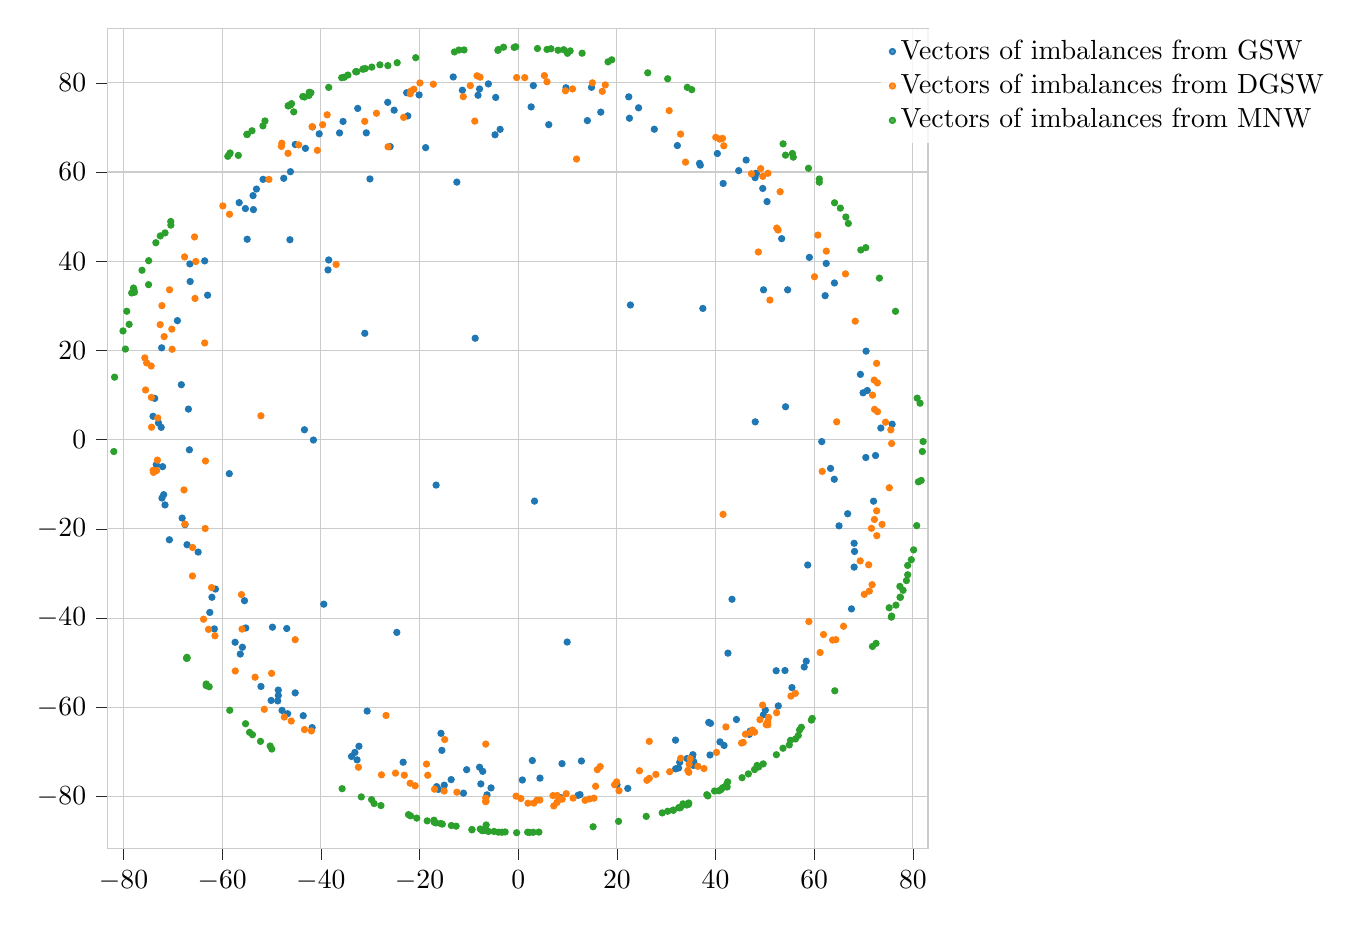
\begin{tikzpicture}

\definecolor{darkorange25512714}{RGB}{255,127,14}
\definecolor{darkslategray38}{RGB}{38,38,38}
\definecolor{forestgreen4416044}{RGB}{44,160,44}
\definecolor{lightgray204}{RGB}{204,204,204}
\definecolor{steelblue31119180}{RGB}{31,119,180}

\begin{axis}[
width=12cm,
height=12cm,
axis line style={lightgray204},
legend cell align={left},
legend style={fill opacity=0.8, draw opacity=1, text opacity=1, at={(1.5,1)}, draw=none},
tick align=outside,
tick pos=left,
x grid style={lightgray204},
xmajorgrids,
xmin=-83.2067624270446, xmax=83.0759530249345,
xtick style={color=darkslategray38},
y grid style={lightgray204},
ymajorgrids,
ymin=-91.6880388118292, ymax=92.2485111427919,
ytick style={color=darkslategray38}
]
\addplot [semithick, steelblue31119180, mark=*, mark size=1, mark options={solid}, only marks]
table {%
32.2584044214495 65.9386568763999
-30.78512025231 68.7889702577337
72.440364565148 -3.56084714298024
-31.08992823135 23.8444022021331
35.5940580599794 -72.2128724567416
58.3909025477593 -49.6674823565428
-72.2037407846078 -13.0958189620082
35.271918282449 -71.2297903844228
-70.699012578559 -22.4460881260352
70.4652216125932 -4.00381322735277
27.5934943162783 69.6029860657221
65.0417469823307 -19.3261587504926
-25.9445743564324 65.7012602015526
38.8841863228764 -70.6977027995228
40.9061831319462 -67.7646673711337
-22.3711169617507 72.5916881875057
-36.2085163933464 68.7732186441355
49.728609698667 33.5941692901107
-49.8110189841752 -42.0433348741018
-32.6558874754734 -71.7918919654906
47.0140395044545 -65.376244693136
-48.6278373077012 -56.1488603780263
70.5220708892224 19.8447876360503
62.4324183640879 39.5100054387699
-46.1585774720407 60.0802314476599
-35.496671284056 71.3509297553594
-43.3250343072014 2.2214075663531
-72.0750252369792 -6.05379458738223
73.5145546414646 2.60061960733761
-15.469635509439 -69.6645520046981
9.92858201556728 -45.3851226072271
-63.5445210013635 40.0852154036615
-51.7117306687373 58.3650565517191
36.7663576635539 61.9446932226637
-8.71521495511577 22.7409185309617
12.1435678304721 -79.7450793566272
-47.8620432214491 -60.7007404143714
40.3750347243597 64.1489314096843
22.4120058248491 76.8646097792012
-25.1440952192131 73.8696031640521
-55.4774723063401 -36.1100611532003
2.62989521214063 74.6121468237154
8.61722999023134 -80.2553914236107
55.4878494652078 -55.5903127999807
-48.6184819841757 -57.3612228608793
36.9147915241226 61.5437715069629
69.914509949494 10.5052875141256
-11.0951599426725 -79.2565652483544
-30.6156024475913 -60.8565302832617
-3.65711718638823 69.5746674390981
63.3174984774895 -6.44555860704591
46.8469333120392 -66.0782918849572
-64.8718044398264 -25.2050458936034
-7.56833618037572 -77.1839710466772
-11.310144915538 78.3473852607746
2.86904121527245 -71.9475349778482
44.695510910438 60.3186013876898
-5.50170588316871 -78.0793195171212
38.6270224756657 -63.3976570441669
75.8031921042529 3.47176771140928
48.0122511931596 58.7478276418118
-4.55826082244179 76.7306598611441
-41.7650338403545 -64.5622905627959
53.409505893534 45.0695346414368
8.88526307026061 -72.6352984043277
-20.0842436314704 77.2946278674008
-48.739557861863 -58.5738919061177
32.5151997855299 -73.6164900702865
12.5336161467112 -79.5892218207455
35.4973356973301 -73.0328014368945
70.7624473395153 11.011416410362
-32.5252717803079 74.2671002390158
-10.4439644224755 -73.998403668327
42.5154700631192 -47.8691247971493
-72.3580516470113 2.76556191728851
41.7334131515087 -68.567040369269
48.050722427563 3.98964067231821
-6.31927292208101 -79.6413727229891
-15.6454859827255 -65.8530219467586
-52.1432394645244 -55.3362868941948
-45.192408960536 66.1849226604328
38.985906930474 -63.6023002403114
-4.69326586973153 68.3523235645167
-55.8997307746974 -46.5433773211604
0.849514366543625 -76.3065008907066
-43.1223552834311 65.3090909826903
-41.7044837624707 70.1181020124392
-74.0158614631308 5.23490266644007
-62.5066619900689 -38.7359985560885
54.197108459558 7.37808465362673
-46.7378168904591 -61.4502786377574
22.2169490391029 -78.1998468213536
67.5611563618523 -37.9437325271889
-7.19194964254755 -74.3726480542728
22.7472306020448 30.1917922504671
68.1846601544919 -25.0638648796997
52.7224603006108 -59.6915580335686
-68.1124833311236 -17.5880196284312
-43.5691012360639 -61.8882003531607
9.68721978321953 78.9026185806715
-62.9540297572674 32.3913549035316
-18.7579787045758 65.4731834425465
20.0302413676354 -77.3671964590653
-13.5855615281493 -76.2214345403727
-69.0742244525684 26.6786143688733
72.0355762419608 -13.7972661302186
-67.5327509300474 -19.0522783873151
-67.1228588819719 -23.5548738064781
-72.9097524679152 3.74287434954817
54.080836277382 -51.7656746726365
69.3668765576836 14.6401594995066
31.9109145158549 -73.8055932753755
54.6218699951625 33.5876366060071
-66.5475315302179 39.40241566771
-68.2761609648053 12.3206924436541
46.2087389936537 62.6854993502268
-66.6428013339522 -2.27611578225907
-57.3759483342749 -45.4321256438847
-47.5172505829085 58.5948273066201
66.7824749745596 -16.6132791464255
-38.5449274390525 38.0546890743992
-71.856018355598 -12.3346633205556
57.9791987046803 -50.9732760619459
61.5350210646747 -0.436132777924667
14.8625614729461 79.0007660917453
-46.9069147680345 -42.3445945471387
-16.181506899167 -78.4131605836978
-39.4047183293266 -36.8883186447915
-62.079009196256 -35.339780932805
-71.5854419791736 -14.6332911579964
-66.4897265970382 35.4564581377113
43.342833219258 -35.7828768319551
-55.2145417893679 -42.2223366512621
-30.0494955875644 58.4569744082907
37.4307325804791 29.4240644199051
-50.0741891133751 -58.473993103024
-6.03830071068439 79.7650747798212
-61.5929339117119 -42.4289545460987
44.2394571824595 -62.7406764068255
-32.2757940906564 -68.7433490573526
-33.7845312277856 -71.0284971743076
-40.3388139928347 68.5642946329428
-72.266582565546 20.5873199674641
-24.5996313535525 -43.2132058432298
-53.0483658673079 56.1874880605418
-14.9821509577675 -77.4682263504023
-58.5565973661462 -7.62276512830875
-66.8389041330287 6.84797938972953
-53.7402545616911 54.7164641076597
-12.4310245384575 57.7434513326038
59.0236570301686 40.8685240561386
50.4446223153189 53.3717984306408
64.099527024871 35.1318418690043
32.7374547673931 -72.3486684735372
3.07510827014208 79.3839490435443
-38.4040307836502 40.2958250145425
-7.83144186364703 78.6300382649299
68.0977007456207 -28.5755211810739
-16.6345637408787 -10.1854716518513
-45.1918547473977 -56.7716551550004
41.5503266464487 57.4350214709958
-61.3567253156031 -33.5013565774428
-41.5033709419344 -0.0849629376979833
35.409695865696 -70.6359754758922
-73.3507634709704 -5.61283228700009
-22.6064612865655 77.7813672044065
31.8966863787351 -67.3724136792563
34.2348354086764 -71.5002136331364
-23.3164788052521 -72.3204791578254
-26.4413144487601 75.6303237862724
14.0247810391753 71.5282771805199
-56.321515260361 -48.0711905268262
62.2225109291443 32.282114560062
52.2926033363182 -51.8150547801773
22.5496147940758 72.0678489342606
-73.6724980883283 9.25582439480754
48.1573099067193 59.7074167018134
50.1005687885256 -60.6353015981225
-46.2663411121317 44.8260452768995
-33.1019141188891 -70.1294637966069
64.0696569961187 -8.87697285071274
-56.5544016901305 53.1436754311971
4.42072127242031 -75.8910310450107
6.19905164153228 70.6269514729997
12.8205115143945 -72.0479931370027
-54.9299979002684 44.9322889061776
49.7056294095111 -61.7056591199924
48.2690935077609 59.6216466570029
-53.6659914487213 51.5796887851568
68.0945920174679 -23.2365582192899
58.6941984750679 -28.1026220069943
-13.1658805954465 81.3210953821928
24.4031648247729 74.3980975889671
-7.82856271221485 -73.4499372459839
3.30903221905349 -13.7852308677481
-16.5266150568404 -77.7979469097883
49.5721093210683 56.3229302952462
-8.13971878634583 77.2139458229984
-55.2909405253252 51.81794402212
16.7432820345378 73.4320509897254
};
\addlegendentry{Vectors of imbalances from GSW}
\addplot [semithick, darkorange25512714, mark=*, mark size=1, mark options={solid}, only marks]
table {%
-6.57300003808273 -68.2611608711121
5.31328927030602 81.6283790119687
-71.764354904977 23.1061308959195
-63.4449039640438 -19.9195951796147
-8.33970209706928 81.5810856990458
-47.9101807910426 66.4691109134433
1.3306360425668 81.171353822595
-62.7735894322806 -42.5364377764579
71.8291420588586 9.98139317644557
61.8898869585487 -43.6865105784712
7.21249723903866 -82.1247637677807
-74.3139818836647 2.79455174815397
-43.3152096732541 -64.9996963741004
75.2276854501355 -10.788391977236
32.9430261449679 -71.4351538792013
19.9517494799329 -76.7281064038012
-47.9979711370703 65.7603383176248
-7.72375358766734 81.2740390108251
-27.711188472057 -75.1495909527575
37.6566222252295 -73.7475013040384
-8.7926184027841 71.4189889184638
72.6955594175556 -21.5271654002011
47.2875546074722 59.617621077416
55.2841557319299 -57.4939438779893
-6.58274032496308 -80.3523689128115
60.7456873960461 45.8617901759081
-75.3165197324567 17.216718113501
-18.5803366136032 -72.7391971670199
-0.421043077751697 -79.9280589745303
-66.0297306902367 -30.5649825808335
72.2345366146534 6.78542359343683
-46.6530675422628 64.1996535494944
60.0634914188462 36.5307859395959
19.5424999298566 -77.3764118273183
30.7078119049722 -74.4468398775456
-63.3884134781183 -4.78155107552455
-52.1459194382976 5.34354297225723
-23.216902282054 72.2580407139287
26.5830481933362 -75.948582008923
64.3969827182105 -44.8482920275507
-28.7210397037759 73.1849081553127
36.4188304027162 -73.242099852905
53.1012894746923 55.5846322390891
9.72805718275821 -79.3823517150815
-40.699251040215 64.8690873864756
46.0770794592862 -66.028882310976
-56.0920735781599 -34.7379747341882
61.6191123852367 -7.11831705077342
72.2076271283572 -17.8935594097667
41.4205859686657 67.5415040179798
-46.0015056181685 -63.0884053114322
17.6619460169287 79.5375825835704
61.2038532603695 -47.7256693729759
50.2753507789513 -63.8940979001035
-63.7760764439446 -40.2584247845739
-51.4678548928031 -60.4561968279941
-73.3006340439803 -6.94216649237462
58.9250225111237 -40.7823741948326
-47.4051195235264 -62.1922959576463
11.8346180209683 62.9157280884327
-74.3533279637824 9.46918678085542
49.0058957476429 -62.7863491657238
-72.569583688022 25.7897082977302
-14.8964229973282 -67.2335424915798
-36.898273563601 39.2833113486128
-75.5233101730811 11.1433872340756
66.3379821833856 37.1733967869614
75.6961200902037 -0.855663772490673
-41.9195823451489 -65.3026016396553
-0.313063649434285 81.1890994125047
52.3827214982965 -61.2169024394471
-58.5106022455496 50.5310991902242
-17.1980055153357 79.6901844251516
74.4626558925317 3.90962509646072
-21.7366262033914 78.1685181778511
34.3881107362911 -74.1794393887005
-59.8567668074318 52.4035276098963
51.021635059922 31.2934497951315
-72.2105258327193 30.0434719454017
-73.9947183137871 -6.87707390302968
50.5833362841406 -63.2342888641987
40.8602617010832 67.382366964869
-38.7197732847345 72.8345266265523
-16.954667480472 -78.3699687247616
-73.923973086827 -7.33905734184872
-67.7421788494786 -11.2682498321696
-49.9830050847466 -52.3968606951822
71.1774070923227 -33.9552330960755
-15.0099760098353 -78.7707975887178
65.9468289478493 -41.8467472661402
3.81195050861152 -80.8322200839502
33.9203784737362 62.226702687568
32.9206691667439 68.512121918567
52.4129614814392 47.4314990433144
40.0500943358723 67.7793933447627
-75.6792169406868 18.3315409155097
47.0949450897698 -65.655360511689
-73.1284594732511 -4.58900249557341
-32.3882612426196 -73.4438222093753
-70.2068878964051 24.7797250499416
56.1802781596985 -56.8856664042302
50.7518339126723 -62.2824305654851
-55.9746396122132 -42.4743244734344
-21.887559145259 77.5412237983377
71.7409962597615 -32.5184588161948
42.1092828388692 -64.4087617587658
41.5316446153193 -16.7504781530775
48.6831535137112 42.0716193908679
-26.3749714172762 65.6590299810163
-67.6199481225327 40.9797545425837
15.6988994752527 -77.7137583741195
15.3589943744872 -80.3911288201285
70.1548389217906 -34.6786292149383
72.8366458199767 6.26979190842479
50.6215690734576 59.7221656184365
8.22525679937225 -80.7724163313869
72.8207966405374 12.7269079974426
-21.1434831835054 78.5618381464854
-9.70837918060963 79.3804590860885
-6.60926846617041 -81.1571064837996
24.5893168574033 -74.2429415588415
62.4516183678715 42.2693896922943
20.4422566121218 -78.7043640262414
14.4367007422784 -80.5604606592273
72.6649637606492 -15.9591100495488
34.5841492174828 -74.5763020266891
-63.5462465243349 21.6818421277734
47.4971644940791 -65.1061947166628
27.9107679083036 -75.0578091364408
16.6251976328391 -73.3028640258055
45.2804507776418 -68.01071383502
-41.7655467255293 70.1589189138736
7.85134253805627 -81.3566798147062
-74.3882078494514 16.5159830225486
30.6076420354553 73.7720387278967
45.6169097978524 -67.8922297911005
75.5386169560949 2.19494710819997
-18.3329399939065 -75.2504775398938
52.6816586996245 47.0076687033763
-62.1456745635549 -33.1685952753351
-65.3446064858711 39.9436891474197
16.0414766261006 -73.9862045559487
47.9277978675119 -65.5817819912364
64.5613458536562 3.99092816219679
-65.9956091469268 -24.1757734179857
-39.6343408296442 70.6160439478426
73.7607409974621 -18.9948589641752
71.6136020356969 -19.8846487073678
11.1325222087021 -80.3659572563612
-61.4642427781268 -43.9639579740379
-21.8954907230776 -77.034649851516
26.0911664307507 -76.3752101954848
4.38907194027385 -80.8097514704446
-70.1468409669891 20.2668363372205
-65.5087742368552 31.6658549539105
11.0210635208653 78.6301103204124
-65.5961249796429 45.4535994795794
69.3291910409258 -27.1810131660296
-24.8659481292113 -74.7702004638136
71.041901089032 -28.0609331311978
-45.1973778751478 -44.8466445126558
13.5624378474542 -80.8644813434682
49.5400014350438 -59.5193081179167
40.1998641919371 -70.1229246785335
17.0433444172601 78.0923551620482
-70.6669754806265 33.5997661723637
-44.4978134670329 66.0870028806813
7.05896022958024 -79.8073269067423
-6.51743134451127 -81.0819837991814
-11.1281852549619 76.906086649774
-19.9161240534128 79.9781603061949
3.16276480584934 -81.4822986322097
68.3190041403423 26.5673395410284
34.655935680701 -72.7811297312628
5.8409670183604 80.2398587689081
7.9132141238474 -79.7940079316188
-23.0827154829219 -75.233814862388
1.97867090842553 -81.5034600315662
41.6784704848857 65.8819126647018
-73.0557418654925 4.86799477330016
-57.3441217583035 -51.8583295955288
72.6537922207366 17.1091737642045
15.0352302057771 80.0025909197412
-67.5353241366693 -18.9287325023133
-50.5287383970326 58.348583495255
9.5878300302957 78.218543784947
49.154483598965 60.7613447689411
-20.8765323801118 -77.604648380287
-53.3285637981133 -53.2636074977827
34.8615228034461 -71.5457564737417
-31.1025470949625 71.3638997387965
-26.7835187468224 -61.8410963111955
0.543045751687271 -80.4661432444305
50.6085027768425 -63.9376431718791
72.1715286361006 13.3412486785492
26.5738162950215 -67.6500155330411
-12.4203949680781 -79.0385212378065
49.5892921540261 59.0394212886869
8.9247478527499 -80.58936760015
63.7352328464401 -44.9312747228185
};
\addlegendentry{Vectors of imbalances from DGSW}
\addplot [semithick, forestgreen4416044, mark=*, mark size=1, mark options={solid}, only marks]
table {%
42.2187897858552 -77.3466940442597
78.0231469121335 -33.772395713265
-46.1442669587632 75.0371565746242
69.4476477767307 42.5379254629481
75.1985563375172 -37.6919428587142
-58.3944088406366 64.2769693161983
-7.68638983131354 -87.2883326391492
54.1862309073416 63.7864337255736
-77.7839402022082 33.0503299527512
-12.925007837351 86.9311981623245
-29.6674529170566 83.5328546793324
55.1979254371374 -67.422152465925
65.3080465569369 51.9129513511809
72.5392154462576 -45.6807350341835
-6.48706046095136 -86.3902228239314
-77.9651249025985 33.9935379895219
66.4216824401156 49.9172400231736
-35.7717401312479 81.1592396977042
-3.96406001327461 -88.0084588083677
77.4719971529889 -35.3514852954127
-26.4141920953607 83.8643174162537
48.4301433711403 -73.0356596455354
73.2179300323774 36.2155066766447
-18.44172561986 -85.4690506005778
38.2383618773534 -79.6025673165431
-43.6563871602343 76.9311917968408
12.9579814274716 86.6469198194951
53.6738519633173 -69.1848704004217
-6.86641748124642 -87.6064846195727
-67.1502619090359 -48.8091392879473
25.952205897638 -84.4631909556707
-29.2009909275812 -81.5862073696289
-15.3737235345191 -86.1973798979606
33.415118942956 -81.6568512232002
32.5171405054778 -82.5253907566525
-63.2433479268035 -55.1346343086845
-13.5397525775156 -86.5181613868655
9.99297555677269 86.6187920639674
42.3524908328557 -77.8854860996471
-12.0252739229913 87.3476584597596
18.2103512130162 84.7059395816794
-58.4632973873028 -60.6773029461017
-31.7964522243784 -80.100454634
41.440750669627 -78.0446410923118
78.9541008921074 -30.2920824170314
-0.816888685038943 87.9570067527856
-81.962246186164 -2.66259885460674
48.7456601630974 -73.3852275414089
-54.9535122673688 68.4397524995277
-0.314465846938702 -88.1275241790371
47.9097974854561 -73.9739700930215
-4.89811627385143 -87.8421250721293
29.1934517062559 -83.684335714213
38.4484231358075 -79.8706781766431
59.4310823465951 -62.8796657551419
77.3684818331768 -32.8951184903521
81.6894907532241 -9.14961034195322
-46.6343752078538 74.8300614505986
-73.441099435793 44.155592018068
-42.4045381742229 77.1735003823969
-38.4022279832157 78.9804095118892
-32.9014616767014 82.5024630187932
45.3823545893373 -75.79534019663
-42.015135967352 77.7885277389825
-24.5269357281049 84.511665204645
-17.0038656648721 -85.7987104521118
-67.2212395286512 -49.0403389592042
-29.714228116071 -80.7144225955582
-12.5770188711524 -86.660932938304
-30.9837920304525 83.1987122988655
4.19895235057013 -87.9912690078653
-45.4905720895866 73.4933642416459
-54.9535122673688 68.4397524995277
-31.4424170452379 83.080593053039
-80.0991007782733 24.3774013116847
3.90657479153912 87.6984715536424
9.23359831546317 87.4350928315283
55.5784916184793 64.1616937597938
30.3004919117379 80.9193361225195
-67.0911982352291 -48.9813144653981
-32.9014616767014 82.5024630187932
-54.9535122673688 68.4397524995277
-74.8991285539727 40.1298330980038
42.46385870097 -76.728702545093
78.7022989975578 -31.6002334077482
-31.4424170452379 83.080593053039
-72.5392154462576 45.6807350341835
82.081670601679 -0.424379279241261
-58.8581799496873 63.5287269634791
-4.10727910061256 87.286775600175
10.5310794892521 87.165930242223
-71.5823554952609 46.3548868304919
-22.2351490492534 -84.0696733443516
26.2651293500311 82.2466230933601
58.845015371017 60.8536243618627
80.7813402406485 -19.2799570546429
-50.2725293502983 -68.6895460786956
57.39917924558 -64.4901424303505
-15.7142724725679 -86.0671374615144
-2.96260617632121 87.996348634828
-52.2339566837629 -67.6454324913073
-70.3995840955867 48.1054770938384
49.6661696654906 -72.6974908480675
-28.0291168826783 84.0403418551762
8.08644853861669 87.3085708250168
-21.8257744264935 -84.3408887965517
81.4581303655903 8.17269930820277
-76.2506327791724 37.9768241026871
61.0371406200021 57.7266233929456
20.3463197825398 -85.5787298826736
-35.2624922596778 81.2656100798938
-3.26677630779439 -88.0201786102107
-74.9216103186033 34.7551046023069
53.6997208412113 66.3226738837107
77.4152171453639 -35.329131935907
76.4835647879187 28.7761505072825
-78.3428589370765 32.8968731618872
34.5686869483397 -81.4639775620498
34.5142388198075 -81.7433300218808
-43.3190322947306 76.8342334361762
6.64825965678075 87.6452302822057
-4.00818660309855 87.4801723539888
79.6873211276208 -26.9212330641394
76.5703448041154 -37.1013015513093
32.6999183566784 -82.4965027288624
40.6687172716727 -78.7268494600129
-27.8191683831229 -82.0402572335621
-7.29555819197313 -87.6637845266095
31.4424170452379 -83.080593053039
-9.37443947523563 -87.445908099336
80.8769271823698 9.30640216988008
70.4639975898609 43.0472785477075
-10.9801316187731 87.3793587235945
-35.6893969632735 -78.2513306014348
-79.3390393412207 28.7896107794872
52.3354781922899 -70.6375628327244
41.0949895214153 -78.4695764238237
-46.5302369248153 74.9158533694372
81.1227558728864 -9.45599113924786
-81.8074713904174 14.0147310400486
-51.3311920558631 71.459679452643
-70.4231503194558 48.9129041925724
2.29937861974223 -88.0664238332306
61.0357745160335 58.4421520977969
-63.225046115407 -54.7775440797247
-34.5142388198075 81.7433300218808
-53.9492261309421 69.2618691194463
-42.3524908328557 77.8854860996471
-16.6891348918289 -85.9292208968939
-77.8739093057425 33.5568700747098
-17.080050287812 -85.3224087644127
64.1808437260021 -56.3128138625946
39.795916694841 -78.7730116467664
-53.8606974942242 -66.1543370764642
-20.7739110886551 85.643028796324
18.9631395114811 85.1616663001613
-9.37443947523563 -87.445908099336
-51.7351907591295 70.3541372101725
5.85122805188153 87.4916426484024
-2.64184064075553 -87.9596973653116
-54.4464551680128 -65.6204430482631
46.6577768669396 -74.939248839053
56.2165314509822 -67.1045055940129
-20.5626001914468 -84.8518475173801
34.5142388198075 -81.7433300218808
30.3023194240771 -83.3183047780515
32.6999183566784 -82.4965027288624
-49.944772187605 -69.3668746315776
34.1589629881419 -81.9183726946166
54.9535122673688 -68.4397524995277
59.6023312384644 -62.5014859069912
66.9239989515675 48.4756740505335
-56.7250914543114 63.7318291442794
35.1853402117036 78.4735300110768
64.128029922626 53.1064712474145
-45.9435368464641 75.3453762712079
34.2813998247644 78.9928361589285
-6.66694287554573 -87.5876813976652
-55.2606922057658 -63.6904883792454
56.7833188335 -66.3200011365378
75.6363254119942 -39.7897714255417
3.04039358458121 -88.0311217021388
1.91998541247223 -88.0074535417625
15.1858334477982 -86.7936129072831
-0.488524847611382 88.0884000921092
80.1568253342377 -24.7185706093779
-78.859250043601 25.8521209307207
-62.6325630587417 -55.4056754966273
78.9419470733631 -28.2006883099576
71.806409466616 -46.3726100483838
31.4424170452379 -83.080593053039
-6.02425807777213 -87.8481312656348
-58.4753203369045 64.0726217004867
55.7586695741879 63.3430049946929
57.0319682031286 -65.090020035929
32.9014616767014 -82.5024630187932
81.9266774423736 -2.65104999273622
75.6994830200278 -39.5559136848349
-32.6999183566784 82.4965027288624
-79.614193821701 20.3088491574854
};
\addlegendentry{Vectors of imbalances from MNW}
\end{axis}

\end{tikzpicture}

\caption{Results of experiment 1 from section \ref{exp1_A_T}. Vectors of imbalances using the modified GSW and DGSW where the update direction is computed by multiplying the pivot vector by $\textbf{B}^T$, as well as from the maximizing naive walk.}
\label{A_T_instead_of_lstsq}
\end{figure}
The plot of the outputs from experiment 1 are shown in figure \ref{A_T_instead_of_lstsq}. We can see that this modification seems like it now minimizes output balance by pushing the vector of imbalances away from \textbf{0}, which was surprising to us at least. This seems like it could be useful to sample from unbalanced group assignments, or to find a subset to remove to maximize along one dimension for example. This might be equivalent to an already known algorithm, but if not I think there might be interesting applications to this, as pseudoboolean maximization of positive definite quadratic forms is an NP problem as can be seen in \cite{gritzmann19890}. 

For this exact distribution of input vectors we can see that the maximizing naive walk is always a step further from \textbf{0}, as if there was a limit that this GSW variant could not go over. It would be interesting to understand why that is, and whether that could be used to sample on the outer part of a zonotope for example. We can notice as well that the DGSW vectors of imbalances seem to be more often on the circle than the GSW vectors of imbalances which sometimes ended up in the middle.

\begin{figure}[h!]
\centering
% This file was created with tikzplotlib v0.10.1.
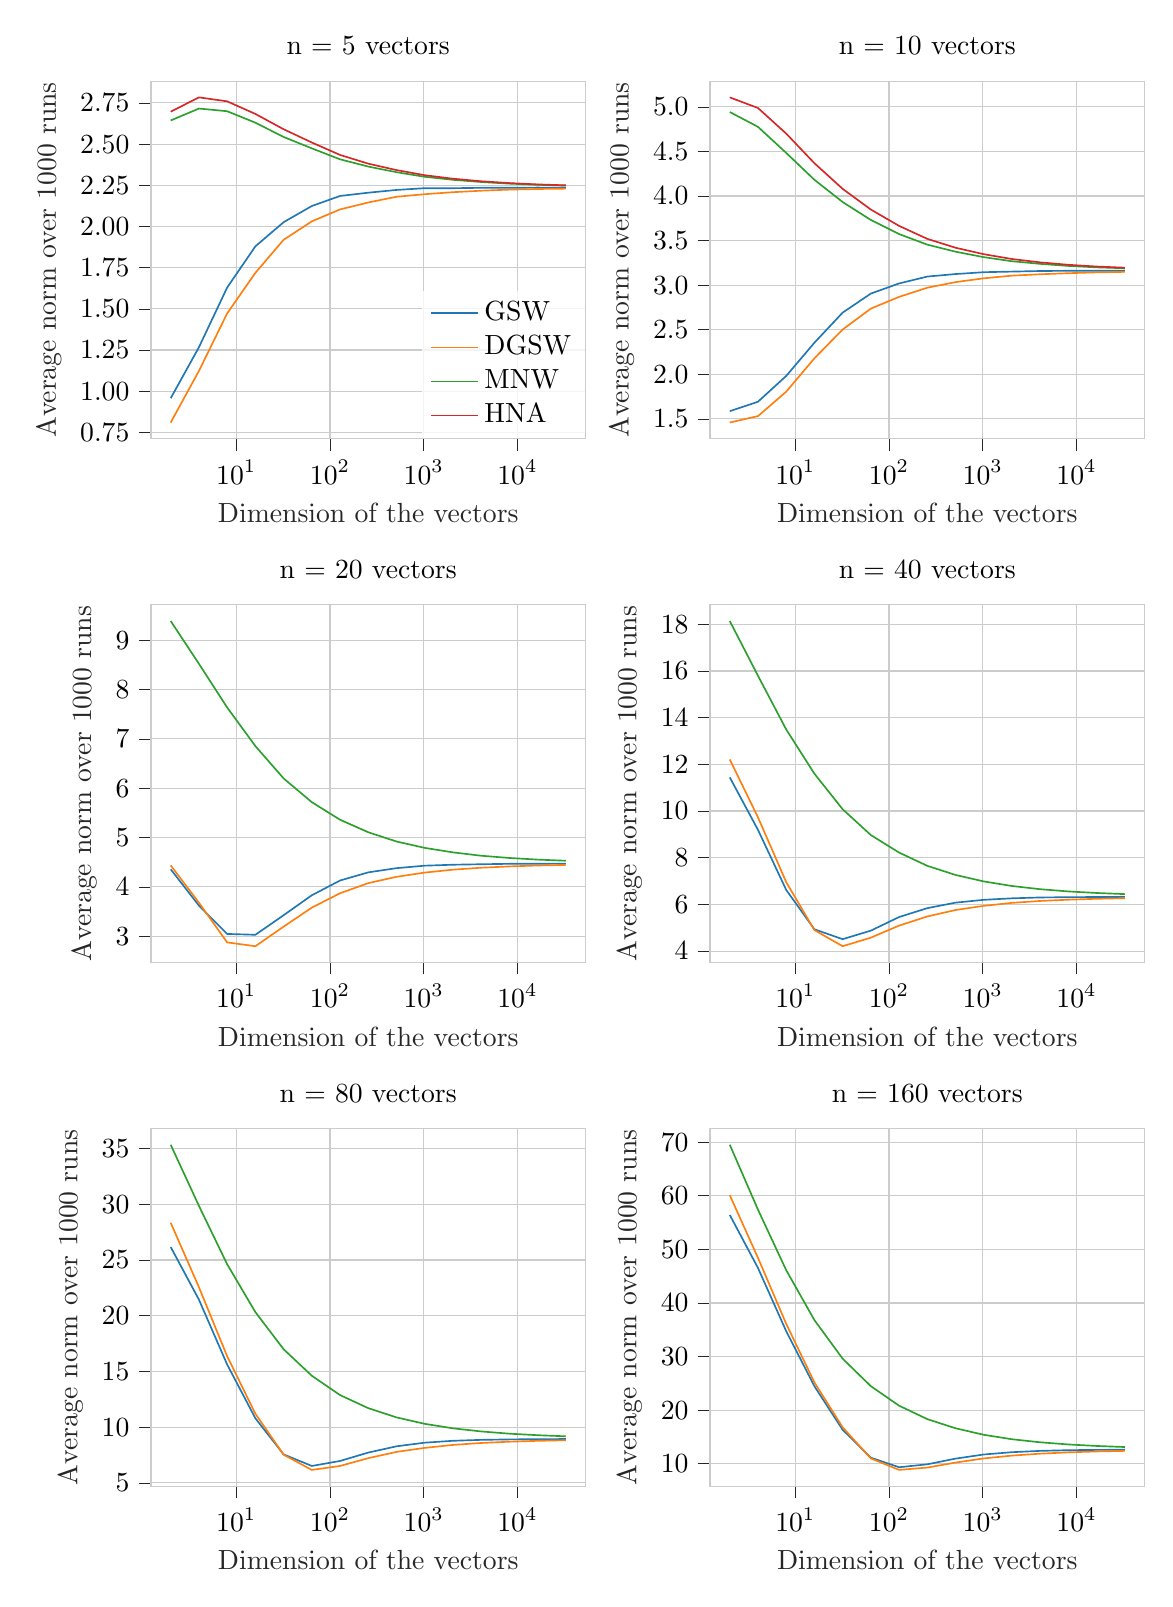
\begin{tikzpicture}

\definecolor{crimson2143940}{RGB}{214,39,40}
\definecolor{darkorange25512714}{RGB}{255,127,14}
\definecolor{darkslategray38}{RGB}{38,38,38}
\definecolor{forestgreen4416044}{RGB}{44,160,44}
\definecolor{lightgray204}{RGB}{204,204,204}
\definecolor{steelblue31119180}{RGB}{31,119,180}

\begin{groupplot}[group style={group size=2 by 3, vertical sep=60 pt, horizontal sep=45 pt,ylabels at=edge left},width=7.1cm]
\nextgroupplot[
axis line style={lightgray204},
legend cell align={left},
legend style={fill opacity=0.8, draw opacity=1, text opacity=1, draw=none,anchor=south east,at={(1,0)}},
log basis x={10},
tick align=outside,
tick pos=left,
title={n = 5 vectors},
x grid style={lightgray204},
xlabel=\textcolor{darkslategray38}{Dimension of the vectors},
xmajorgrids,
xmin=1.23114441334492, xmax=53231.7730476022,
xmode=log,
xtick style={color=darkslategray38},
xtick={0.1,1,10,100,1000,10000,100000,1000000},
xticklabels={
  \(\displaystyle 10^{-1}\),
  \(\displaystyle 10^{0}\),
  \(\displaystyle 10^{1}\),
  \(\displaystyle 10^{2}\),
  \(\displaystyle 10^{3}\),
  \(\displaystyle 10^{4}\),
  \(\displaystyle 10^{5}\),
  \(\displaystyle 10^{6}\)
},
y grid style={lightgray204},
ylabel=\textcolor{darkslategray38}{Average norm over 1000 runs},
ymajorgrids,
ymin=0.711103890240406, ymax=2.88251918763148,
ytick style={color=darkslategray38},
ytick={0.5,0.75,1,1.25,1.5,1.75,2,2.25,2.5,2.75,3},
yticklabels={
  \(\displaystyle 0.50\),
  \(\displaystyle 0.75\),
  \(\displaystyle 1.00\),
  \(\displaystyle 1.25\),
  \(\displaystyle 1.50\),
  \(\displaystyle 1.75\),
  \(\displaystyle 2.00\),
  \(\displaystyle 2.25\),
  \(\displaystyle 2.50\),
  \(\displaystyle 2.75\),
  \(\displaystyle 3.00\)
}
]
\addplot [semithick, steelblue31119180]
table {%
2 0.957286687057037
4 1.26693103742326
8 1.62925617377438
16 1.87934820112141
32 2.02583317845528
64 2.12412788063995
128 2.18518392602633
256 2.20505391197423
512 2.22176942944221
1024 2.23237575733488
2048 2.23231027925824
4096 2.2346968632166
8192 2.2346724462055
16384 2.23616819929773
32768 2.2353426161487
};
\addlegendentry{GSW}
\addplot [semithick, darkorange25512714]
table {%
2 0.809804585576364
4 1.12304343831528
8 1.47207913881439
16 1.7184766030907
32 1.919029888876
64 2.03095060188598
128 2.10352567374982
256 2.14562760424858
512 2.18034157421254
1024 2.19593020812204
2048 2.20812169748943
4096 2.21715155481619
8192 2.22366059716972
16384 2.22751804938534
32768 2.2296345046542
};
\addlegendentry{DGSW}
\addplot [semithick, forestgreen4416044]
table {%
2 2.64359718855282
4 2.71595797039376
8 2.69971797837721
16 2.63012691815886
32 2.54356088000909
64 2.47438705773972
128 2.40773109636108
256 2.3637690079093
512 2.32952634734498
1024 2.30164497892981
2048 2.28335852608421
4096 2.26992342256507
8192 2.25999213652007
16384 2.25305051607927
32768 2.24819113694204
};
\addlegendentry{MNW}
\addplot [semithick, crimson2143940]
table {%
2 2.6968191561342
4 2.78381849229553
8 2.75967342809227
16 2.68322283348924
32 2.59038232360164
64 2.50977247167432
128 2.43434792587064
256 2.38132690870505
512 2.34239753303156
1024 2.31124300213559
2048 2.28998313509474
4096 2.27444492523562
8192 2.26350200287688
16384 2.25538963383513
32768 2.2498497186997
};
\addlegendentry{HNA}

\nextgroupplot[
axis line style={lightgray204},
log basis x={10},
tick align=outside,
tick pos=left,
title={n = 10 vectors},
x grid style={lightgray204},
xlabel=\textcolor{darkslategray38}{Dimension of the vectors},
xmajorgrids,
xmin=1.23114441334492, xmax=53231.7730476022,
xmode=log,
xtick style={color=darkslategray38},
xtick={0.1,1,10,100,1000,10000,100000,1000000},
xticklabels={
  \(\displaystyle 10^{-1}\),
  \(\displaystyle 10^{0}\),
  \(\displaystyle 10^{1}\),
  \(\displaystyle 10^{2}\),
  \(\displaystyle 10^{3}\),
  \(\displaystyle 10^{4}\),
  \(\displaystyle 10^{5}\),
  \(\displaystyle 10^{6}\)
},
y grid style={lightgray204},
ylabel=\textcolor{darkslategray38}{Average norm over 1000 runs},
ymajorgrids,
ymin=1.27601532645222, ymax=5.28875986022178,
ytick style={color=darkslategray38},
ytick={1,1.5,2,2.5,3,3.5,4,4.5,5,5.5},
yticklabels={
  \(\displaystyle 1.0\),
  \(\displaystyle 1.5\),
  \(\displaystyle 2.0\),
  \(\displaystyle 2.5\),
  \(\displaystyle 3.0\),
  \(\displaystyle 3.5\),
  \(\displaystyle 4.0\),
  \(\displaystyle 4.5\),
  \(\displaystyle 5.0\),
  \(\displaystyle 5.5\)
}
]
\addplot [semithick, steelblue31119180]
table {%
2 1.58615087944013
4 1.69175299717534
8 1.98077933892884
16 2.35404043335654
32 2.69120670236179
64 2.90511767752765
128 3.01860366843285
256 3.09590132775362
512 3.12398158300726
1024 3.14488645717609
2048 3.15159495409433
4096 3.15813939880135
8192 3.1606237802959
16384 3.16106337103759
32768 3.16166000630415
};
\addplot [semithick, darkorange25512714]
table {%
2 1.45841280525992
4 1.53019675189929
8 1.80445781069704
16 2.17866892163164
32 2.5018618100923
64 2.73641616641356
128 2.86792051867417
256 2.97065514286614
512 3.03345228888961
1024 3.07626732293833
2048 3.10617944646771
4096 3.12158140264402
8192 3.13357673910568
16384 3.14304498652317
32768 3.14862699261037
};
\addplot [semithick, forestgreen4416044]
table {%
2 4.94214825127017
4 4.77551741535279
8 4.48314093066987
16 4.18132154616482
32 3.93200700278754
64 3.73069615705922
128 3.57263076829111
256 3.45399182129845
512 3.37496748563767
1024 3.31373663423724
2048 3.26783387666002
4096 3.23837298892978
8192 3.21530063202238
16384 3.19906330139869
32768 3.18925708954316
};
\addplot [semithick, crimson2143940]
table {%
2 5.10636238141407
4 4.9868157521721
8 4.69986041555852
16 4.36739203459516
32 4.07994606567094
64 3.84758460894373
128 3.66447022258189
256 3.51888799215734
512 3.41938120338708
1024 3.34690888999215
2048 3.29271965155926
4096 3.2550985339455
8192 3.22782349058548
16384 3.20838763136517
32768 3.19550084856252
};

\nextgroupplot[
axis line style={lightgray204},
log basis x={10},
tick align=outside,
tick pos=left,
title={n = 20 vectors},
x grid style={lightgray204},
xlabel=\textcolor{darkslategray38}{Dimension of the vectors},
xmajorgrids,
xmin=1.23114441334492, xmax=53231.7730476022,
xmode=log,
xtick style={color=darkslategray38},
xtick={0.1,1,10,100,1000,10000,100000,1000000},
xticklabels={
  \(\displaystyle 10^{-1}\),
  \(\displaystyle 10^{0}\),
  \(\displaystyle 10^{1}\),
  \(\displaystyle 10^{2}\),
  \(\displaystyle 10^{3}\),
  \(\displaystyle 10^{4}\),
  \(\displaystyle 10^{5}\),
  \(\displaystyle 10^{6}\)
},
y grid style={lightgray204},
ylabel=\textcolor{darkslategray38}{Average norm over 1000 runs},
ymajorgrids,
ymin=2.46511533756539, ymax=9.71985486308159,
ytick style={color=darkslategray38},
ytick={2,3,4,5,6,7,8,9,10},
yticklabels={
  \(\displaystyle 2\),
  \(\displaystyle 3\),
  \(\displaystyle 4\),
  \(\displaystyle 5\),
  \(\displaystyle 6\),
  \(\displaystyle 7\),
  \(\displaystyle 8\),
  \(\displaystyle 9\),
  \(\displaystyle 10\)
}
]
\addplot [semithick, steelblue31119180]
table {%
2 4.35445280728497
4 3.61851467161566
8 3.04413542819236
16 3.02668545113243
32 3.42325807771876
64 3.82817920299293
128 4.12731902130168
256 4.29273550532562
512 4.37821589187115
1024 4.42841907178844
2048 4.44776299531833
4096 4.45753682583283
8192 4.4661180537183
16384 4.46814187481386
32768 4.47057922719581
};
\addplot [semithick, darkorange25512714]
table {%
2 4.43359514866721
4 3.67704533440202
8 2.87235313988013
16 2.79487622508885
32 3.19197429522228
64 3.57706450122827
128 3.86938591219876
256 4.07405678656348
512 4.20274642125186
1024 4.2882242748087
2048 4.34726511455866
4096 4.38718268165739
8192 4.41304629329981
16384 4.43188730520729
32768 4.44433428225971
};
\addplot [semithick, forestgreen4416044]
table {%
2 9.39009397555812
4 8.52349887806927
8 7.6370197187959
16 6.85466277251213
32 6.19860165973379
64 5.71678251925272
128 5.36054803599954
256 5.10631216365618
512 4.91903832579138
1024 4.78971883594271
2048 4.69859667601255
4096 4.630334862098
8192 4.58500243503901
16384 4.55175862266575
32768 4.52848873868708
};

\nextgroupplot[
axis line style={lightgray204},
log basis x={10},
tick align=outside,
tick pos=left,
title={n = 40 vectors},
x grid style={lightgray204},
xlabel=\textcolor{darkslategray38}{Dimension of the vectors},
xmajorgrids,
xmin=1.23114441334492, xmax=53231.7730476022,
xmode=log,
xtick style={color=darkslategray38},
xtick={0.1,1,10,100,1000,10000,100000,1000000},
xticklabels={
  \(\displaystyle 10^{-1}\),
  \(\displaystyle 10^{0}\),
  \(\displaystyle 10^{1}\),
  \(\displaystyle 10^{2}\),
  \(\displaystyle 10^{3}\),
  \(\displaystyle 10^{4}\),
  \(\displaystyle 10^{5}\),
  \(\displaystyle 10^{6}\)
},
y grid style={lightgray204},
ylabel=\textcolor{darkslategray38}{Average norm over 1000 runs},
ymajorgrids,
ymin=3.51099570470091, ymax=18.8373349350054,
ytick style={color=darkslategray38},
ytick={2,4,6,8,10,12,14,16,18,20},
yticklabels={
  \(\displaystyle 2\),
  \(\displaystyle 4\),
  \(\displaystyle 6\),
  \(\displaystyle 8\),
  \(\displaystyle 10\),
  \(\displaystyle 12\),
  \(\displaystyle 14\),
  \(\displaystyle 16\),
  \(\displaystyle 18\),
  \(\displaystyle 20\)
}
]
\addplot [semithick, steelblue31119180]
table {%
2 11.4413696168594
4 9.19196106644453
8 6.62041051621656
16 4.93187487358655
32 4.50865018206496
64 4.87519300758341
128 5.45732907478117
256 5.83893415803102
512 6.07398880175621
1024 6.19533875155021
2048 6.25984711913787
4096 6.29665757639744
8192 6.30744534358293
16384 6.31640431728546
32768 6.32001847756238
};
\addplot [semithick, darkorange25512714]
table {%
2 12.2100215579241
4 9.72881324327746
8 6.95187916520608
16 4.89789679815998
32 4.20764748789657
64 4.57451192981306
128 5.0906616505781
256 5.48279690370295
512 5.7586260279104
1024 5.93771119136038
2048 6.06495245732353
4096 6.14722468958825
8192 6.20014884909289
16384 6.24029525597681
32768 6.26476307382385
};
\addplot [semithick, forestgreen4416044]
table {%
2 18.1406831518098
4 15.7954196114078
8 13.4951754877111
16 11.5984935217289
32 10.0770143069862
64 8.9692305701984
128 8.22000777088385
256 7.65200952777181
512 7.26147098309957
1024 6.98424926845207
2048 6.78754307957096
4096 6.650806505357
8192 6.55468625288236
16384 6.48873909860577
32768 6.4400005824825
};

\nextgroupplot[
axis line style={lightgray204},
log basis x={10},
tick align=outside,
tick pos=left,
title={n = 80 vectors},
x grid style={lightgray204},
xlabel=\textcolor{darkslategray38}{Dimension of the vectors},
xmajorgrids,
xmin=1.23114441334492, xmax=53231.7730476022,
xmode=log,
xtick style={color=darkslategray38},
xtick={0.1,1,10,100,1000,10000,100000,1000000},
xticklabels={
  \(\displaystyle 10^{-1}\),
  \(\displaystyle 10^{0}\),
  \(\displaystyle 10^{1}\),
  \(\displaystyle 10^{2}\),
  \(\displaystyle 10^{3}\),
  \(\displaystyle 10^{4}\),
  \(\displaystyle 10^{5}\),
  \(\displaystyle 10^{6}\)
},
y grid style={lightgray204},
ylabel=\textcolor{darkslategray38}{Average norm over 1000 runs},
ymajorgrids,
ymin=4.70333599113201, ymax=36.7942840182604,
ytick style={color=darkslategray38},
ytick={0,5,10,15,20,25,30,35,40},
yticklabels={
  \(\displaystyle 0\),
  \(\displaystyle 5\),
  \(\displaystyle 10\),
  \(\displaystyle 15\),
  \(\displaystyle 20\),
  \(\displaystyle 25\),
  \(\displaystyle 30\),
  \(\displaystyle 35\),
  \(\displaystyle 40\)
}
]
\addplot [semithick, steelblue31119180]
table {%
2 26.155709985768
4 21.4398954767142
8 15.6188619528764
16 10.7939605608373
32 7.5570127010587
64 6.51739464548474
128 6.96360346870058
256 7.71727532224011
512 8.28040753607601
1024 8.6056407677305
2048 8.77505113437528
4096 8.85830014113856
8192 8.89895413437589
16384 8.92032629159847
32768 8.93145982900229
};
\addplot [semithick, darkorange25512714]
table {%
2 28.3343575908632
4 22.5525426112266
8 16.3647169038532
16 11.2030177444302
32 7.52803460753208
64 6.16201544691057
128 6.5165409265363
256 7.21509842642689
512 7.77943665030694
1024 8.13884688563795
2048 8.40400033733163
4096 8.57833077470634
8192 8.69331848794077
16384 8.77125193173225
32768 8.82398712526377
};
\addplot [semithick, forestgreen4416044]
table {%
2 35.3356045624818
4 29.8524311298087
8 24.6167252274202
16 20.3196935858281
32 16.9933381405461
64 14.6110445521679
128 12.8773039736156
256 11.7050306376698
512 10.8757512124917
1024 10.2971313470562
2048 9.89487419606316
4096 9.61323064527042
8192 9.41434716475834
16384 9.27685063873229
32768 9.17851361821804
};

\nextgroupplot[
axis line style={lightgray204},
log basis x={10},
tick align=outside,
tick pos=left,
title={n = 160 vectors},
x grid style={lightgray204},
xlabel=\textcolor{darkslategray38}{Dimension of the vectors},
xmajorgrids,
xmin=1.23114441334492, xmax=53231.7730476022,
xmode=log,
xtick style={color=darkslategray38},
xtick={0.1,1,10,100,1000,10000,100000,1000000},
xticklabels={
  \(\displaystyle 10^{-1}\),
  \(\displaystyle 10^{0}\),
  \(\displaystyle 10^{1}\),
  \(\displaystyle 10^{2}\),
  \(\displaystyle 10^{3}\),
  \(\displaystyle 10^{4}\),
  \(\displaystyle 10^{5}\),
  \(\displaystyle 10^{6}\)
},
y grid style={lightgray204},
ylabel=\textcolor{darkslategray38}{Average norm over 1000 runs},
ymajorgrids,
ymin=5.81953179559757, ymax=72.5460331431545,
ytick style={color=darkslategray38},
ytick={0,10,20,30,40,50,60,70,80},
yticklabels={
  \(\displaystyle 0\),
  \(\displaystyle 10\),
  \(\displaystyle 20\),
  \(\displaystyle 30\),
  \(\displaystyle 40\),
  \(\displaystyle 50\),
  \(\displaystyle 60\),
  \(\displaystyle 70\),
  \(\displaystyle 80\)
}
]
\addplot [semithick, steelblue31119180]
table {%
2 56.4157695359282
4 46.5201925639667
8 34.725385417671
16 24.4611270278844
32 16.3412413319146
64 11.1342333543456
128 9.34869123242952
256 9.89686320497877
512 10.9546177596886
1024 11.7263043058913
2048 12.1563570971504
4096 12.4029657726301
8192 12.5306827141335
16384 12.5849153172608
32768 12.6175730046919
};
\addplot [semithick, darkorange25512714]
table {%
2 60.1005073882231
4 48.4121611633676
8 36.093682274419
16 25.1658753248385
32 16.7990456093371
64 10.9889010399708
128 8.85255458412289
256 9.29168313063863
512 10.2167038450993
1024 10.9962827667789
2048 11.5202771785862
4096 11.8801860200103
8192 12.1300161795572
16384 12.2923867782903
32768 12.4019008278777
};
\addplot [semithick, forestgreen4416044]
table {%
2 69.5130103546292
4 57.3996771863378
8 46.1102377610629
16 36.7958168680131
32 29.6027748888002
64 24.4696162836931
128 20.834857100957
256 18.3259147096778
512 16.6213980146746
1024 15.403221289702
2048 14.5718168590642
4096 14.0038385238994
8192 13.6002160191167
16384 13.3192137731733
32768 13.1201249958734
};
\end{groupplot}

\end{tikzpicture}

\caption{Results of experiment 2 (section \ref{exp2_A_T}): comparing the modified GSW and DGSW with norm of the vector of imbalances maximizing algorithms.}
\label{A_T_instead_of_lstsq_2}
\end{figure}
Results of experiment \ref{exp2_A_T} are available in figure \ref{A_T_instead_of_lstsq_2}. We can see that for small $n$, using $\textbf{B}^T$ doesn't actually maximize the norm for small dimensions even though it seems to asymptotically do so when the dimension grows. For bigger $n$'s though, this variant seems to be decent at maximizing the norm of the vector of imbalances, even though it is worse at it than the naive walk for this particular distribution of input vectors. It is also interesting to notice that there seems to be a change of regime around the point $n=d$, where after that point the average norm of the vector of imbalances goes up with the dimension whereas it seems to go down before.

\subsection{Are sparse vectors colored at the same moment as non-sparse vectors ?}\label{smaller_dimensionality}
We want to know if vectors with a lot of 0's can be found among vectors that are less sparse, as that could be very interesting to solve various problems such as the planted clique. As sparse vectors should be easier to color due to their smaller number of degrees of freedoms, we will investigate how early they're colored on average.

\subsubsection{Experiment}
We sample 100 vectors of dimension 100 from the ball of radius 1 but with 100 additional coordinates locked to zero. We also sample 100 vectors of dimension 200 from the ball of radius 1. We're interested in comparing whether vectors in one group get colored earlier than vectors from the other group on average. To do so we do 100 runs with each of three variants. In the first variant (V1), the vectors aren't changed. In the second one (V2), every vector is normalized. In the third one (V3), every vector is normalized but the non-sparse vectors are normalized to a norm of 2 so that the scale of the elements are similar to the sparse vectors normalized to a norm of 1. The last three variants are respective copies of the first three except the coordinates of each vectors are shuffled by a different random permutation.

\subsubsection{Results}
\begin{table}[h!]
\centering
\caption{Results of our experiments on whether sparse vectors are colored earlier from section \ref{smaller_dimensionality}. The numbers shown are the average coloring step of sparse vectors over 100 runs of the GSW.}
\begin{tabular}{l|llllll}
 &V1&V2&V3&V4&V5&V6\\
\hline
GSW&75.781&75.281&60.726&98.163&100.268&68.584\\
DGSW&75.393&76.594&61.692&97.231&98.883&68.088
\end{tabular}
\label{sparse_early_res}\end{table}
Results are available in table \ref{sparse_early_res}. We can see that sparse vectors are colored much earlier in the first three variants, and even earlier in the third variant, which might be explained also by their smaller norm relative to the non-sparse vectors, similarly to what was observed in section \ref{norm_affect_when}. The last three variant show use that the earliness effect seems to be mostly linked to the fact that the coordinates of the sparse vectors were not shuffled in the first three variants, as the sparse vectors are colored very close to the average of 100 in the fourth and fifth variant. The sixth variant has results that are higher than the third but still lower than 100, which is probably because of the difference in norm between the two groups.

%Additional ideas
It could also be interesting to investigate how balanced each vector group is and how noise affects these results, as this could help us discover a hidden group in a larger set. Another interesting thing would be to see how varying the relative size of the two groups would modify the phenomenon. 

\subsection{How often is the pivot vector colored ?}\label{pivot_colored}
It would be interesting to know how often the pivot is colored, and whether that depends on the pivot choice rule, or just on the vector set. To do so we try to run the GSW with a couple different pivot choice rules and on various vector sets.
\subsubsection{Experiment}
We use three pivot choice rules: the \textbf{random} (R) rule, that is the classic one where the pivot is chosen uniformly at random when a new pivot is needed, the \textbf{maximum norm} one (MN) where the pivot is always chosen as the vector that has the greatest norm among all vectors that are alive, and the \textbf{norm-proportional} (NP) rule that makes it so each vector that is alive has a probability of being picked as the next pivot that is proportional to its norm. 

We use three different sets of 100 vectors in dimension $d\in\{2,10,100\}$, which correspond to those used in section \ref{norm_affect_when}, that is the all equal norm set (AEN), the two group set (2G) where half the vectors have size 1 and the other half size $n=100$, and the incrementally growing norm set (IGN) where the vectors have respectively norms 1,2,...,100. Outside of their norms which are modified, all vectors from these sets are initially sampled from the ball of radius 1 in dimension $d$. We observe the proportion of time steps during which the pivot is colored among all time steps and try to see whether the pivot rule seems to make that proportion vary or whether it only depends on the vector set.

\subsubsection{Results}
\begin{table}[h!]
\centering
\caption{Results of our experiments from section \ref{pivot_colored} on how often is the pivot colored as a function of the pivot choice rule and the input vector set. Results are averaged over 100 runs of the GSW each and are proportions between 0 and 1.}
\begin{tabular}{l|lll|lll|lll}
Dimension &\multicolumn{9}{c}{\textbf{2}}\\
Set  & \multicolumn{3}{c}{AEN} & \multicolumn{3}{c}{2G} & \multicolumn{3}{c}{IGN} \\
Rule &R&MN&NP&R&MN&NP&R&MN&NP\\ \hline
GSW  &0.958&0.949&0.939&0.920&0.474&0.505&0.946&0.912&0.892\\
DGSW  &0.976&0.969&0.952&0.944&0.504&0.509&0.971&0.940&0.914\\
\hline
\hline
Dimension &\multicolumn{9}{c}{\textbf{10}}\\
Set  & \multicolumn{3}{c}{AEN} & \multicolumn{3}{c}{2G} & \multicolumn{3}{c}{IGN} \\
Rule &R&MN&NP&R&MN&NP&R&MN&NP\\ \hline
GSW  &0.822&0.798&0.822&0.657&0.357&0.346&0.761&0.578&0.628 \\
DGSW  &0.870&0.841&0.862&0.705&0.383&0.374&0.811&0.638&0.673\\
\hline
\hline
Dimension &\multicolumn{9}{c}{\textbf{100}}\\
Set  & \multicolumn{3}{c}{AEN} & \multicolumn{3}{c}{2G} & \multicolumn{3}{c}{IGN} \\
Rule &R&MN&NP&R&MN&NP&R&MN&NP\\ \hline
GSW  &0.532&0.527&0.537&0.434&0.438&0.420&0.463&0.362&0.421 \\
DGSW  &0.521&0.538&0.525&0.424&0.445&0.431&0.461&0.387&0.441\\
\end{tabular}
\label{pivot_colored_results}
\end{table}

Results are available in table \ref{pivot_colored_results}. Notice that when using the maximum norm mode with DGSW we lose all randomness, which is probably undesirable but these were still included for completeness.

The DGSW proportions all seem a little higher in the dimension 2 and 10 cases, while in dimension 100 there seems to be no significant differences. So coloring the closest point on the update direction seems to push toward coloring the pivot most of the time in smaller dimensions, but when the dimension grows this effect appears to vanish.

We would expect the 2G set to not have much difference across the maximum norm and norm-proportional pivot choice rules as the vectors only have 2 potential different norms that are very different in size, and that is indeed the case.

We can also see that the pivot rule does not seem to change the pivot coloring rate significantly in the AEN case, which makes sense given that the pivot rules depend on the norm and all the norms are equal.

We can see on the 2G and IGN vector sets that the proportion of colored pivots is lower when using non-uniformly random pivot rules which favor longer vectors, which is consistent with the observation that longer vectors get colored later from \ref{norm_affect_when}. This is absent on the AEN vector set as the norms are all equal.

Finally, the main observation seems to be that the pivot is colored more often when the dimension is small, and I currently do not have any hypothesis on why that is the case.

\subsection{What if we choose the pivot as a function of the fractional coloring ?}\label{pivot_coloring_rules}
One could think of seeing the GSW as a rounding algorithm of some sort, and then, as the pivot is often colored as seen in section \ref{pivot_colored}, we could want that the vectors closest to being colored are pivot as they're closer to being rounded. That is what we try in this section.% The pivot choice rule is also an interesting place to seek to optimize as it doesn't play a role inthe analysis from \cite{blues} and only plas a very minor role in section 6.2 of \cite{harshaw2019balancing}. Thus it leaves a lot of freedom that we can try to exploit to improve the GSW.

We introduce two new pivot choice rules: the \textbf{maximum absolute coloring} (MAC) rule that chooses as pivot the alive vector that is closest to -1 or 1 and separates ties uniformly randomly, and the \textbf{coloring proportional} (CP) rule that chooses the pivot according to a distribution such that the probability that an alive vector is chosen as the pivot is proportional to the absolute value of its current fractional coloring value, and choses uniformly randomly if the fractional coloring value of every alive vector is 0.

\subsubsection{Experiment 1}\label{exp_plot_max_col}
We sample 100 vectors of dimension 2 and run both the classical GSW with random pivot and the classical GSW with \textbf{maximum absolute coloring} (MAC), as well as the DGSW with the MAC pivot rule which makes it a deterministic algorithm given the first pivot (assuming we don't come across a situation with equality in absolute value after the very first step). We do 100 runs per variant (with a different starting pivot for each run) and plot the results to see whether there is some pattern and how it looks like, similarly to figure \ref{4types_3}.

\subsubsection{Results 1}
\begin{figure}[h!]
\centering
% This file was created with tikzplotlib v0.10.1.
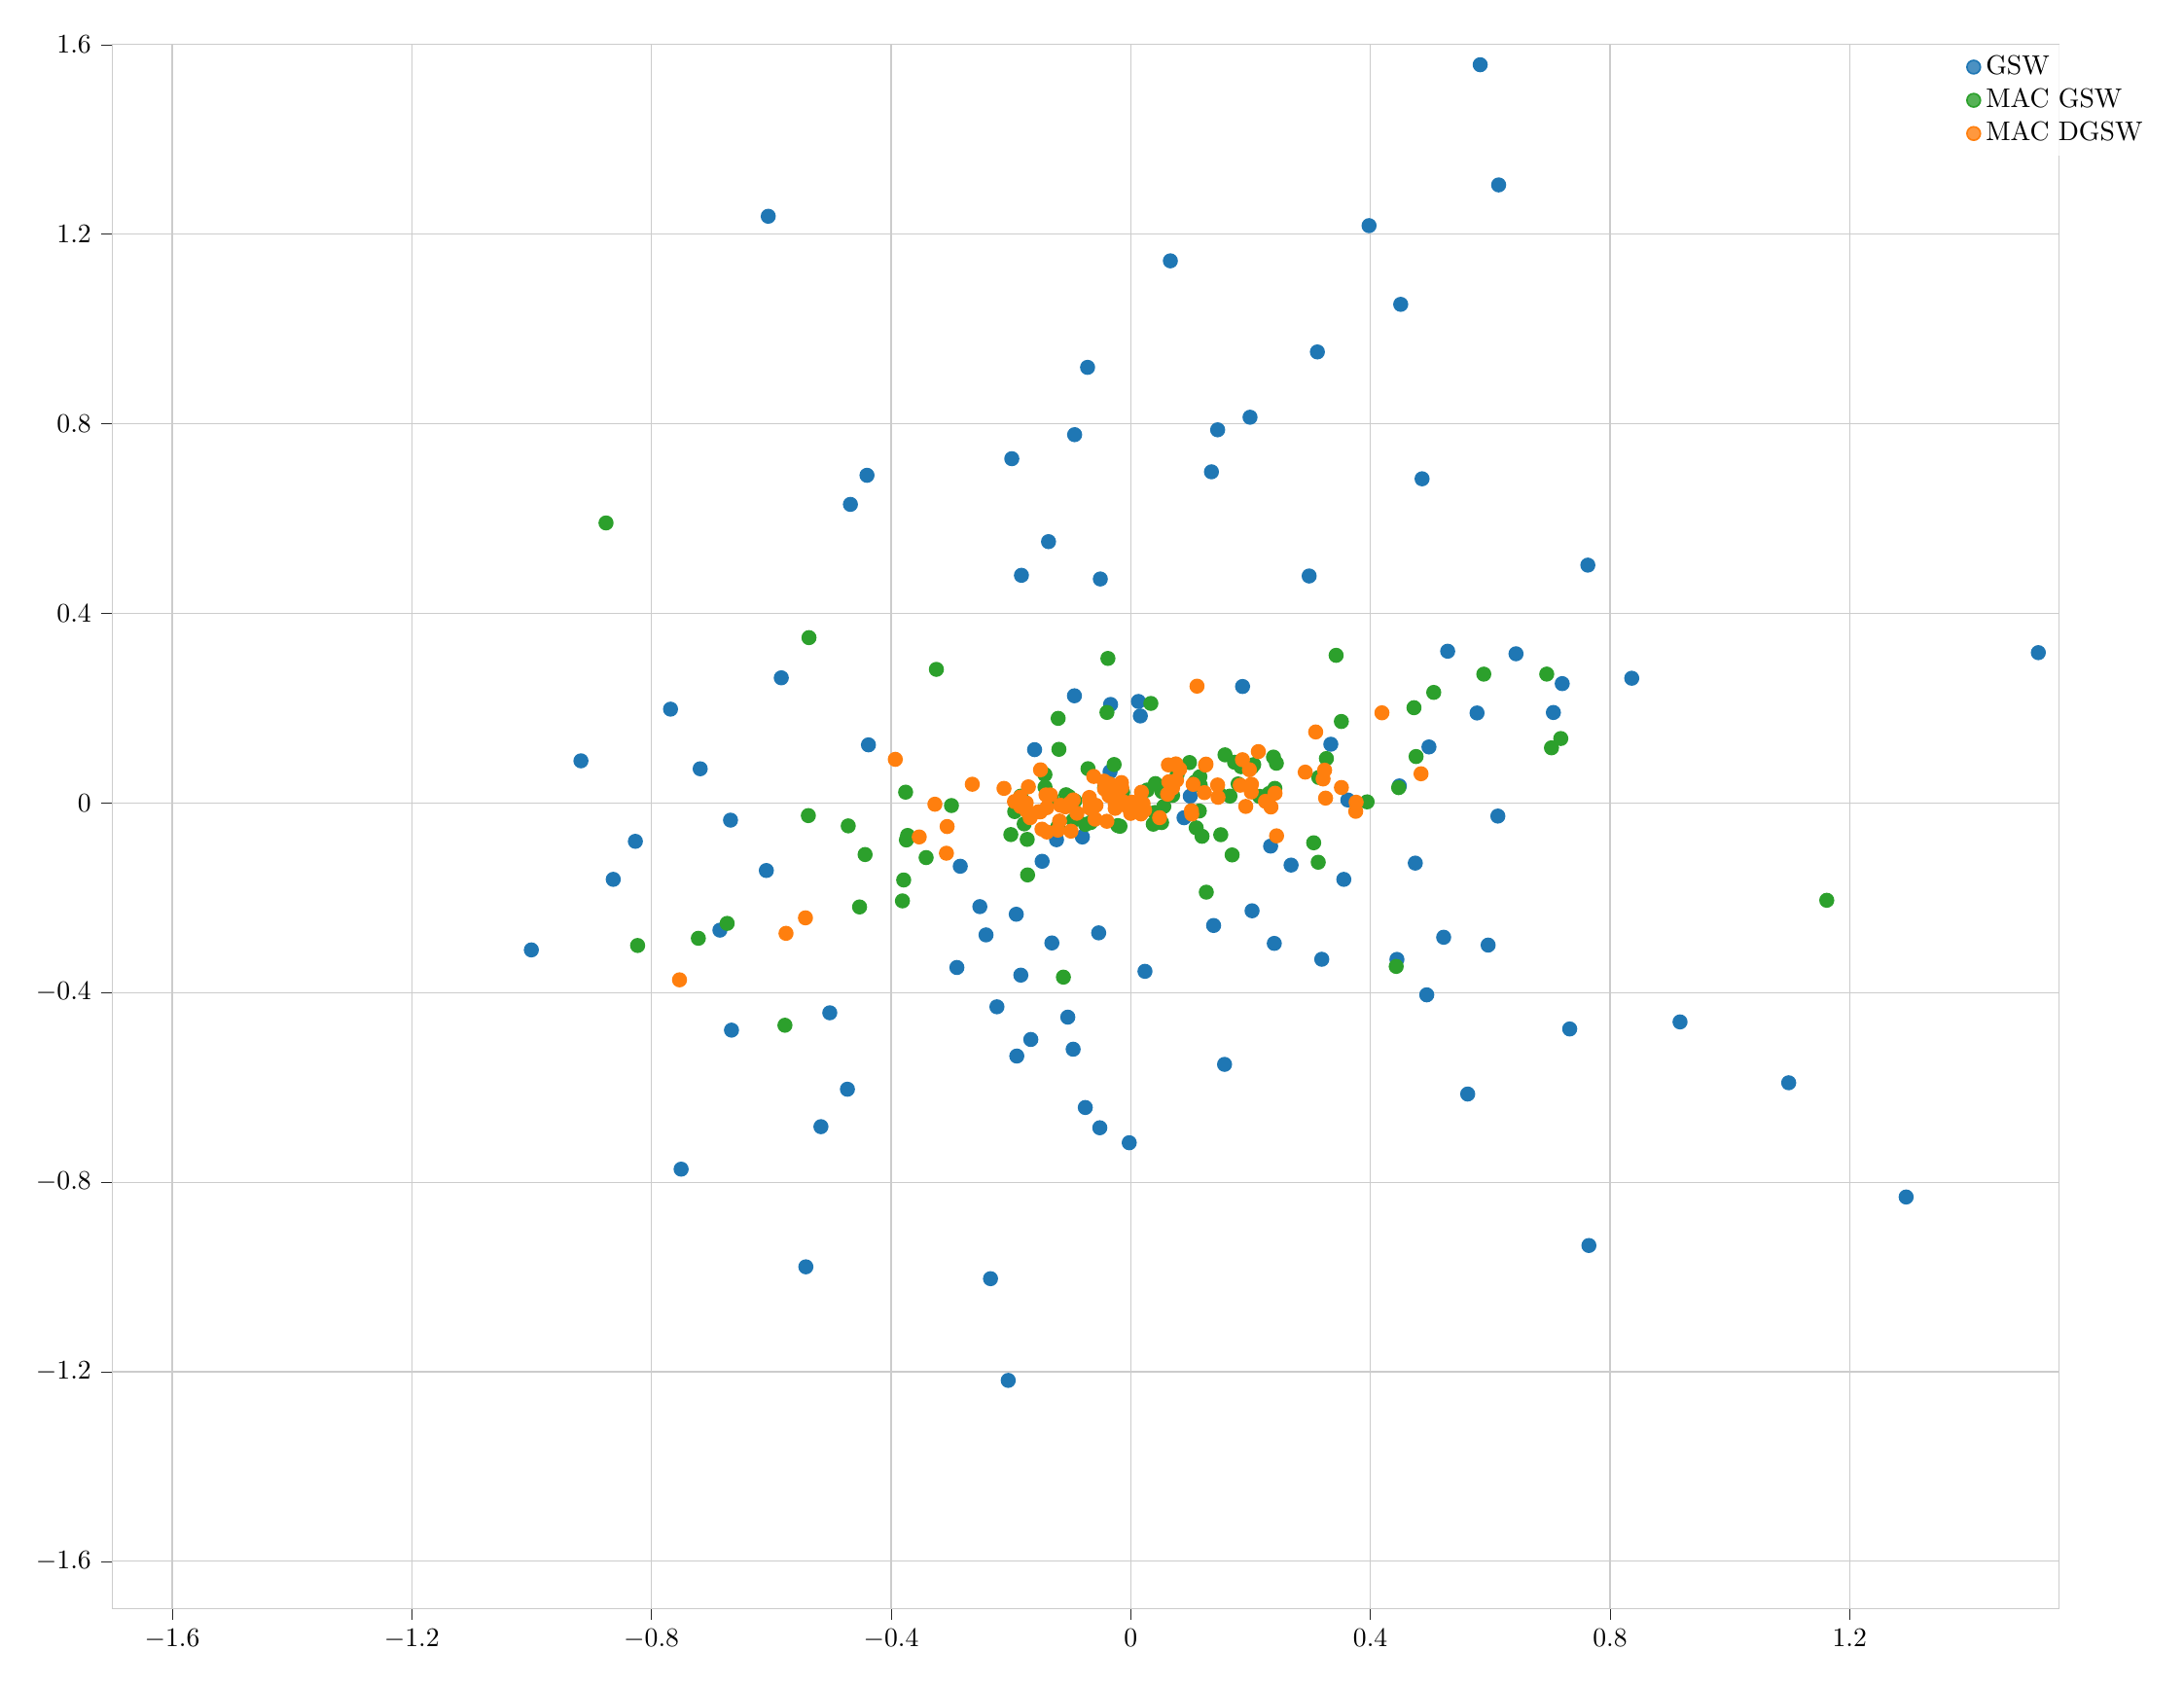
\begin{tikzpicture}

\definecolor{crimson2143940}{RGB}{214,39,40}
\definecolor{darkorange25512714}{RGB}{255,127,14}
\definecolor{darkslategray38}{RGB}{38,38,38}
\definecolor{forestgreen4416044}{RGB}{44,160,44}
\definecolor{lightgray204}{RGB}{204,204,204}
\definecolor{steelblue31119180}{RGB}{31,119,180}

\begin{axis}[
width=27cm,
height=22cm,
axis line style={lightgray204},
legend cell align={left},
legend style={fill opacity=0.8, draw opacity=1, text opacity=1, at={(1.05,1)}, draw=none},
tick align=outside,
tick pos=left,
x grid style={lightgray204},
xmajorgrids,
xmin=-1.7, xmax=1.55,
xtick style={color=darkslategray38},
y grid style={lightgray204},
ymajorgrids,
ymin=-1.7, ymax=1.6,
ytick style={color=darkslategray38},
xtick distance=0.4,
ytick distance=0.4
]
\addplot [semithick, steelblue31119180, mark=*, mark size=2.5, mark options={solid}, only marks]
table {%
-0.234033255900646 -1.00367625019002
-0.502292043921522 -0.442764076039422
0.836281036081821 0.263084517582837
0.138364094176499 -0.258526220858707
0.720248125753671 0.251712751646566
-0.241530179786962 -0.278434880730301
0.0128763064710159 0.214100080883318
-0.204442374925504 -1.21832109870571
-0.608197564356168 -0.14257831092463
-0.0936134180999035 0.776945732312224
-0.00246726984979651 -0.716910161362025
-0.137189984811076 0.551247277714
0.186673795468766 0.2456891065191
0.239637110914271 -0.296353691034541
-0.718623596516722 0.0720362040330895
0.297852963858004 0.478804979559002
-0.750430917872083 -0.772637055145202
0.705507739660454 0.190804869430336
-0.0720022653092329 0.918975982974229
-0.123814909599926 -0.0776276238353677
0.267675758577033 -0.131130422585034
-0.82681530560466 -0.0810171980973629
0.732732709488719 -0.47686808321412
-1.00044502393813 -0.310093229487481
1.29431940394063 -0.831415361862816
0.475008016074183 -0.126943220401025
-0.685714349431893 -0.268399965993668
0.583313456288618 1.55742618164271
0.444369718236827 -0.330112467607311
-0.284503604583435 -0.133606146339581
0.233497309005808 -0.0910962452390574
0.397801468300577 1.2179036546879
-0.050758350904212 0.472484446535623
-0.183434987952764 -0.363305626324016
-0.223302192675715 -0.430129341802673
-0.0534741068054509 -0.274142486626822
0.202541958710536 -0.227564566783066
-0.105038142654043 -0.451936681435429
-0.075848537214351 -0.642583219068994
-0.166753100141519 -0.499067191270763
0.33399504260331 0.123843922697859
-0.0336450301291598 0.207814840092509
0.562472896923732 -0.61414804377299
0.145093422789962 0.787170879612976
0.311567697622262 0.951486970253645
0.91689310603079 -0.462029293363238
-0.517084430567519 -0.683008311536262
0.614135668194764 1.30387815523542
0.529045694787901 0.320050738115971
0.0237974349060753 -0.355277745197299
0.596596302109347 -0.299938385950881
-0.198510437119641 0.726235380064146
-0.0960998131139271 -0.519616751610891
-0.190166247273823 -0.534026535906529
0.764767145434663 -0.933706788175571
0.0889753152224092 -0.0312077873034743
0.36244679028543 0.00624452160930389
0.6128168972278 -0.0277600949820586
-0.191027474026181 -0.234864632153135
0.0160484773037026 0.183466188993843
0.643101908110998 0.314664610624357
-0.440199665544361 0.691239049729156
0.522357308286315 -0.283420746405377
-0.667982451276813 -0.0363005619357031
-0.542228100645402 -0.978698636278002
0.318913269028745 -0.32981670044333
-0.917661964431249 0.0888366355272649
0.0661526864113611 1.14369098033805
0.448420206334977 0.0358587750821122
0.355680921983809 -0.161284019897439
-0.0344789102830596 0.0657710630078346
-0.437768711248302 0.122519762174017
-0.147878149578096 -0.123084827352889
-0.160442437453102 0.112441327899687
-0.467873969950387 0.629851378183047
-0.605004790094052 1.23773238318976
1.09826526258572 -0.590391841218628
0.486323437231879 0.683842148301535
0.49781344085074 0.118138783209857
0.199162579616324 0.813746699815786
0.0994037835743394 0.0143177621005774
0.763008865294524 0.501698765423466
-0.182408913052498 0.480233554589529
-0.472858997530384 -0.60399450758573
-0.290131704232166 -0.347211137555826
0.49412088197899 -0.404874307135683
0.450657852913912 1.05187172477543
-0.0806898339621819 -0.071868882406181
-0.583278838671477 0.263942259852952
0.578072152084348 0.189771221245725
-0.251844989661519 -0.218792848593097
-0.863744368192662 -0.161256459107712
-0.131614768114232 -0.295411293815551
-0.0939281839109833 0.226040429880138
0.156641803715926 -0.551550561227323
-0.666352427418555 -0.479376836175968
-0.768137612744406 0.197861184421593
1.51494426762626 0.317066425699446
0.134735826160048 0.698549161623672
-0.0515880740525029 -0.685313172995431
};
\addlegendentry{GSW}

%\addplot [semithick, darkorange25512714, mark=*, mark size=2, mark options={solid}, only marks]
%table {%
%-0.467038638468901 0.163351498862461
%-0.101919239185745 0.628473700900072
%0.0801924579100065 -0.178704025732937
%0.753187462269824 0.130064491469967
%0.374706860893716 -0.000387992592425224
%-0.665370057589865 0.0977067973338231
%0.652053081628812 0.292598376670511
%0.0148374262245012 0.378243944044846
%0.224735447322395 0.33277893100804
%0.339695432014035 0.220293114276441
%0.694717804129718 -0.484730614404811
%-0.0447768761318819 0.180189466069606
%-0.367025401708594 1.0687999144798
%-0.164054684475613 -0.458662907503445
%0.130221881285737 -0.524035663610767
%0.139814781734605 -0.543560270488167
%-0.962600570869716 -0.405288180125603
%0.973488043120976 -0.856935717130698
%-0.440666815972203 0.280433637963377
%-0.279543693416206 0.647478605973526
%-0.129562555220653 0.0588498091628559
%-0.050620670577852 -0.283010632321553
%0.312804647257637 0.542420767552628
%0.172901039220575 0.308096072147623
%-0.0295902410676738 0.189467024788717
%0.214739519903408 -0.244751086807525
%-0.52024362531045 0.20751662277544
%0.575134510698105 0.192216465590657
%0.150715414211444 -0.711243051143785
%0.765226857889441 0.435857119223086
%-0.227930477381331 1.30418491509201
%-1.34581232354493 0.534977988459928
%0.541398295437146 -0.689140693488258
%0.158009163661221 -0.575798723396934
%-0.110283969633127 -0.737828205205298
%0.294004072225423 0.0636371267252119
%-0.324449474089598 -0.342572150292722
%-0.151939677302189 -0.677225952907154
%0.289978280355074 -1.67142044822281
%0.560658602768102 -0.0849140658534184
%-0.107280888026982 1.15769703648838
%-0.314819239788976 -0.34650834432936
%-1.38391301064195 0.541308226480151
%-0.403737434798016 0.0127302300870335
%-0.217189852665226 -1.26494628164814
%-0.684202923195837 -0.100376911016385
%0.364510233051626 -0.236511476043339
%0.236083118717556 -0.128124242586085
%0.799712056114389 -0.383150421703668
%-0.748713019192892 0.408961673118363
%-0.202722631903016 0.246254463190886
%-0.514198194867251 0.297689359483197
%0.197146403905739 -0.888888552284097
%-0.106590823137342 -0.836970181275125
%0.351658978089219 0.150545401821191
%-0.360664616958125 0.00728441090099902
%-0.772311745710641 -0.748031877030754
%0.803979268759866 -0.532275932049867
%0.404127469582868 0.52052282583965
%0.571727720359632 -0.4122869845535
%-0.49656713035119 0.254312679410066
%-0.473848057608177 -0.462853635482663
%-0.21735193858735 0.160209512945719
%0.348912052619848 -0.0532043387527634
%0.448122238410888 0.0167747642584531
%0.608428829334961 -0.266423999545314
%-0.377289541115829 0.74624134034711
%-0.29943763862136 0.479255261575632
%-1.0799508143577 -0.415839799032266
%-0.0396261025999249 0.231840931307818
%0.262938386809242 0.926279166548501
%-0.422619589658966 0.322946363715624
%-0.233890094862289 0.857701338268492
%-0.260559723624523 -0.343756045118935
%0.0430604414638127 0.754334293069406
%0.0450509234258425 -0.277706956651417
%-0.762037299157703 -1.12434535910064
%-1.70092765813293 -0.260285422727825
%-0.317487208257024 0.0227894113547166
%-0.0958234377251024 0.264701612226168
%-0.323950877294993 -1.18760723318645
%-0.384929040090102 0.309697957903963
%-1.37214395773189 -0.659793972870984
%0.305179407081578 0.588452100742887
%-0.317721638810046 0.228557811586253
%-0.206700043131411 -0.000313817836921138
%-0.532578958505892 0.824388445427596
%-0.132099433765255 -0.83908557519675
%0.790673729882814 0.45270776933461
%0.202017121371984 0.296403517972251
%0.449300888087678 0.053334512732316
%-0.50538117909258 -0.428574039500352
%0.260125371639742 -0.143484256775755
%-0.156476759617417 0.613082101679903
%-1.04544227920129 -0.0632185651588164
%-0.53258455101681 -0.529992899179842
%0.544601773249693 0.241818954253737
%-1.26173673902597 0.205213988866057
%0.192660671855517 0.606290544884742
%0.682584665856881 0.379837987206885
%};
%\addlegendentry{DGSW}
\addplot [semithick, forestgreen4416044, mark=*, mark size=2.5, mark options={solid}, only marks]
table {%
-0.452588602774574 -0.219457519460316
0.476345859537541 0.0978953427767095
-0.172134036025111 -0.151866179644672
-0.0396657886434861 0.190964636126735
0.472817157668971 0.200893147113116
-0.374457774017679 -0.078149422136211
1.16182540485516 -0.20537819098432
-0.0755124028422982 -0.0453587423594553
-0.021250694186526 0.00591169842617756
0.114498859647634 -0.0169505176397957
-0.0276938123583239 0.0810148496112875
0.14969375396652 0.0169376407427895
0.447221674723109 0.0322961476899399
-0.0179316749888104 -0.0492118898425012
-0.200126112195661 -0.0667606289997217
0.15737935214187 0.101437267783666
0.052145845767631 0.0239964360020453
0.126148688291824 -0.188221812062247
0.305412180003018 -0.0840760930397906
-0.721666726034963 -0.285558749136333
-0.172747480854279 -0.0769119456002741
-0.143027073778956 0.0331215668832454
-0.0215992998139061 -0.0477537566915334
0.694392524590123 0.2717972827469
0.20213846865895 0.0756031364328507
0.0552508046433218 -0.00729542986950665
-0.121086237646942 0.178405263015607
0.179342618577572 0.0401050106372966
-0.381015784562271 -0.206682534674106
-0.103020330735049 0.0133818008515392
0.109280628699765 -0.0524947157735565
-0.0436045309481592 0.0319116428663881
0.717826271361302 0.135909663686394
0.702327410990699 0.116280740358789
-0.18357262441467 0.0143560529807855
-0.132321586741959 0.0095982333732853
0.342869252902813 0.311414816003961
0.238284928024251 0.0967131970978064
0.243133392053099 0.0837668590903854
0.184172676340713 0.0765114855097812
0.589323808064775 0.271711416388367
-0.112375218147719 -0.367555419475738
0.077640797486753 0.0609039768626861
-0.673605737892968 -0.254118964628534
-0.119857788044729 0.113067630764945
0.21492665999262 0.0139238402471929
0.240625414196534 0.0307654421395966
0.0403768821095021 -0.0201857966203044
0.173340383895519 0.0858623207290259
0.0980978619403807 0.0852205325145094
0.0101882587167542 -0.00782530215795912
-0.299234588631573 -0.00552398746593336
0.0669749235920836 0.0192430455417744
-0.0670285920129388 -0.041420968277452
-0.341481794137533 -0.11529622529259
-0.378953310834446 -0.162571322653048
0.351603923219323 0.171866440219441
0.115407641915677 0.0552102864977269
0.443123446412395 -0.344928866188997
-0.875785822139023 0.590704877578923
-0.537006404845616 0.348737396631864
0.0411969754590678 0.0407924355875438
0.0698136672868535 0.0160203358858849
-0.375718820001009 0.0227433413507611
-0.823046106197783 -0.300789847174211
-0.143204802744239 0.059737010817174
-0.0899831145902293 -0.0338601753190018
0.165671606473188 0.0144445418355706
-0.0134674860633244 0.0225288219436536
0.20531471583818 0.0808763140579259
0.107472390832947 0.0441193615889207
-0.577153734170454 -0.469032336795373
0.116092580470093 0.037343792022727
-0.471492130020215 -0.0484442264634512
-0.177795342486552 -0.0442462195404794
0.169240160411651 -0.109714681439213
0.0515366746343972 -0.0414838042054453
-0.0712346980302463 0.0722493499102312
0.119034560622277 -0.0703488328239812
-0.0380451427656536 0.304860082254377
0.505770524002574 0.233144975579216
0.0336006398843489 0.209967990026856
-0.372424997164652 -0.0686215382058942
-0.0932944987979305 0.00438616078851911
0.0376116654480543 -0.0448399608999658
-0.0960110854805889 -0.0367298794311169
-0.193660326174418 -0.0182453511125268
-0.443371646852136 -0.108842415006626
-0.538060705063321 -0.0267198262646902
0.326640489319838 0.0936577822292611
-0.12155069079146 -0.0502962347868531
0.23082245011828 0.0198765378934497
0.312980912115538 -0.125105611280891
0.394565201840874 0.00227558535755873
-0.107965869020627 0.0172665394403077
0.150286699401742 -0.0670258963231307
-0.324379012168804 0.281801719790688
0.31386641253924 0.0537285859365982
0.0275597383415886 0.0272938668757595
-0.0113449086065469 0.00309961602242942
};
\addlegendentry{MAC GSW}
\addplot [semithick,darkorange25512714, mark=*, mark size=2.5, mark options={solid}, only marks]
table {%
-0.0259290885910473 -0.0114954142409386
0.101271357186816 -0.0163255681630171
0.321070395965924 0.0505440489372534
-0.140059957970794 -0.0100182357410043
-0.173724007349841 -0.01659947126851
0.0178994088758675 0.0226494928837153
0.323589723140104 0.0690639344764825
-0.121653065697466 -0.0573876017212023
0.145758540288976 0.0118743706290425
-0.542913255689161 -0.242433510301094
-0.044519808936015 0.0460174908431399
-0.264423422334665 0.0394456110189793
-0.0996860933075897 -0.0595836391533731
-0.194042406891768 0.00282331831890043
-0.150840159398639 -0.0188512231886781
-0.00504781942925503 -0.00803396232462489
0.201222555600259 0.0231446372915483
-0.575363458117484 -0.275118126046534
0.0816661332083763 0.0713452730752241
-0.170814674940205 0.0339744541043389
-0.306425737204616 -0.0497798024435666
-5.92512676844681e-05 -0.0220339074893874
0.351673869362231 0.0325244217968411
-0.0686640112706358 0.00434780414224539
-0.753123446011497 -0.373216500117259
0.11068452904831 0.246368423949788
0.30874631939003 0.149719714211031
0.0163944217345366 -0.0171918133635158
0.145029742213559 0.0378682029138547
-0.0617587675667626 0.0558898803027492
-0.0137097546900626 0.0036246259937967
0.484585317000591 0.061541622566999
-0.16779531256401 -0.0311279341558582
0.0482001087126991 -0.0311249338900673
0.419317515267764 0.190112550140946
-0.117238233442065 -0.00487364399628099
0.201547530343832 0.0393796467379078
-0.014863319531324 0.0322127543024764
-0.139901828639746 -0.0612694566959325
0.0231189245805801 -0.0151807269599253
0.125708258622434 0.0818705515724565
-0.0188690361759881 -0.00287549992783936
0.0667146603981974 0.0397880503781795
0.0615173906748752 0.0184856817435434
-0.108933327414126 -0.00824240251889535
0.186514313850463 0.0911723672182451
-0.0154881063237819 0.0429026867853062
-0.174444152662411 9.53316863138709e-05
0.0206273810170188 -0.00139224782225739
0.291282613640035 0.0650094803971125
-0.0258917298780877 -0.00242251785998976
0.0764493482773496 0.0477516389796031
0.0171140202697303 -0.023220488211578
0.240881617500477 0.0204892508265295
-0.150571506393192 0.0698832608038778
-0.0624598421215201 -0.00806022534590595
0.00127917869456717 -0.00259887136416576
-0.0398215158445897 -0.0386487749146161
0.0698264882035515 0.0316239716613911
0.213041256529099 0.108370926590979
0.192018622007245 -0.00735777965802381
0.2249343092522 0.00336225175985977
-0.0897570130146476 -0.0217210910215295
-0.0579589471424498 -0.00510737680028422
-0.154071596242187 -0.0186809814167616
0.123019176489109 0.021721573101557
0.101871203764898 -0.0235054359763387
-0.0362437434355024 0.0154239337308216
-0.0683513562768572 -0.0107507334284637
0.0636355550669276 0.0446815130378973
0.182728075687153 0.0373908375410564
-0.30760575387384 -0.106099048416679
-0.141460295122937 0.0169513047282338
-0.101669373316617 -0.000887061823747592
-0.059534758047632 -0.0342415916737528
-0.0690802470571918 0.011507375166087
-0.32685351536921 -0.00272643822790314
-0.148200441044484 -0.0553101829727871
-0.211529856327678 0.0306700586475537
-0.118787143598226 -0.0380351474304789
0.104195933095623 0.0392436008679081
-0.0317941510545268 0.0145798532192029
0.12478346412891 0.0798784515913161
-0.352992770510152 -0.0717584977079477
-0.034834721109417 0.0398992559646995
0.375539437802883 -0.0177353861727488
0.234084158594843 -0.00856200937626878
-0.184391506391315 0.0122843241158181
0.243452458208886 -0.0694527300099564
0.198123289662619 0.0700542613139712
0.0628562363675892 0.0802458095633186
0.0754791742508432 0.082331090375258
0.376266722862813 0.0014674573418863
-0.134075805746529 0.0169151489769553
-0.0958566581654372 0.00638274823300239
0.325233699994208 0.0101685007957334
0.00189541438991614 0.00157168089287324
-0.39294081003627 0.0919894543494698
-0.183729016246042 -0.00746808728097409
-0.0435006189087979 0.029219668306913
};
\addlegendentry{MAC DGSW}
\end{axis}
\end{tikzpicture}
\caption{Results of experiment 1 from section \ref{exp_plot_max_col}. Plot of vectors of imbalances for the GSW and DGSW with random pivot rule and MAC pivot rule. 100 points for each variant on the graph.}
\label{results_plot_max_col}
\end{figure}
Results are visible in figure \ref{results_plot_max_col}. We can see that as previously, the vector of imbalances from DGSW run are slightly closer to $\textbf{0}$ than those from GSW runs. Additionally, we can see that the MAC pivot rule seems to give us shorter vector of imbalances as well, with MAC DGSW runs being visibly much closer to \textbf{0}. While this effect could be expected as we color the vectors that allow us to pick smaller deltas and thus move less away from \textbf{0}, it is actually very visible here and we will investigate it further in the next experiment.

We also see that the vectors of imbalances from the MAC GSW and especially the MAC DGSW seem visibly skewed along the $x$-axis. While this is not as present if we reproduce this plot with a different input vector sets, we can sometimes see that MAC (D)GSW vectors of imbalances are somewhat more centered along some direction. It would be interesting to see how this direction is related to the input vectors, maybe it is one of the eigenvectors of $\sum_{i\in[n]}\textbf{v}_i\textbf{v}_i^T$ ?

\subsubsection{Experiment 2}\label{exp_norms_max_col}
We run a similar experiment as in section \ref{how_good_at_minimizing_disc}, except the algorithms we use are the classical GSW, the GSW with MAC and the DGSW with MAC.
\subsubsection{Results 2}
\begin{figure}[h!]
\centering
\include{comparative_norms_n=160_repeat=1000_max_dim=32768.0_max_col}
\caption{Results of experiment 2 from section \ref{exp_norms_max_col}. Average norm of 1000 vector of imbalances for $n=5,10,20,40,80,160$ input vectors and in dimensions $d=2$ to $d=2^{15}$, using GSW with both the random pivot rule and the maximal coloring rule, and DGSW with the maximal coloring rule.}
\label{results_plot_max_col_norms}
\end{figure}
We can see the results in Figure \ref{results_plot_max_col_norms}. The GSW and the GSW with MAC are very close, but the DGSW with MAC produces significantly smaller vector of imbalances. While for large dimensions, it doesn't make an enormous difference, for smaller dimensions and larger numbers of vectors, this seems to be divide by more than 2 in comparison to the classical GSW which is a sizable improvement.

\subsubsection{Experiment 3}\label{pivot_colored_coloring_rules}
We reproduce the experiment in section \ref{pivot_colored} but with the MAC and CP rules.

We would expect these methods to have higher pivot-coloring rates as the previous ones, as they're literally choosing elements that are more likely than average to be colored in the next step as their absolute value is closer to 1.
\subsubsection{Results 3}
\begin{table}[h!]
\centering
\caption{Results of our experiments from section \ref{pivot_colored_coloring_rules} on how often is the pivot colored as a function of the pivot choice rule and the input vector set, now with coloring-dependent pivot choice rules. Results are averaged over 100 runs of the GSW each and are proportions between 0 and 1.}
\begin{tabular}{l|ll|ll|ll}
Dimension &\multicolumn{6}{c}{\textbf{2}}\\
Set  & \multicolumn{2}{c}{AEN} & \multicolumn{2}{c}{2G} & \multicolumn{2}{c}{IGN} \\
Rule &MAC&CP&MAC&CP&MAC&CP\\ \hline
GSW  &0.950&0.945&0.590&0.550&0.939&0.900\\
DGSW  &0.965&0.968&0.600&0.566&0.954&0.927\\
\hline
\hline
Dimension &\multicolumn{6}{c}{\textbf{10}}\\
Set  & \multicolumn{2}{c}{AEN} & \multicolumn{2}{c}{2G} & \multicolumn{2}{c}{IGN} \\
Rule &MAC&CP&MAC&CP&MAC&CP\\ \hline
GSW  &0.889&0.840&0.406&0.386&0.758&0.711\\
DGSW  &0.930&0.887&0.444&0.419&0.798&0.769\\
\hline
\hline
Dimension &\multicolumn{6}{c}{\textbf{100}}\\
Set  & \multicolumn{2}{c}{AEN} & \multicolumn{2}{c}{2G} & \multicolumn{2}{c}{IGN} \\
Rule &MAC&CP&MAC&CP&MAC&CP\\ \hline
GSW  &0.834&0.595&0.697&0.532&0.800&0.535\\
DGSW  &0.884&0.623&0.722&0.542&0.825&0.544\\
\end{tabular}
\label{pivot_colored_coloring_rules_results}
\end{table}

Results are visible in table \ref{pivot_colored_coloring_rules_results}. We can see that as predicted, the pivot coloring rates are higher in this experiment than in section \ref{pivot_colored}, but they actually aren't for the 2 groups (2G) vector set using the random pivot. One potential explanation is that the longer vectors are often close to being colored but still harder to color than the small ones despite that, where the random pivot rule actually chooses a smaller vector 50\% of the time. 

For dimension 100 we see that the maximum absolute coloring rule actually yields a much higher pivot coloring rate than its proportional variant, which could be an indication that the fractional coloring become less sure, that is closer to 0 on average, the higher the dimension goes.

We can also notice that the DGSW leads to a higher coloring rate, which makes sense as we choose a pivot that's close to being colored and the DGSW will thus finish coloring it more often that the classical GSW.

\subsection{Can we choose the pivot from the potential update directions or $\textbf{v}^\perp(t)$ ?}\label{pivot_from_v_perp}
Section \ref{fast_computations} lets us compute the update direction and $\textbf{v}^\perp(t)$ for every potential pivot, so we could exploit that and choose among potential update directions, potentially only when we need a new pivot but not necessarily. 

One way to do this is to compute $\textbf{u}_t$ for every potential pivot, compute the resulting two potential moves, choose a $\delta$ for each pivot through the usual martingale setting, then among the chosen $\delta_t\textbf{u}_t$ moves, use the shortest one. We call that pivot rule the random minimum move rule (\textbf{RMM}). Its DGSW equivalent just chooses the shortest move with access to every $\delta$ instead of by having chosen one $\delta$ for each potential pivot preemptively. 

Another way to do so is to choose a pivot with a probability proportional to the inverse of the norm of the expected move, that is, $(2\frac{|\delta_t^+\delta_t^-|}{|\delta_t^+|+|\delta_t^-|}\|\textbf{u}_t\|)^{-1}$. We call this pivot rule the inverse move proportional (\textbf{IMP}).

Both of these rules could be applied to choose a new pivot at each step, regardless of whether or not the current pivot has been colored, or only when a new pivot is needed. Note that it is necessary for the current subgaussianity proofs that the pivot stays the same for as long as it isn't colored, but in this case it could be interesting to change at each time step. When we always choose a new pivot we will add \textbf{ANP} for "always new pivot".

As returning all update directions in a computationally efficient way requires to have $n\leq d$ as that is necessary for the implementation described in section \ref{fast_computations}, we cannot test these rules on similar experiments as those previously done. Thus we test them in section \ref{new_rule_tests}.
%\subsection{Can we force the algorithm to color the pivot vector ?}
%\subsection{What makes it so a vector is colored early outside of its norm and dimensionality ?}
%\subsection{Can we make the algorithm faster with some clever factorization ?}

\section{Finding Structured Subgroups}\label{structured_subgroups}
We will try several experiments aiming to identify structured subgroups hidden in sets of random vectors. The idea is that the GSW should color members of the subgroup early as they should be easier to color as they should balance each other out, and we will look at when the GSW colors which vectors over a large number of runs of the GSW and with various sets of vector and configurations. The ideal case would be if the GSW could help us solve a problem such as the planted clique.

This section is inspired by results such as those in section \ref{smaller_dimensionality}.

One problem that we would like to solve is, given vectors $\textbf{v}_1,\dots,\textbf{v}_{n-k}$ in a ball of radius 1 in some dimension $d$ and $\textbf{v}_{n-k+1},\dots,\textbf{v}_n$ vectors in the same ball such that all their coordinates are positive, we apply a single random rotation to $\textbf{v}_{n-k+1},\dots,\textbf{v}_n$. The random rotation is a random orthonormal matrix obtained via the Gram-Schmidt process from vectors whose coordinates each are uniformly picked in $[0,1]$. We would then like to use the GSW to find $\textbf{v}_{n-k+1},\dots,\textbf{v}_n$, by hoping that they would be colored early in a GSW run on average to balance each other as they are close, similarly to what was done in section \ref{smaller_dimensionality}. We call this problem the \textbf{hidden cluster}.

While one could just compute the norms difference between all pairs of vectors and probably find the cluster, one other way to do so would be to look for the vector that's colored the earliest on average after some number $r$ of GSW runs, and return that vector and the $k-1$ vector that are the closest to it. There are lots of moving parameters here, including $n,k,d$ and the specific GSW variant used. We will investigate when that approach works and when it doesn't. We call this technique the \textbf{early coloring}.

\subsection{How many runs are needed to get a good idea of when a vector is colored on average ?}
In order to investigate that, we created four instances of the hidden cluster with $n=200,k\in\{5,10\},d=200$. We then used our early coloring method five times on each instance with $r=200$ and saw if the results differed over the five runs for each set. As the end results were the same for each time we ran the method independently of which run it was, we concluded that $r=200$ was enough to get a good approximation of the average coloring times for this parametrization at least.

This does not mean that the average coloring time of each vector were very close for each time we ran the technique, but it means that the earliest vector was always the same. While this was for a specific instance of the problem and on a small sample size of different instances, each try took a long time and we weren't able to run more to increase our certainty. There probably exists a smart statistics proof for showing what number is a good number of runs, but that wasn't the focus here.

\subsection{Does the early coloring technique work ?}\label{early_work}
We want to know if the technique makes sense and works, so we created 100 instances of the hidden cluster with $n=200,k\in\{5,10,15\},d=200$, (so 100 for each $k$) and tried our technique with GSW, DGSW, MAC GSW and MAC DGSW, where MAC is defined in section \ref{pivot_colored_coloring_rules}. We then used our early coloring method with $r=200$ and recorded how often the technique successfully identified the hidden cluster. For DGSW with MAC which is actualy fully deterministic given the first pivot assuming random vector input, we made sure to use each of the 200 vectors as starting pivot exactly once.
\subsubsection{Results}
\begin{table}[h!]
\centering
\caption{Results of our experiments from section \ref{early_work} on the early coloring method to solve the hidden cluster problem. The results are the proportion of instances for which the early coloring method worked out of 100 runs for each of the 12 cases.}
\begin{tabular}{l|ll|ll|ll}
$k$  & \multicolumn{2}{c}{5} & \multicolumn{2}{c}{10} & \multicolumn{2}{c}{15}\\
Rule &R&MAC&R&MAC&R&MAC\\ \hline
GSW  &0.23&0.29&0.39&0.46&0.71&0.63\\
DGSW &0.28&0.22&0.5&0.52&0.69&0.7\\
\end{tabular}
\label{early_coloring_method_exp1}
\end{table}
Results are available in table \ref{early_coloring_method_exp1}. We see that the bigger the hidden cluster, the easier it seems to be to find which is expected, among other things because the random chance of finding it is also higher. Nevertheless for each dimension the proportion of runs in which the method works is way higher than the proportion of points that are part of the hidden cluster, so the method seems effective. Using the MAC pivot rule seems to help a little bit, but that is hard to tell for certain and I doubt that the difference is statistically significant with our sample size. On the other hand, the DGSW variant successfully identifies the cluster very slightly more often than the original GSW variant, but this could very well again be because of the small sample size.

\subsection{Can we improve early coloring by choosing the pivot differently ?}\label{new_rule_tests}
We used the two pivots rule described in section \ref{pivot_from_v_perp} and the early coloring technique to see whether they improved the results. For the random minimum move rule, one can notice that as in the first step $\delta^+=-\delta^-$, the first vector picked will always be the same, which let us test very quickly as only a single run was necessary instead of the 200 used previously. Additionally, one can see that there are no difference between the GSW and the DGSW for the early coloring method with this pivot rule, again because the first vector picked is always the same. We do 1000 runs for each case.

For the inverse move proportional rule, we cannot use $r=1$ and the tries take much longer. We are only able to do 50 runs for each case.

We reproduce the experiment from section \ref{early_work}, except with the RMM and IMP pivot rules, and for the former, $r=1$ and 1000 runs. Additionally, we try both with and without changing the pivot at every step.

\subsubsection{Results}
\begin{table}[h!]
\centering
\caption{Results of our experiments from section \ref{new_rule_tests} on the early coloring method to solve the hidden cluster problem using the RMM and IMP pivot choice rule. The results are the proportion of instances for which the early coloring method worked out of 1000 runs for each RMM case and 50 runs for each IMP case.}
\begin{tabular}{l|ll|ll|ll}
$k$  & \multicolumn{2}{c}{5} & \multicolumn{2}{c}{10} & \multicolumn{2}{c}{15}\\
Rule &RMM&IMP&RMM&IMP&RMM&IMP\\ \hline
GSW  &0.279&0.28&0.55&0.54&0.687&0.68\\
GSW ANP&0.26&0.24&0.537&0.54&0.691&0.66
\end{tabular}
\label{early_coloring_method_exp2}
\end{table}
Results are available in table \ref{early_coloring_method_exp2}. Changing the pivot at each iteration doesn't seem to change much, perhaps because in RMM at least, the same pivot could be chosen again as it could still yield the shortest $\textbf{v}^\perp(t)$. The proportions are slightly higher in dimension 10 compared to those observed in section \ref{early_work}, but that doesn't seem to be the case for the other $k$'s who produced similar proportions, so this might just be because of the sample size. Overall this doesn't appear to be an improvement, especially because there are slightly more computations in when using that variant.

 
%\subsection{Can we stop each run earlier ?}
%As we're only interested in which element is colored the earliest on average, we could try stopping early for example between the 50th and 100th time step in order to gain time in the process.

%\subsection{Can we use even less runs for our average ?}

\section{Next Interesting Directions}
It would be interesting to modify the algorithm to be able to divide vectors into $k$ balanced groups rather than only two. While this can be achieved using multiple runs of the algorithm and starting points different from \textbf{0}, it loses some of the important properties of the original algorithm. One idea would be to have the coloring live in $(S_{m-1})^n$ instead of $[-1,1]^n$, where $S_{m-1}$ is  the $(m-1)$-dimensional regular simplex centered in \textbf{0} and $m$ is the number of groups we want to separate our vectors into, but several aspects aren't easy to generalize with this framework.

Another interesting direction would be to explore adding coordinates to the input vectors to convey information, and more generally modifying the vector set to influence the outcome. For example, it is possible to make sure that a pair of vectors are together or not together in a GSW assignment by replacing both vectors in the set by a single vector that is either their sum or difference. There are probably other similar possibilities that could be interesting to explore in that direction.

Yet another interesting area where improvements could be made is using quadratic programming when computing the update direction, similarly to what we do at the end of section \ref{norm_affect_when}. While it might increase the asymptotic running time of the algorithm, doing it only when $\textbf{v}^\perp(t)=\sum_{i=1}^n\textbf{u}_t(i)\textbf{v}_i=\textbf{0}$ means that most of the results about the classical GSW still hold, and this is just a way to force some good properties on our solution by restricting partially the infinity of equally valid solution of the original least-squares problem.

There probably exists a different method to solve the issue described in section \ref{bigger_earlier} that allows us to keep more guarantees and increase the norm of the resulting vectors of imbalances less, potentially by using the tools mentioned in the previous two paragraphs.

There could be a way to adapt what was done in section \ref{structured_subgroups} to problems such as the planted clique, using a smart normalization and a specialized version of the GSW. I did not succeed in consistently solving instances of that problem with a method similar to the one presented for the hidden cluster, but using the GSW to identify structured subsets seems promising. One could also look at coloring step correlations between pairs of element, as one could hope that these measures could be high between two elements of a structured subgroup.

Being able to explicitly compute the distribution of assignments or of vectors of imbalances produced via the GSW without enumerating all potential possibilities could greatly help understand it.

Another interesting experiment could be to actually see how the discrepancy, that is the maximum coordinate in the vector of imbalances rather than the norm of that vector, is actually minimized in some of the experiments we performed. The potential difference in results compared to the experiments already performed would help us understand the behavior of each variant with more details.

It would be interesting to see what the applications of the generalization described in section \ref{different_basis_section} could be, and how the results about subgaussianity can generalize to this variant depending on the basis $\mathcal{B}$.

Finally, applying this algorithm in various field where it could make an impact and seeing how it improves them would be very interesting. For example, using this algorithm to provide balanced training and testing sets when doing machine learning with small data sets could be useful. Additionally, maybe forcing deep learning batches to be balanced or not at different moments of the training procedure could improve training time and help get out of local minimas or do some fine tuning, but given the size of the datasets generally used in deep learning, this might be too computationally expensive to run if done on the whole dataset.
%using the algorithm in machine learning to balance training and testing set, maybe balance batches in deep learning but probably too computationally expensive.
\newpage
%\appendix
%\section{This is an appendix}


\newpage
\nocite{*}
\bibliography{references}
\bibliographystyle{plain}

% Add the References to the table of contents.
\addcontentsline{toc}{section}{References}

\end{document}
